%% LyX 2.3.1 created this file.  For more info, see http://www.lyx.org/.
%% Do not edit unless you really know what you are doing.
\documentclass[oldfontcommands]{mimosis}
%\usepackage[T1]{fontenc}
%\usepackage[latin9]{luainputenc}
% \usepackage[a4paper]{geometry}
% \geometry{verbose,tmargin=3.5cm,bmargin=3.5cm,lmargin=3cm,rmargin=3cm,headheight=1.25cm,headsep=1.25cm,footskip=1.25cm}
\usepackage{multicol}
\usepackage[normalem]{ulem}
\usepackage{color}
\usepackage{mathrsfs}
\usepackage{mathtools}
\usepackage{amsmath}
\usepackage{amssymb}
\usepackage{cancel}
\usepackage{stmaryrd}
\usepackage{graphicx}
\usepackage{wasysym}
\usepackage{xargs}[2008/03/08]
\usepackage{varwidth}

\makeatletter
%%%%%%%%%%%%%%%%%%%%%%%%%%%%%% User specified LaTeX commands.
%\usepackage{my_preamble}
\usepackage{physics}
\usepackage{import}
\usepackage{xifthen}
\usepackage{pdfpages}
\usepackage{transparent}
\usepackage{lmodern,adjustbox}
\usepackage[skins,breakable]{tcolorbox}
\usepackage{pgfplots}
\usepackage{tikz}
\usetikzlibrary{quantikz}
\tcbuselibrary{listings}
\tcbuselibrary{breakable}
\usetikzlibrary{arrows}
\lstset{
basicstyle=\small\ttfamily,
columns=flexible,
breaklines=true
}

\makeatother
%\lstloadlanguages{Latex}

\newtcolorbox{Code}{enhanced,fonttitle=\sffamily\bfseries\large,valign=center
,drop fuzzy shadow,sidebyside, lefthand ratio=0.4,lower separated=false}

\newtcolorbox{Cuadro}[1]{enhanced,fonttitle=\sffamily\bfseries\large,valign=center
,drop fuzzy shadow,width=\linewidth/#1,lefthand ratio=0.4,lower separated=false}

\newcommand{\cobox}[1]{%
    \begin{newtcolorbox}[enhanced,fonttitle=\sffamily\bfseries\large,valign=center
,drop fuzzy shadow,width=#1, lefthand ratio=0.4,lower separated=false]
          \end{newtcolorbox}
                      }
                      

    
    % colback=#1,
    %                   colframe=white,
    %                   skin=beamer,
    %                   drop fuzzy shadow,
    %                   width=5cm,
    %                   left=1ex,right=0.5ex]
    % \large\mbox{}\hfill#2\hfill\mbox{}
    %       \end{newtcolorbox}


\usepackage{babel}
\addto\shorthandsspanish{\spanishdeactivate{~<>.}}



% \documentclass[oldfontcommands]{mimosis}

\makeatletter
\DeclareOldFontCommand{\rm}{\normalfont\rmfamily}{\mathrm}
\DeclareOldFontCommand{\sf}{\normalfont\sffamily}{\mathsf}
\DeclareOldFontCommand{\tt}{\normalfont\ttfamily}{\mathtt}
\DeclareOldFontCommand{\bf}{\normalfont\bfseries}{\mathbf}
\DeclareOldFontCommand{\it}{\normalfont\itshape}{\mathit}
\DeclareOldFontCommand{\sl}{\normalfont\slshape}{\@nomath\sl}
\DeclareOldFontCommand{\sc}{\normalfont\scshape}{\@nomath\sc}
\makeatother

% \makeatother




%%%%%%%%%%%%%%%%%%%%%%%%%%%%%%%%%%%%%%%%%%%%%%%%%%%%%%%%%%%%%%%%%%%%%%%%
% Some of my favourite personal adjustments
%%%%%%%%%%%%%%%%%%%%%%%%%%%%%%%%%%%%%%%%%%%%%%%%%%%%%%%%%%%%%%%%%%%%%%%%
%
% These are the adjustments that I consider necessary for typesetting
% a nice thesis. However, they are *not* included in the template, as
% I do not want to force you to use them.

% This ensures that I am able to typeset bold font in table while still aligning the numbers
% correctly.
\usepackage{etoolbox}

\usepackage[binary-units=true]{siunitx}
\DeclareSIUnit\px{px}

\sisetup{%
  detect-all           = true,
  detect-family        = true,
  detect-mode          = true,
  detect-shape         = true,
  detect-weight        = true,
  detect-inline-weight = math,
}

%%%%%%%%%%%%%%%%%%%%%%%%%%%%%%%%%%%%%%%%%%%%%%%%%%%%%%%%%%%%%%%%%%%%%%%%
% Hyperlinks & bookmarks
%%%%%%%%%%%%%%%%%%%%%%%%%%%%%%%%%%%%%%%%%%%%%%%%%%%%%%%%%%%%%%%%%%%%%%%%

\usepackage[%
  pdfencoding = auto,
  colorlinks = true,
  citecolor  = pan323C,%RoyalBlue,
  linkcolor  = pan323C,%RoyalBlue,
  urlcolor   = pan323C,%RoyalBlue,
  pdftex,hyperfigures,pdfpagelabels,
  ]{hyperref}

\usepackage{bookmark}

%%%%%%%%%%%%%%%%%%%%%%%%%%%%%%%%%%%%%%%%%%%%%%%%%%%%%%%%%%%%%%%%%%%%%%%%
% Bibliography
%%%%%%%%%%%%%%%%%%%%%%%%%%%%%%%%%%%%%%%%%%%%%%%%%%%%%%%%%%%%%%%%%%%%%%%%
%
% I like the bibliography to be extremely plain, showing only a numeric
% identifier and citing everything in simple brackets. The first names,
% if present, will be initialized. DOIs and URLs will be preserved.

\usepackage[%
  autocite     = plain,
  subentry,
  backend      = bibtex, %biber
  doi          = true,
  url          = true,
  giveninits   = true,
  hyperref     = true,
  maxbibnames  = 99,
  maxcitenames = 99,
  sortcites    = true,
  sorting       = none,
  style         = numeric-comp,
  ]{biblatex}
%\addbibresource{Thesis.bib}
\defbibentryset{ZZ.14S}{ZZ.14,ZZ.14b,ZZ.14c}
\defbibentryset{Pr.75S}{Pr.75,Pr.75b}
\defbibentryset{Pr.77S}{Pr.77,Pr.78,Pr.09,Pr.78,Pr.09}
\defbibentryset{FM.07S}{FM.07,FM.07b,FM.07c}
\defbibentryset{MG.69S}{MG.69,MG.69b,MG.69c}
\defbibentryset{HH.11S}{HH.11,HH.11b}
\defbibentryset{LM.15S}{LM.15,LM.15b}
%%%%%%%%%%%%%%%%%%%%%%%%%%%%%%%%%%%%%%%%%%%%%%%%%%%%%%%%%%%%%%%%%%%%%%%%
% Some adjustments to make the bibliography more clean
%%%%%%%%%%%%%%%%%%%%%%%%%%%%%%%%%%%%%%%%%%%%%%%%%%%%%%%%%%%%%%%%%%%%%%%%
%
% The subsequent commands do the following:
%  - Removing the month field from the bibliography
%  - Fixing the Oxford commma
%  - Suppress the "in" for journal articles
%  - Remove the parentheses of the year in an article
%  - Delimit volume and issue of an article by a colon ":" instead of
%    a dot ""
%  - Use commas to separate the location of publishers from their name
%  - Remove the abbreviation for technical reports
%  - Display the label of bibliographic entries without brackets in the
%    bibliography
%  - Ensure that DOIs are followed by a non-breakable space
%  - Use hair spaces between initials of authors
%  - Make the font size of citations smaller
%  - Fixing ordinal numbers (1st, 2nd, 3rd, and so) on by using
%    superscripts

% Remove the month field from the bibliography. It does not serve a good
% purpose, I guess. And often, it cannot be used because the journals
% have some crazy issue policies.
\AtEveryBibitem{\clearfield{month}}
\AtEveryCitekey{\clearfield{month}}

% Fixing the Oxford comma. Not sure whether this is the proper solution.
% More information is available under [1] and [2].
%
% [1] http://tex.stackexchange.com/questions/97712/biblatex-apa-style-is-missing-a-comma-in-the-references-why
% [2] http://tex.stackexchange.com/questions/44048/use-et-al-in-biblatex-custom-style
%
\AtBeginBibliography{%
  \renewcommand*{\finalnamedelim}{%
    \ifthenelse{\value{listcount} > 2}{%
      \addcomma
      \addspace
      \bibstring{and}%
    }{%
      \addspace
      \bibstring{and}%
    }
  }
}

% Suppress "in" for journal articles. This is unnecessary in my opinion
% because the journal title is typeset in italics anyway.
\renewbibmacro{in:}{%
  \ifentrytype{article}
  {%
  }%
  % else
  {%
    \printtext{\bibstring{in}\intitlepunct}%
  }%
}

% Remove the parentheses for the year in an article. This removes a lot
% of undesired parentheses in the bibliography, thereby improving the
% readability. Moreover, it makes the look of the bibliography more
% consistent.
\renewbibmacro*{issue+date}{%
  \setunit{\addcomma\space}
    \iffieldundef{issue}
      {\usebibmacro{date}}
      {\printfield{issue}%
       \setunit*{\addspace}%
       \usebibmacro{date}}%
  \newunit}

% Delimit the volume and the number of an article by a colon instead of
% by a dot, which I consider to be more readable.
\renewbibmacro*{volume+number+eid}{%
  \printfield{volume}%
  \setunit*{\addcolon}%
  \printfield{number}%
  \setunit{\addcomma\space}%
  \printfield{eid}%
}

% Do not use a colon for the publisher location. Instead, connect
% publisher, location, and date via commas.
\renewbibmacro*{publisher+location+date}{%
  \printlist{publisher}%
  \setunit*{\addcomma\space}%
  \printlist{location}%
  \setunit*{\addcomma\space}%
  \usebibmacro{date}%
  \newunit%
}

% Ditto for other entry types.
\renewbibmacro*{organization+location+date}{%
  \printlist{location}%
  \setunit*{\addcomma\space}%
  \printlist{organization}%
  \setunit*{\addcomma\space}%
  \usebibmacro{date}%
  \newunit%
}

% Do not abbreviate "technical report".
\DefineBibliographyStrings{english}{%
  techreport = {technical report},
}

% Display the label of a bibliographic entry in bare style, without any
% brackets. I like this more than the default.
%
% Note that this is *really* the proper and official way of doing this.
\DeclareFieldFormat{labelnumberwidth}{#1\adddot}

% Ensure that DOIs are followed by a non-breakable space.
\DeclareFieldFormat{doi}{%
  \mkbibacro{DOI}\addcolon\addnbspace
    \ifhyperref
      {\href{http://dx.doi.org/#1}{\nolinkurl{#1}}}
      %
      {\nolinkurl{#1}}
}

% Use proper hair spaces between initials as suggested by Bringhurst and
% others.
\renewcommand*\bibinitdelim {\addnbthinspace}
\renewcommand*\bibnamedelima{\addnbthinspace}
\renewcommand*\bibnamedelimb{\addnbthinspace}
\renewcommand*\bibnamedelimi{\addnbthinspace}

% Make the font size of citations smaller. Depending on your selected
% font, you might not need this.
%\renewcommand*{\citesetup}{%
%  \biburlsetup
%  \small
%}

\DeclareLanguageMapping{british}{bibliography-correct-ordinals}
\DeclareLanguageMapping{english}{bibliography-correct-ordinals}

\bibliography{Biblio}


%%%%%%%%%%%%%%%%%%%%%%%%%%%%%%%%%%%%%%%%%%%%%%%%%%%%%%%%%%%%%%%%%%%%%%%%
% Fonts
%%%%%%%%%%%%%%%%%%%%%%%%%%%%%%%%%%%%%%%%%%%%%%%%%%%%%%%%%%%%%%%%%%%%%%%%

\ifxetexorluatex
  \setmainfont{Minion Pro}
\else
  \usepackage[lf]{ebgaramond}
  \usepackage[oldstyle,scale=0.7]{sourcecodepro}
  \singlespacing
\fi

\renewcommand{\th}{\textsuperscript{\textup{th}}\xspace}

\newacronym[description={Principal component analysis}]{PCA}{PCA}{principal component analysis}
\newacronym                                            {SNF}{SNF}{Smith normal form}
\newacronym[description={Topological data analysis}]   {TDA}{TDA}{topological data analysis}

\newglossaryentry{LaTeX}{%
  name        = {\LaTeX},
  description = {A document preparation system},
  sort        = {LaTeX},
}

\newglossaryentry{Real numbers}{%
  name        = {$\real$},
  description = {The set of real numbers},
  sort        = {Real numbers},
}

\makeindex
\makeglossaries
%\renewcommand{\maketitle}{%

%%%%%%%%%%%%%%%%%%%%%%%%%%%%%%%%%%%%%%%%%%%%%%%%%%%%%%%%%%%%%%%%%%%%%%%%
% Incipit
%%%%%%%%%%%%%%%%%%%%%%%%%%%%%%%%%%%%%%%%%%%%%%%%%%%%%%%%%%%%%%%%%%%%%%%%

%\title{\Large{Modelo de Tiempo a Partir de Correlaciones Cuánticas}}
%\subtitle{Tesis Doctoral}
%\author{Alan Boette}
\date{\vspace{-5ex}}

\begin{document}

%\includepdf[pages={1}]{../Figures/caratula.pdf}
%\includepdf[pages={1}]{../Figures/tapa.pdf}


\frontmatter
  \begin{titlepage}
%\vspace*{5cm}
  %\makeatletter
 \begin{center}
        \null\vspace{2pc}
%
        %{\Huge\textit{\textbf{{\color{pan323C}Teoría de la Información Cuántica}}}}
        % \vspace{2pc}
           {\Huge\textbf{\color{pan323C} Computación Cuántica}} 
        %     {\Huge\textit{y en }} 
        %   %  \vspace{2pc}  
        %   {\Huge\textbf{\color{pan323C} Modelos Cuánticos de Tiempo}} \\
           \vspace{2pc}
% %
        \vspace{4pc}
        %{\Large\aldineleft} \\
        \vspace{4pc}
%
%       {\Large\textit{{
%          Unobtrusive Prototyping of \\
%          \vspace{1pc}
%          Activity Streams in Established Spaces}}} \\
%
        \vspace{20pc}
%
        %\@author \\
         {} \\
         \vspace{.5pc}
         {\large  Alan Boette} \\
         \vspace{.5pc}
         {\large  Raúl Rossignoli} \\
    
         \vspace{.5pc}
         %{\large  Paula Pagano} \\
% %
        \vspace{7pc}
%
       
%
       % \vspace{1pc}
%
        \textit{
%        Tesis presentada para optar al grado de Doctor \\
%Facultad de Ciencias Exactas\\
    %    \vspace{1pc}
     %   de la\\
       % \vspace{1pc}
        %Facultad de Ingeniería 
        %Ciencias Exactas \\
        %Departamento de Física \\
        Universidad Nacional de La Plata \\
        }
         {\large 2025} \\
        %\vfill
        %
\includegraphics[width=6cm]{unlpazul.pdf} \\ \medskip
        %\@scm
    \end{center}
     \makeatother
\end{titlepage}

\newpage
\null
\thispagestyle{empty}
\newpage

  \begin{center}
  \textsc{}
\end{center}
%
\noindent
%

Estas notas se basan en los cursos dictados en la {\it Universidad Nacional de La Plata}:

\begin{itemize}
  \item Introducción a a Arquitectura de Computadoras Cuánticas (Facultad de Ingeniería)
  \item Teoría de la Información Cuántica (Facultad de Ciencias Exactas)
\end{itemize}

Actualmente se trata de una versión preliminar por lo que pueden haber errores, partes incompletas o por mejorar. 
Cualquier tipo de sugerencia en este sentido, es bienvenida. \\


 {\it Agradecemos particularmente a Paula Pagano que colaboró con notas del curso, a Mauricio Matera y a Norma Canosa. }

  \tableofcontents

%%%%%%%%%%%%%%%%%%%%%%%%%%%%%%%%

%% Gate matrices and quantum state vectors
\global\long\def\DISTANCIA{\MODULO{\VECTOR{x-x'}}}%

\global\long\def\ROTOR{\VECTOR{\nabla}\times}%
 
\global\long\def\DIVERGENCIA{\VECTOR{\nabla}\cdot}%
\global\long\def\RIRJ{\MODULO{\VECTOR r_{i}-\VECTOR r_{j}}}%
\global\long\def\RRP{\MODULO{\VECTOR r-\VECTOR r'}}%
\global\long\def\POISSON{\LAPLACIAN\Phi=-\frac{\rho}{\epsilon_{0}}}%
\global\long\def\intinf{\int_{-\infty}^{\infty}}%

% \newcommand*{\MacrosDosMilDieciocho}{}


\global\long\def\ACLARACION#1#2{\stackrel{\substack{\mathclap{#1}\\[0.5ex]{\displaystyle \uparrow}\\~ }}{ #2} }%
 
\global\long\def\INDICADORA#1{\mathbf{1}\left\{  #1\right\}  }%

\global\long\def\MODULO#1{\left|\,#1\,\right|}%

\global\long\def\PARENTESIS#1{\left(#1\right)}%

\global\long\def\CORCHETES#1{\left[#1\right]}%

\global\long\def\LLAVES#1{\left\{  #1\right\}  }%

\global\long\def\LKEY#1{\left\{  #1\right.}%

\global\long\def\RKEY#1{\left.#1\right\}  }%

\global\long\def\LCORCHETE#1{\left[#1\right.}%

\global\long\def\RCORCHETE#1{\left.#1\right]}%

\global\long\def\ANGULITOS#1{\left\langle #1\right\rangle }%

\global\long\def\ESPACIOLARGO{\hspace{10mm}}%

\global\long\def\ESPACIOMEDIO{\hspace{5mm}}%

\global\long\def\DEF{\overset{{\scriptstyle \text{def}}}{=}}%

\global\long\def\LLAVEARRIBA#1#2{\overset{{\scriptstyle #2}}{\overbrace{#1}}}%

\global\long\def\LLAVEABAJO#1#2{\underset{{\scriptstyle #2}}{\underbrace{#1}}}%

\global\long\def\REALES{\mathbb{R}}%

\global\long\def\IMAGINARIOS{\mathbb{I}}%

\global\long\def\NATURALES{\mathbb{N}}%

\global\long\def\ENTEROS{\mathbb{Z}}%

\global\long\def\COMPLEJOS{\mathbb{C}}%

\global\long\def\RACIONALES{\mathbb{Q}}%

\global\long\def\DIFERENCIAL{\,d}%

\global\long\def\DIRACDELTA#1{\delta_{D}\PARENTESIS{#1}}%

\newcommand\KRONEDELTA[1][usedefault, addprefix=\global, 1=ij]{\delta_{#1}}%
 

\global\long\def\HEAVYSIDETHETA#1{\Theta_{H}\PARENTESIS{#1}}%

\global\long\def\SINC{\text{sinc }}%

\global\long\def\ATAN{\text{atan}}%

\global\long\def\CURL{\nabla\times}%

\global\long\def\GRADIENT{\nabla}%

\global\long\def\DIVERGENCE{\nabla\cdot}%
 

\global\long\def\LAPLACIAN{\nabla^{2}}%

\global\long\def\REALPART#1{\text{Re}\left(#1\right)}%
\global\long\def\IMAGPART#1{\text{Im}\left(#1\right)}%
\global\long\def\TIENDEA#1{\underset{{\scriptscriptstyle #1}}{\longrightarrow}}%

\global\long\def\EVALUADOEN#1#2#3{\left.#1\right\rfloor _{#2}^{#3}}%

\global\long\def\VECTOR#1{\boldsymbol{#1}}%

\global\long\def\VERSOR#1{\hat{\VECTOR{#1}}}%

\global\long\def\TERA#1{\text{ T}\unit{#1}}%
 

\global\long\def\GIGA#1{\text{ G}\unit{#1}}%

\global\long\def\MEGA#1{\text{ M}\unit{#1}}%

\global\long\def\KILO#1{\text{ k}\unit{#1}}%

\global\long\def\UNIT#1{\,\unit{#1}}%

\global\long\def\CENTI#1{\text{ c}\unit{#1}}%

\global\long\def\MILI#1{\text{ m}\unit{#1}}%

\global\long\def\MICRO#1{\text{ }\mu\unit{#1}}%

\global\long\def\NANO#1{\text{ n}\unit{#1}}%

\global\long\def\PICO#1{\text{ p}\unit{#1}}%

\global\long\def\FEMTO#1{\text{ f}\unit{#1}}%

\global\long\def\PORDIEZALA#1{\times10^{#1}}%

\global\long\def\PROBABILIDAD#1{\mathbb{P}\left(#1\right)}%

\global\long\def\COLOR#1#2{{\color{#2}{\,#1\,}}}%

\global\long\def\RED#1{\textcolor{red}{#1}}%

\global\long\def\BLUE#1{\COLOR{#1}{blue!80!white}}%

\global\long\def\GREEN#1{\textcolor{green!70!black}{#1}}%

\global\long\def\GRAY#1{\COLOR{#1}{black!30}}%

\global\long\def\GRAY#1{\COLOR{#1}{blue!25!white}}%

\global\long\def\GUNDERBRACE#1#2{\GRAY{\LLAVEABAJO{\COLOR{#1}{black}}{#2}}}%

\global\long\def\RUNDERBRACE#1#2{\RED{\LLAVEABAJO{\COLOR{#1}{black}}{#2}}}%

\global\long\def\BUNDERBRACE#1#2{\BLUE{\LLAVEABAJO{\COLOR{#1}{black}}{#2}}}%

\global\long\def\GUPBRACE#1#2{\GRAY{\LLAVEARRIBA{\COLOR{#1}{black}}{#2}}}%

\global\long\def\RUPBRACE#1#2{\RED{\LLAVEARRIBA{\COLOR{#1}{black}}{#2}}}%

\global\long\def\BUPBRACE#1#2{\BLUE{\LLAVEARRIBA{\COLOR{#1}{black}}{#2}}}%
 

\global\long\def\REDCANCEL#1{\RED{\cancel{{\normalcolor #1}}}}%

\global\long\def\BLUECANCEL#1{{\color{blue}\cancel{{\normalcolor #1}}}}%

\global\long\def\BLUECANCELTO#1#2{\BLUE{\cancelto{#2}{{\normalcolor #1}}}}%

%%%%%%%%%%%%%
\global\long\def\KET#1{\left|#1\right\rangle }%

\global\long\def\HAMILTONIANO{\mathscr{H}}%

\newcommand{\VALMEDIO}[1]{\left\langle   #1 \right\rangle}
\newcommand{\EXPECT}[3]{\left\langle#1 |  #3 |#2\right\rangle}
\newcommand{\BRAKETEO}[2]{\left\langle#1 |  #2\right\rangle}
\newcommand{\BRA}[1]{\left\langle #1 \right|}
\newcommand{\PROYECT}[2]{|#1 \rangle\langle   #2|}

\newcommand{\igate}{
  \begin{pmatrix}
    1 & 0 \\
    0 & 1
  \end{pmatrix}
}
\newcommand{\xgate}{
  \begin{pmatrix}
    0 & 1 \\
    1 & 0
  \end{pmatrix}
}
\newcommand{\ygate}{
  \begin{pmatrix}
    0 & -i \\
    i & \phantom{-}0
  \end{pmatrix}
}
\newcommand{\zgate}{
  \begin{pmatrix}
    1 & \phantom{-}0 \\
    0 & -1
  \end{pmatrix}
}
\newcommand{\hgate}{
  \dfrac{1}{\sqrt2}
  \begin{pmatrix}
    1 & \phantom{-}1 \\
    1 & -1
  \end{pmatrix}
}
\newcommand{\sgate}{
  \begin{pmatrix}
    1 & 0 \\
    0 & i
  \end{pmatrix}
}
\newcommand{\phasegate}{
  \begin{pmatrix}
    1 & \phantom{e}0 \\
    0 & e^{i\theta}
  \end{pmatrix}
}
\newcommand{\cnotgate}{
  \begin{pmatrix}
    1 & 0 & 0 & 0 \\
    0 & 1 & 0 & 0 \\
    0 & 0 & 0 & 1 \\
    0 & 0 & 1 & 0 \\
  \end{pmatrix}
}

\newcommand{\qstatezero}{
  \begin{pmatrix}1 \\ 0\end{pmatrix}
}
\newcommand{\qstateone}{
  \begin{pmatrix}0 \\ 1\end{pmatrix}
}


\newtheorem{corollary}{Corolario}
\newtheorem{lemma}{Lema}
\newtheorem{postulate}{Postulado}
\newtheorem{theorem}{Teorema}
% \newcommand{\bra}[1]{\left\langle #1 \right|}
% \newcommand{\ket}[1]{\left|#1\right\rangle}
% \newcommand{\ketbra}[2]{\left|#1\right\rangle \left\langle #2 \right|}
% \newcommand{\braket}[2]{\left\langle#1 |  #2\right\rangle}
% \newcommand{\mel}[3]{\left\langle#1 |  #2 |#3\right\rangle}
%%%%%%%%%%%%%%%%%%%%%%%%%%%%%%%%%%%%%%%

\mainmatter

%%%%%%%%%%%%%%%%%%%%%%%%%%%%%%%%%%%%%%%%%%%%%%%%%%%%%%%%%%%%%%%%%%%%%%%%
\chapter{Introducción}
%%%%%%%%%%%%%%%%%%%%%%%%%%%%%%%%%%%%%%%%%%%%%%%%%%%%%%%%%%%%%%%%%%%%%%%%

%  \begin{minipage}{0.5\textwidth}
%    \begin{small}
 %     ``...'' \par
%\setlength{\parindent}{30ex}
% \begin{flushright}{\it }
% \end{flushright}
%    \end{small}
%    \end{minipage}
%  \vspace{0.5cm}
%\end{center}


%\noindent This package contains a minimal, modern template for writing your
%thesis. While originally meant to be used for a Ph.\,D.\ thesis, you can
%equally well use it for your honour thesis, bachelor thesis, and so
%on---some adjustments may be necessary, though.
\section{Mecánica Cuántica}

La mecánica cuántica es, en resumen, la teoría que describe el funcionamiento de todo el universo, pero que solo se manifiesta en forma directa en ciertos regímenes donde los efectos ``clásicos" son menos relevantes (es decir, a pequeñas longitudes, bajas temperaturas, bajas energías, altas presiones, etc.). Esta teoría presenta varias ideas poco intuitivas pero sin embargo, describe con perfecta precisión numerosos fenómenos que observamos experimentalmente a nivel microscópico. 

En el último tiempo ha habido un crecimiento exponencial en el interés en la teoría de la información 
cuántica y computación cuántica. Numerosas organizaciones gubernamentales y privadas (Google, IBM, Nasa, D-Wave, Microsoft, Russian Quantum Center, Chinese Academy of Sciences, European Flagship Initiative on Quantum Technology, etc.) han estado invirtiendo cifras exorbitantes impulsando la ``carrera'' 
en búsqueda de la computadora cuántica. 

Lo que a principios de los años ochenta 
surgía como la idea ``peculiar'' de utilizar sistemas cuánticos para realizar una tarea
en forma más eficiente que cualquier algoritmo clásico \cite{DEU.85}, 
hoy claramente se ve como un
incipiente cambio de paradigma tecnológico. 
Entre los algoritmos más notables que surgieron inicialmente, se pueden mencionar
el de factorización de Shor \cite{Sh.94}, que logra
una reducción exponencial en el número de pasos requeridos, y el algoritmo cuántico de búsqueda
de Grover \cite{GR.97}, que mostraron el potencial de una computación basada en la mecánica cuántica 
(qubits en lugar de bits \cite{NC.00}). Puede mencionarse también el algoritmo de muestreo bosónico (boson sampling) de Arhikonov \cite{AA.11}, que también logra una reducción exponencial. El protocolo de teleportación cuántica \cite{Be.93} demostró que la 
mecánica cuántica podía también utilizarse para generar nuevas formas de transmisión de información.
Hoy en día son innumerables los desarrollos  que se hacen continuamente, tanto a nivel teórico, experimental 
como incluso a través de la fabricación de dispositivos (como ejemplo de criptografía cuántica: en 2016 China lanzó el satélite QUESS: Quantum Experiments at Space Scale, capaz de recibir y transmitir claves encriptadas).

Entre las características de los sistemas cuánticos que hacen posible estos avances sobresale el entrelazamiento cuántico, término establecido por Edwin Schrödinger en 1935 \cite{Schr.35} 
para referirse a la capacidad de sistemas cuánticos compuestos de exhibir correlaciones entre sus componentes sin análogo clásico.

La determinación exacta del entrelazamiento entre las distintas partes de un sistema compuesto en interacción, es un problema extraordinariamente difícil ya que requiere recursos que crecen exponencialmente con el 
número de componentes.

En estas notas del Curso Teoría de la Información Cuántica, cubriremos los contenidos básicos necesarios para comprender la teoría y los algoritmos de la computación cuántica. 

\section{Notación de Dirac}
Es importante señalar que el formalismo de la mecánica cuántica se basa en el del álgebra lineal, por este motivo es útil introducir algunos conceptos básicos. Tanto en Mecánica Cuántica como especialmente en Computación Cuántica se emplea la notación de ``bra-ket" \; introducida por Dirac.

Es decir, introducimos dos definiciones: el ``bra''  y el ``ket''  que al calcular un producto interno (ver Sección \ref{inner_prod}), forman un  ``bra-ket"  (bracket es corchete en inglés). 

Expresado en forma simple, el ket, escrito como $\ket{\psi}$, donde $\psi$ es una variable arbitraria usada para etiquetar al ket, representa un vector columna de longitud arbitraria. El bra, $\bra{\psi}$ representa su transpuesto conjugado. Para un ejemplo de 2 por 1, el ket $\ket{\psi}$ es tal que
\begin{align}
    \ket{\psi} = 
    \begin{pmatrix}
        \alpha \\
        \beta \\
    \end{pmatrix},\;\;\;
    %\textrm{ y el bra }
    \bra{\psi} = 
    \begin{pmatrix}
        \alpha^\ast & \beta^\ast
    \end{pmatrix}. \nonumber
\end{align}

En general, $\ket{\psi}$ es un vector en un espacio vectorial complejo con producto interno, denominado espacio de Hilbert ${\cal H}$ (o espacio de estados),  mientras que $\bra{\psi}$ es un vector del espacio dual asociado ${\cal H}^*$, tal que $\langle \phi|\psi\rangle$ es el producto interno entre $|\phi\rangle$ y $|\psi\rangle$. En informaci\'on cu\'antica se suelen emplear espacios de  dimensi\'on finita $n$, tal que ${\cal H}=\mathbb{C}^n$, que corresponden a subespacios de un espacio de Hilbert de dimensi\'on infinita. 
\vspace*{-.25cm}

 %For a qubit, we'll define the ground and %excited states with $\ket{0}$ and $\ket{1}$, respectively, as
% \begin{align}
%     \ket{0} = 
%     \begin{pmatrix}
%         1 \\
%         0 \\
%     \end{pmatrix}
%     \textrm{ and }
%     \ket{1} = 
%     \begin{pmatrix}
%         0 \\
%         1 \\
%     \end{pmatrix} \nonumber
% \end{align}
% \noindent which are the real basis vectors of $\mathbb{C}^2$. The full quantum state of one qubit will then be a linear, complex superposition of these two basis vectors which are, by definition, normalized (magnitude one) and orthogonal (inner product zero). An arbitrary qubit state $\ket{\phi} = \alpha\ket{0} + \beta\ket{1}$ for $\alpha,\,\beta \in \mathbb{C}$. The state has corresponding bra $\bra{\phi} = \alpha^\ast\bra{0} + \beta^\ast\bra{1}$. We also impose the restriction $\left|\alpha\right|^2 + \left|\beta\right|^2 = 1$ to normalize the state for reasons to be discussed later in the course.
%\section{Álgebra Lineal en Mecánica Cuántica}
\section{Producto Interno} \label{inner_prod}
Es necesario subrayar ciertos conceptos para aplicar álgebra lineal en mecánica cuántica. En primer lugar el concepto de producto interno usando notación de Dirac. 

En realidad la notación de Dirac permite que el producto interno se calcule de forma sencilla. Por ejemplo, para calcular el producto de $\ket{\psi}$ con sí mismo, simplemente se multiplica por su transpuesto conjugado, que es justamente  $\bra{\psi}$. Por lo que queda: $\braket{\psi}{\psi}$. Para un estado normalizado $\braket{\psi}{\psi}=1$.  %$\sum^\textrm{n}_{i=1}\left|\alpha_i\right|^2=1$, su producto interno será también uno.

Tomando $\ket{\psi}$ perteneciente a $\mathbb{C}^\textrm{n}$, se puede representar $\ket{\psi}$ como una superposición de los elementos de una  base ortonormal $\{|e_i\rangle\,,\;i=1,\ldots,n,\;\langle e_i|e_j\rangle=\delta_{ij}\}$ de  $\mathbb{C}^\textrm{n}$:
\begin{align}
    \ket{\psi} = \sum^\textrm{n}_{i=1}\alpha_i\ket{e_i} \nonumber
\end{align}
\noindent para $\alpha_i \in \mathbb{C}$, 
con $\langle \psi|=\sum_{i=1}^n \alpha_i^*\bra{e_i}$. Para un estado normalizado, 
%Ahora tomando el producto interno consigo mismo, tenemos
\begin{align}
    \braket{\psi}{\psi} &= \sum^\textrm{n}_{i,j=1}\alpha_j^\ast\alpha_i\braket{e_j}{e_i}%\nonumber\\
    %&
    = \sum^\textrm{n}_{i,j=1}\alpha_j^\ast\alpha_i\delta_{ij}%\nonumber\\
    %&
    = \sum^\textrm{n}_{i=1}\alpha_i^\ast\alpha_i%\nonumber\\
    %&
    = \sum^\textrm{n}_{i=1}\left|\alpha_i\right|^2 = 1\nonumber
\end{align}

El producto interno (``overlap'') entre  dos estados diferentes $\ket{\psi}$ y $\ket{\phi}=\sum_{i=1}^n \beta_i |e_i\rangle$ es 
\[\braket{\phi}{\psi} = \sum^n_{i=1}\beta_i^\ast\alpha_i=\langle\psi|\phi\rangle^*\] 
y es un concepto muy importante en mecánica cuántica. 
Para estados normalizados su m\'odulo $|\langle\phi|\psi\rangle|$  está comprendido entre 0 y 1. 
\vspace*{-3cm}

% y se denomina ``overlap" entre los dos estados. 



% \subsection{Operators} \label{operators}
% Next, we consider quantum operators. Simply put, operators act on state vectors and are represented by matrices in the corresponding n-dimensional complex space. Some are defined in infinite dimensional space and must be truncated for finite dimensions. These operators become the classical analog of ``gates" in a quantum algorithm.

% Quantum operators are represented as a variable (often capital) with a hat, eg. \textbf{\^{H}}, \textbf{\^{x}}, or \textbf{\^{a}}, and, in technical terms, are defined as mapping one vector space $V$ to another $W$. For a quantum operator \textbf{\^{A}}, $\textbf{\^{A}}: V \rightarrow W$. They have (but are not limited to) the following properties:

% \begin{enumerate}
%     \item linearity
%         \begin{itemize}
%             \item For quantum operator \textbf{\^{A}} in $V \in \mathbb{C}^\textrm{n}$, $\textbf{\^{A}}\sum^n_i \ket{e_i} = \sum^n_i \textbf{\^{A}}\ket{e_i}$.
%         \end{itemize}
%     \item composites
%         \begin{itemize}
%             \item For quantum operators \textbf{\^{A}}, \textbf{\^{B}} in $V \in \mathbb{C}^\textrm{n}$, $(\textbf{\^{A}\^{B}}) \ket{\psi} = \textbf{\^{A}(\^{B}} \ket{\psi})$
%         \end{itemize}
%     \item commutation
%         \begin{itemize}
%             \item ``Order matters"
%             \item For quantum operators \textbf{\^{A}}, \textbf{\^{B}} in $V \in \mathbb{C}^\textrm{n}$, $\textbf{\^{A}\^{B}}\ket{\psi} \neq \textbf{\^{B}\^{A}} \ket{\psi}$
%             \item In fact, we have the idea of the commutator: The commutator of \textbf{\^{A}} and \textbf{\^{B}} is $[\textbf{\^{A}},\textbf{\^{B}}] = \textbf{\^{A}\^{B}} - \textbf{\^{B}\^{A}}$ and their anti-commutator is $\{\textbf{\^{A}},\textbf{\^{B}}\} = \textbf{\^{A}\^{B}} + \textbf{\^{B}\^{A}}$.
%             \item We say that two operators commute if their commutator is zero.
%         \end{itemize}
% \end{enumerate}

% We have special names for operators with distinct properties. Namely, we call an operator with the property $\hat{\textbf{A}}^\dagger = \hat{\textbf{A}}$ \textbf{hermitian} and an operator with the property $\hat{\textbf{A}}^\dagger\hat{\textbf{A}} = \hat{\textbf{A}}\hat{\textbf{A}}^\dagger = \mathbb{I} \equiv \hat{\textbf{A}}^\dagger = \hat{\textbf{A}}^{-1}$ \textbf{unitary}. Unitary operations are ``reversible" since action on a state with $\hat{\textbf{A}}^\dagger$ will undo the action of \textbf{\^{A}}. Both hermitian and unitary operators are significant for quantum mechanics. We will discuss this in more detail in Section \ref{pos}.

% Some important operators in quantum computing are 

% \noindent identity:
% $\mathbb{I} = 
%     \begin{pmatrix}
%         1 & 0 \\
%         0 & 1 \\
%     \end{pmatrix}\nonumber$
    
% \noindent the Pauli matrices: 
% $\sigma_x = 
%     \begin{pmatrix}
%         0 & 1 \\
%         1 & 0 \\
%     \end{pmatrix}\;
%     \sigma_y = 
%     \begin{pmatrix}
%         0 & -i \\
%         i & 0 \\
%     \end{pmatrix}\;
%     \sigma_z = 
%     \begin{pmatrix}
%         1 & 0 \\
%         0 & -1 \\
%     \end{pmatrix}$
    
% \noindent and the Hadamard:
% $\hat{H} = \frac{1}{\sqrt{2}}
%     \begin{pmatrix}
%         1 & 1 \\
%         1 & -1 \\
%     \end{pmatrix}$.
    
% \noindent We will discuss all of these operators and their function in more detail in future lectures.
    
% \subsection{Tensor Product}
% The tensor product is an important tool for thinking of multiple quantum systems. A single qubit, which, again, is a two-state system, will exist in a complex vector space, called a Hilbert space $\mathcal{H}_A$. If we introduce another qubit into our quantum computer, it will exist in its own Hilbert space $\mathcal{H}_B$. How then, do we talk about these two qubit together?

% Well, with a tensor product. Our full quantum computer system is now the tensor product of the two Hilbert spaces, namely $\mathcal{H}_A \otimes \mathcal{H}_B$. The state of each qubit will exist only in its relevant Hilbert space and an operator in $\mathcal{H}_A$ will only act on a state in $\mathcal{H}_A$ and vice versa. If qubit A is in state $\ket{\psi}$ and qubit B is in state $\ket{\phi}$, then our two-qubit computer is in state $\ket{\psi}_A \otimes \ket{\phi}_B$. Of course, this is generalizable to infinite numbers of qubits, or tensored Hilbert spaces.

% The tensor product carries a few properties:

% \begin{enumerate}
%     \item For $c \in \mathbb{C}$, $c\left(\ket{\psi}_A \otimes \ket{\phi}_B\right) = c\ket{\psi}_A \otimes \ket{\phi}_B = \ket{\psi}_A \otimes c\ket{\phi}_B$
%     \item Distribution: $\left(\ket{\psi_1}_A + \ket{\psi_2}_A\right)\otimes \ket{\phi}_B = \ket{\psi_1}_A \otimes \ket{\phi}_B + + \ket{\psi_2}_A \otimes \ket{\phi}_B$
%     \item Operators act in their own spaces: $\textrm{\^A}_A \otimes \textrm{\^B}_B\left(\ket{\psi}_A \otimes \ket{\phi}_B\right) = \textrm{\^A}_A\ket{\psi}_A \otimes \textrm{\^B}_B\ket{\phi}_B$
% \end{enumerate}

% \noindent We also make a notation simplification:
% \begin{align}
%     \ket{\psi}_A \otimes \ket{\phi}_B = \ket{\psi}\ket{\phi} = \ket{\psi,\,\phi} = \ket{\psi\phi} \nonumber
% \end{align}

% \noindent The tensor product acts as following on vectors and matrices:
% \begin{align}
%     \begin{pmatrix}
%         \alpha\\
%         \beta
%     \end{pmatrix} \otimes
%     \begin{pmatrix}
%         \gamma\\
%         \delta
%     \end{pmatrix} = 
%     \begin{pmatrix}
%         \alpha\gamma\\
%         \alpha\delta\\
%         \beta\gamma\\
%         \beta\delta
%     \end{pmatrix} \nonumber
% \end{align}
% \noindent For an n$\times$m matrix \textbf{A} and p$\times$q matrix \textbf{B}:
% \begin{align}
%     \textbf{A} \otimes \textbf{B} = 
%     \begin{pmatrix}
%         \textrm{A}_{11}\textbf{B} & \textrm{A}_{12}\textbf{B} & \hdots & \textrm{A}_{1\textrm{n}}\textbf{B}\\
%         \textrm{A}_{21}\textbf{B} & \textrm{A}_{22}\textbf{B} & \hdots & \textrm{A}_{2\textrm{n}}\textbf{B}\\
%         \vdots \\
%         \textrm{A}_{\textrm{n}1}\textbf{B} & \textrm{A}_{\textrm{n}2}\textbf{B} & \hdots & \textrm{A}_{\textrm{n}\textrm{n}}\textbf{B}\\
%     \end{pmatrix}\nonumber
% \end{align}

% We call two-qubit states that can be written as the tensor product of two states \textbf{product states} and those that cannot \textbf{entangled states}. For example,
% \begin{align}
%     \ket{\psi} = \frac{1}{2}\left(\ket{00} + \ket{10} - \ket{01} - \ket{11}\right) = \frac{\ket{0} + \ket{1}}{\sqrt{2}} \otimes \frac{\ket{0} - \ket{1}}{\sqrt{2}}
% \end{align}
% is a product state while
% \begin{align}
%     \ket{\Psi^+} = \frac{\ket{00} + \ket{11}}{\sqrt{2}}
% \end{align}
% is not.

\chapter{Postulados de la Mecánica Cuántica\label{ch:postulados}}

\begin{center}
  \begin{minipage}{0.5\textwidth}
    \begin{small}
      ``On ne voit bien qu’avec le coeur. L’essentiel est invisible pour les yeux.'' \par
%\setlength{\parindent}{30ex}
 \begin{flushright}{\it Antoine de Saint-Exupéry}
 \end{flushright}
    \end{small}
\end{minipage}
  \vspace{0.5cm}
\end{center}

\section{Espacio de un Estado Físico}

\begin{postulate}
  A todo sistema físico aislado se le asigna un espacio vectorial complejo dotado de producto interno, es decir, un espacio de Hilbert, el cual se conoce como \emph{espacio del estado} de un sistema. Dicho sistema se describe completamente por un vector unitario que vive en este espacio, llamado \emph{vector estado}.
\end{postulate}

El sistema mecánico cuántico más simple y el de mayor aplicación en este contexto es el \emph{qubit}. Un qubit 
vive un espacio de dos dimensiones.
Supongamos que  $\ket{0}$ y $\ket{1}$ forman un base ortonormal de este espacio.
Luego un vector estado arbitrario se puede escribir como
\begin{equation*}
  \ket{\psi} = a\ket{0} + b\ket{1},
\end{equation*} donde $a$ y $b$ son números complejos. 
La condición de que $\ket{\psi}$ sea unitario, $\braket{\psi}{\psi} = 1$, se la conoce comúnmente como la \emph{condición de normalización} para vectores estado y es imprescindible para que los vectores describan estados físicos. Para el caso del qubit, es entonces equivalente a $|a|^2 + |b|^2 = 1$. 


\paragraph{Superposición.} Decimos que cualquier combinación lineal $\sum_i \alpha_i
\ket{\psi_i}$ es una \emph{superposición} de los estados $\ket{\psi_i}$ con
\emph{amplitud} $\alpha_i$ para el estado $\ket{\psi_i}$.

\section{Evolución}\label{evol}

\begin{postulate}
  La evolución de un sistema cuántico \emph{cerrado} se describe por una 
  \emph{transformación unitaria}. Esto es, el estado $\ket{\psi(t_1)}$ del sistema al tiempo $t_1$ esta relacionado con el estado del sistema $\ket{\psi(t_2)}$ al tiempo 
  $t_2$ a través de un operador unitario $U$ que depende solo de los tiempos $t_1$ y $t_2$, \begin{equation*}
    \ket{\psi(t_2)} = U\ket{\psi(t_1)}.
  \end{equation*}

  De forma equivalente, la evolución de un estado de un sistema cuántico \emph{cerrado} también se describe por \emph{la ecuación de Schr{\"o}dinger}, \begin{equation}
    i\hbar\frac{\mathrm{d}\ket{\psi}}{\mathrm{d}t} = H\ket{\psi}.
    \label{eq:sch-eq}
  \end{equation}
\end{postulate}

En la ecuación de Schr{\"o}dinger, $\hbar=\frac{h}{2\pi}$ se denomina textit{h partida}, donde $h$ es una constante física conocida como la \emph{constante de Planck} cuyo valor se debe determinar experimentalmente. El valor exacto no de relevancia en este contexto por lo que en la práctica es común absorber el factor $\hbar$ dentro de $H$, fijando de forma  efectiva $\hbar = 1$. $H$ es un operador hermítico fijo conocido como el \emph{Hamiltoniano} del sistema cerrado.

Dado que el Hamiltoniano es un operador hermítico tiene una descomposición espectral
\begin{equation}
  H = \sum_E E\ketbra{E}{E}, \label{eq:ham-spec-dec}
\end{equation} con autovalores $E$ y sus correspondientes autovectores normalizados
$\ket{E}$. Los estados $\ket{E}$ convencionalmente se los llama \emph{autoestados de energía}, o a veces \emph{estados estacionarios}, y $E$ es la \emph{energía} del estado $\ket{E}$. A la energía más baja se conoce como el 
\emph{estado fundamental de energía} del sistema, y al  correspondiente autovalor (o autoespacio) de energía se lo conoce como el \emph{estado fundamental}. El motivo por el que en ciertas ocasiones se conoce a los estados $\ket{E}$ como estados estacionarios es porque su único cambio con el tiempo es adquirir un factor numérico global, \begin{equation*}
  \ket{E} \rightarrow \exp(-iEt/\hbar)\ket{E}.
\end{equation*}
La solución a la ecuación de Sch{\"o}dinger's es:
\begin{equation*} \ket{\psi(t_2)} = \exp\left[\frac{-iH(t_2 - t_1)}{\hbar}\right]
    \ket{\psi(t_1)} = U(t_1, t_2)\ket{\psi(t_1)},
\end{equation*} donde definimos \begin{equation}
  U(t_1, t_2) \equiv \exp\left[\frac{-iH(t_2 - t_1)}{\hbar}\right].
  \label{eq:unit-sch-eq}
\end{equation}

La ecuación \ref{eq:unit-sch-eq} refleja la equivalencia entre las dos descripciones de evolución.

\paragraph{\cite{NC.00} Ejercicio 2.54:} Suponer que $A$ y $B$ son operadores hermíticos conmutantes. Probar que $\exp(A)\exp(B) = \exp(A + B)$.

\paragraph{Solución:} Dado que $A$ y $B$ conmutan, se pueden diagonalizar simultáneamente. Escribimos $A = \sum_i a_i\ket{i}\bra{i}$,
$B = \sum_j b_j\ketbra{j}{j}$, notando que $A + B = \sum_i (a_i + b_i)
\ketbra{i}{i}$. Luego, $\exp(A) = \sum_i e^{a_i}\ketbra{i}{i}$, $\exp(B) =
\sum_j e^{b_j}\ketbra{j}{j}$, $\exp(A + B) = \sum_i e^{a_i + b_i}
\ketbra{i}{i}$. Es claro que \begin{align*}
  \exp(A)\exp(B)
  &= \left(\sum_i e^{a_i}\ketbra{i}{i}\right)\left(\sum_j e^{b_j}
    \ketbra{j}{j}\right) \\
  &= \sum_{i, j} e^{a_i}e^{b_j}\ket{i}\delta_{ij}\bra{j} \\
  &= \sum_i e^{a_i}e^{b_i}\ketbra{i}{i} \\
  &= \sum_i e^{a_i + b_i}\ketbra{i}{i} = \exp(A + B),
\end{align*} lo cual prueba el resultado.

% \paragraph{\cite{NC.00} (modified) Exercise 2.55:} Prove that $U(t_1,
% t_2)$ as defined in \eqref{eq:unit-sch-eq} is unitary.

% \paragraph{Solution:} Consider $U(t_1, t_2) = \exp\left[\frac{-iH(t_2 - t_1)}
% {\hbar}\right]$ and $U(t_1, t_2)^\dagger = \exp\left[\frac{iH^\dagger(t_2 -
% t_1)}{\hbar}\right]$. Rewriting $U(t_1, t_2) = \exp(A)$ and $U(t_1,
% t_2)^\dagger = \exp(B)$ where $A$ and $B$ are Hermitian operators, it is clear
% that $A = -B$ and commute. Hence, $\exp(A)\exp(B) = \exp(A + B) = I$.

% \paragraph{\cite{NC.00} Exercise 2.56:} Use the spectral decomposition to
% show that $K \equiv -i\log(U)$ is Hermitian for any unitary $U$, and thus $U =
% \exp(iK)$ for some Hermitian $K$.

% \paragraph{Solution:} Noting that all eigenvalues of $U$ are of modulus 1, one
% could express $U = \sum_i e^{i\theta_i}\ketbra{i}{i}$ with the spectral
% decomposition theorem, leading to $K = -i\log(U) = \sum_i \theta_i\ketbra{i}
% {i}$. Clearly, $K = K^\dagger$, so $K$ is Hermitian.

% \paragraph{} These exercises show that $U(t_1, t_2)$ is unitary. There is
% therefore a one-to-one correspondence between the discrete-time description of
% dynamics using unitary operators, and the continuous time description using
% Hamiltonians.

\section{Medida en Mecánica Cuántica} \label{medidas}

\begin{postulate}
  Las medidas en Mecánica Cuántica se describen por un conjunto de \emph{operadores de medida}: $\{M_m\}$. Estos operadores actúan sobre el estado $\ket{\psi}$ y el índice $m$ hace referencia a la salida del experimento. El estado del sistema después de la medida es 
  
\begin{equation*}
    \frac{M_m\ket{\psi}}{\sqrt{\mel{\psi}{M_m^\dagger M_m}{\psi}}}
\end{equation*}
 y la probabilidad de obtener el resultado $m$ 
está dada por 
\begin{equation*}
    p(m) = \mel{\psi}{M_m^\dagger M_m}{\psi}.
\end{equation*}

Los operadores de medida satisfacen la \emph{ecuación de completitud},
  \begin{equation*}
    \sum_m M_m^\dagger M_m = I.
  \end{equation*}
  La ecuación de completitud expresa el hecho de que la probabilidades suman uno:
  \begin{equation*}
    1 = \sum_mp(m) = \sum_m\mel{\psi}{M_m^\dagger M_m}{\psi}=\bra{\psi}\sum_m M_m^\dagger M_m\ket{\psi}=\bra{\psi}\ket{\psi}  .
  \end{equation*}
A su vez, queda claro que la \textit{condición de normalización} para estados físicos es imprescindible para que las probabilidades esten bien definidas. 
  
\end{postulate}

% \paragraph{\cite{NC.00} Exercise 2.57: (Cascaded measurements are single
% measurements)} Suppose $\{L_l\}$ and $\{M_m\}$ are two sets of measurement
% operators. Show that a measurement defined by the measuerment operators
% $\{L_l\}$ followed by a measurement defined by the measurement operators
% $\{M_m\}$ is physically equivalent to a single measurement defined by
% measurement operators $\{N_{lm}\}$ with the representation $N_{lm} \equiv M_m
% L_l$.

% \paragraph{Solution:} Take $\ket{\psi}$ to be the state of the quantum system
% immediately before both measurements. Then, the state of the system after
% measurement by $L_l$ is \begin{equation*}
%   \ket{\psi'} = \frac{L_l\ket{\psi}}{\sqrt{\mel{\psi}{L_l^\dagger L_l}{\psi}}},
% \end{equation*} and the state of the system after measurement by $M_m$ is
% \begin{equation*}
%   \ket{\psi''} = \frac{M_m\ket{\psi'}}{\sqrt{\mel{\psi'}{M_m^\dagger M_m}
%     {\psi'}}}.
% \end{equation*}
% Noting that $\mel{\psi'}{M_m^\dagger M_m}{\psi'} = \frac{\mel{\psi}{L_l^\dagger
% M_m^\dagger M_m L_l}{\psi}}{\mel{\psi}{L_l^\dagger L_l}{\psi}}$,
% \begin{align*}
%   \ket{\psi''}
%   &= \left(M_m\frac{L_l\ket{\psi}}{\sqrt{\mel{\psi}{L_l^\dagger L_l}{\psi}}}
%   \right)\sqrt{\frac{\mel{\psi}{L_l^\dagger L_l}{\psi}}{\mel{\psi}{
%   L_l^\dagger M_m^\dagger M_m L_l}{\psi}}} \\
%   &= \frac{M_mL_l\ket{\psi}}{\sqrt{\mel{\psi}{L_l^\dagger M_m^\dagger M_m L_l}
%   {\psi}}} \\
%   &= \frac{N_{lm}\ket{\psi}}{\sqrt{\mel{\psi}{N_{lm}^\dagger N_{lm}}{\psi}}}.
% \end{align*}

\section{Distinguiendo estados cuánticos}

Es más simple comprender la distinguibilidad de estados a través de un juego que involucra dos partes, Alice y Bob. Alice elige estados $\ket{\psi_i} (1 \leq i \leq n)$
a partir de un conjunto fijo de estados conocidos para ambos. Ella le da el estado $\ket{\psi_i}$ a Bob, que tiene la tarea de identificar el índice $i$ de el estado que Alice le dió.

Supongamos que los estados $\ket{\psi_i}$ son ortonormales. Luego Bob puede hacer una medida cuántica para distinguir los estados, utilizando el siguiente procedimiento. Define
los operadores de medida $M_i \equiv \ketbra{\psi_i}{\psi_i}$, 
asignando uno a cada índice $i$, y un operador de medida adicional $M_0$ definido como la raíz cuadrad positiva del operador $I - \sum_{i \neq 0}
\ketbra{\psi_i}{\psi_i}$. Estos operadores satisfacen la relación de completitud,
y si el estado $\ket{\psi_i}$ es preparado entonces $p(i) = \mel{\psi_i}{M_i}
{\psi_i} = 1$, por lo que el resultado $i$ ocurre con certeza. 
Luego, es posible distinguir los estados ortonormales $\ket{\psi_i}$.

Por otro lado, si los estados $\ket{\psi_i}$ 
no son ortonormales podemos entonces demostrar que no existe  \emph{medida cuántica capaz de distinguir a los estados}.

\begin{theorem}
  Los estados no ortogonales no se pueden distinguir de manera confiable a través de medidas.

\end{theorem}

\begin{proof}
  Una demostración por el absurdo muestra que no existe una medida que distinga estados no-ortogonales $\ket{\psi_1}$ y $\ket{\psi_2}$. Supongamos que dicha medida sí es posible: 
Si se prepara el estado $\left|\psi_1\right\rangle$
($\left|\psi_2\right\rangle$), luego la probabilidad de medir 
  $j$ tal que $f(j) = 1$ ($f(j)
  = 2$) debe ser 1. Definiendo
$E_i \equiv \sum_{j: f(j) = i}M_j^\dagger M_j$, estas observaciones se pueden escribir como:
\begin{equation*}
\left\langle\psi_1 |  E_1 |\psi_1\right\rangle = 1; \left\langle\psi_2 |  E_2 |\psi_2\right\rangle = 1.
\end{equation*}

Dado que $\sum_iE_i = I$ se ve que
$\sum_i\left\langle\psi_1 |  E_i |\psi_1\right\rangle = 1$, y dado que
$\left\langle\psi_1 |  E_1 |\psi_1\right\rangle = 1$, se debe tener
$\left\langle\psi_1 |  E_2 |\psi_1\right\rangle = 0$, por lo que
$\sqrt{E_2}\left|\psi_1\right\rangle = 0$. Supongamos que descomponemos 
$\left|\psi_2\right\rangle = \alpha\left|\psi_1\right\rangle + \beta\left|\phi\right\rangle$,
donde $\left|\phi\right\rangle$ es ortonormal a
$\left|\psi_1\right\rangle$, $|\alpha|^2 + |\beta|^2 = 1$, y
$|\beta| <
  1$ dado que $\left|\psi_1\right\rangle$ y $\left|\psi_2\right\rangle$
no son ortogonales. Entonces
$\sqrt{E_2}\left|\psi_2\right\rangle = \beta\sqrt{E_2}\left|\phi\right\rangle$,
lo que implica una contradicción, ya que
\begin{equation*}\left\langle\psi_2 |  E_2 |\psi_2\right\rangle = |\beta|^2\left\langle\phi |  E_2 |\phi\right\rangle \leq |\beta|^2
    < 1,
    \end{equation*} 
    donde la última desigualdad surge de la observación de que
 \begin{equation*}
    \mel{\phi}{E_2}{\phi} \leq \sum_i\mel{\phi}{E_i}{\phi} =
    \braket{\phi}{\phi} = 1.
  \end{equation*}
\end{proof}

\section{Medidas Proyectivas}

\paragraph{Medidas Proyectivas.} 

Una medida proyectiva está descripta por un \emph{observable}, $M$, un operador hermítico que actúa sobre el estado del sistema.
Este tiene una descomposición espectral 
\begin{equation*}
M = \sum_m mP_m,
\end{equation*}
donde $P_m$ es un proyector en el autoespacio de $M$ con autovalor $m$.
Las posibles salidas de la medida corresponden a los autovalores,
$m$, de este observable. Midiendo al estado
$\left|\psi\right\rangle$, la probabilidad de obtener el resultado $m$ está
dada por $p(m) = \left\langle\psi |  P_m |\psi\right\rangle.$ Si se obtiene el resultado $m$,
el estado del sistema luego de la medida es
\begin{equation*}
\frac{P_m\left|\psi\right\rangle}{\sqrt{p(m)}}.
\end{equation*}
Las medidas proyectivas son un caso especial en el que los operadores $M_m$ definidos en el Postulado 3, además de satisfacer la relación $\sum_m M_m^\dagger M_m = I$, 
son proyectores ortogonales, es decir, $M_m$ son hermíticos y $M_mM_{m'} = \delta_{m, m'}M_m$.

El promedio de una medida es \begin{align*}
  \langle M \rangle
  &= \sum_m mp(m) \\
  &= \sum_m m\mel{\psi}{P_m}{\psi} \\
  &= \bra{\psi}\left(\sum_m mP_m\right)\ket{\psi} \\
  &= \mel{\psi}{M}{\psi};
\end{align*}
  el valor promedio de un observable $M$ comúnmente se escribe como
  $\langle M \rangle \equiv \left\langle\psi |  M |\psi\right\rangle$. A partir de esta formula para 
  los promedios se obtiene una expresión para la desviación estándar asociada a la observación de $M$,
\begin{equation*}
[\Delta(M)]^2 = \langle (M - \langle M \rangle)^2 \rangle = \langle M^2
  \rangle - \langle M \rangle^2.
  \end{equation*}

% \paragraph{\cite{NC.00} Exercise 2.58:} Suppose we prepare a quantum
% system in an eigenstate $\ket{\psi}$ of some observable $M$, with corresponding
% eigenvalue $m$. What is the average observed value of $M$, and the standard
% deviation?

% \paragraph{Solution:} The average observed value of $M$ is \begin{equation*}
%   \langle M \rangle = \mel{\psi}{M}{\psi} = \mel{\psi}{m}{\psi} =
%   m\braket{\psi}{\psi} = m.
% \end{equation*} Similarly, the average observed value of $M^2$ is
% \begin{equation*}
%   \langle M^2 \rangle = \mel{\psi}{M^2}{\psi} = \mel{\psi}{m^2}{\psi} =
%   m^2\braket{\psi}{\psi} = m^2.
% \end{equation*} It is clear that the standard deviation is $\Delta(M) = \sqrt{
%   \langle M^2 \rangle - \langle M \rangle^2} = \sqrt{m^2 - m^2} = 0$.

% \paragraph{} This formulation of measurement and standard deviations in terms
% of observables gives rise in an elegant way to results such as the
% \emph{Heisenberg uncertainty principle}.

% \begin{proof}[Heisenberg uncertainty principle]
%   Suppose $A$ and $B$ are two Hermitian operators, and $\ket{\psi}$ is a
%   quantum state. Suppose $\mel{\psi}{AB}{\psi} = x + iy$, where $x$ and $y$ are
%   real. Note that $\mel{\psi}{[A, B]}{\psi} = 2iy$ and $\mel{\psi}{\{A, B\}}
%   {\psi} = 2x$. This implies that \begin{equation*}
%     |\mel{\psi}{[A, B]}{\psi}|^2 + |\mel{\psi}{\{A, B\}}{\psi}|^2 =
%     4|\mel{\psi}{AB}{\psi}|^2.
%   \end{equation*} By the Cauchy-Schwarz inequality \begin{equation*}
%     |\mel{\psi}{AB}{\psi}|^2 \leq \mel{\psi}{A^2}{\psi}\mel{\psi}{B^2}{\psi},
%   \end{equation*} which combined with the above equation and dropping a
%   non-negative term gives \begin{equation*}
%     |\mel{\psi}{[A, B]}{\psi}|^2 \leq 4\mel{\psi}{A^2}{\psi}
%     \mel{\psi}{B^2}{\psi}.
%   \end{equation*} Suppose $C$ and $D$ are two observables. Substituting $A = C
%   - \langle C \rangle$ and $B = D - \langle D \rangle$ into the last equation,
%   we obtain Heisenberg's uncertainty principle as it is usually stated:
%   \begin{equation*}
%     \Delta(C)\Delta(D) \geq \frac{|\mel{\psi}{[C, D]}{\psi}|}{2}.
%     \label{eq:hei-unc-prin}
%   \end{equation*}

%   The correct interpretation of the uncertainty principle is that if we prepare
%   a large number of quantum systems in identical states, $\ket{\psi}$, and then
%   perform measurements of $C$ on some of those systems, and of $D$ in others,
%   then the standard deviation $\Delta(C)$ of the $C$ results times the standard
%   deviation $\Delta(D)$ of the $D$ results for $D$ will satisfy the inequality
%   \eqref{eq:hei-unc-prin}.
% \end{proof}

% Rather than giving an observable to describe a projective measurement, often
% people simply list a complete set of orthogonal projectors $P_m$ satisfying the
% relations $\sum_m P_m = I$ and $P_mP_{m'} = \delta_{mm'}P_m$. The corresponding
% observable implicit in this usage is $M = \sum_m mP_m$. Another widely used
% phrase, to `measure in a basis $\ket{m}$', where $\ket{m}$ forms an orthonormal
% basis, simply means th perform the projective measurement with projectors $P_m
% = \ketbra{m}{m}$.

% \paragraph{} Suppose $\vec{v}$ is any real three-dimensional unit vector. Then
% we can define an observable: \begin{equation*}
%   \vec{v} \cdot \vec{\sigma} \equiv v_1\sigma_1 + v_2\sigma_2 + v_3\sigma_3.
% \end{equation*} Measurement of this observable is sometimes referred to as a
% `measurement of spin along the $\vec{v}$ axis', for historical reasons.

% \paragraph{\cite{NC.00} Exercise 2.59:} Suppose we have qubit in the state
% $\ket{0}$, and we measure the observable $X$. What is the average value of $X$?
% What is the standard deviation of $X$?

% \paragraph{Solution:} The average observed value of $X$ is \begin{equation*}
%   \langle X \rangle = \mel{0}{X}{0} = \braket{0}{1} = 0,
% \end{equation*} while the average observed of $X^2$ is \begin{equation*}
%   \langle X^2 \rangle = \mel{0}{X^2}{0} = \braket{1}{1} = 1.
% \end{equation*} Hence, the standard deviation of $X$ is $\Delta(X) = \sqrt{
% \langle X^2 \rangle - \langle X \rangle^2} = \sqrt{1 - 0^2} = 1$.

\subsection{Medidas POVM}

\paragraph{Positive Operator-Valued Measure (POVM).} 
Supongamos que se realiza una medida sobre un sistema cuántico en el estado $\ket{\psi}$ 
descripta por operadores de medida $M_m$.
Luego la probabilidad de obtener el resultado $m$ está dada por
$p(m) = \mel{\psi}{M_m^{\dagger}M_m}{\psi}$. Si definimos
\begin{equation*}
  E_m \equiv M_m^{\dagger}M_m.
\end{equation*} Luego, a partir del Postulado 3 y operaciones de álgebra lineal, se ve que $E_m$ 
es un operador positivo tal que $\sum_mE_m = I$ y $p(m) = \mel{\psi}{E_m}{\psi}$.
Luego el conjunto de operadores $E_m$ permite determinar las
probabilidades de diferentes resultados de medida. 
A los operadores $E_m$ se los conoce como \emph{elementos POVM} asociados
a la medida. Al conjunto completo de los $\{E_m\}$ se los llama \emph{POVM}.

% \paragraph{\cite{NC.00} Exercise 2.62:} Show that any measurement where
% the measurement operators and the POVM elements coincide is a projective
% measurement.

% \paragraph{Solution:} A measurement operator $M_m$ would be defined as a
% POVM element $E_m = M_m^{\dagger}M_m$, which leads to \begin{equation*}
%   \mel{\psi}{E_m}{\psi} = \mel{\psi}{M_m}{\psi} \geq 0
% \end{equation*} for all $\ket{\psi}$. As $M_m$ is a positive operator, it must
% be Hermitian. Therefore, \begin{equation*}
%   E_m = M_m^{\dagger}M_m = M_mM_m = M_m^2 = M_m
% \end{equation*} which, by definition, shows that $M_m$ be a projective
% measurement.

% \paragraph{\cite{NC.00} Exercise 2.63:} Suppose a measurement is described
% by measurement operators $M_m$. Show that there exist unitary operators $U_m$
% such that $M_m = U_m\sqrt{E_m}$, where $E_m$ is the POVM associated to the
% measurement.

% \paragraph{Solution:} Noting that $U_m^{\dagger}U_m = I$, \begin{align*}
%   M_m^{\dagger}M_m
%   &= \sqrt{E_m}U_m^{\dagger}U_m\sqrt{E_m} \\
%   &= \sqrt{E_m}I\sqrt{E_m} \\
%   &= E_m.
% \end{align*}

% \subsection{Phase}

% \paragraph{Phase.} Two amplitudes, $a$ and $b$, \emph{differ by a relative
% phase} if there is a real $\theta$ such that $a = \exp(i\theta)b$.

% [more elaboration needed, the elaboration in my book talks about global phase
% vs relative phase but idk if we'll want to put that in]

% \paragraph{\cite{NC.00} Exercise 2.65:} Express the states $(\ket{0} +
% \ket{1})/\sqrt{2}$ and $(\ket{0} - \ket{1})/\sqrt{2}$ in a basis in which they
% are not the same up to a relative phase shift.

% [idk what the soln for this is supposed to mean either]

\chapter{Fundamentos:}

\section{El Qubit: Quantum Bit}
Un bit cuántico (\emph{qubit}) se describe por un \emph{estado} de dimensión 2. 
Un bit  clásico puede solo tomar valores 0 o 1. De igual forma un qubit puede estar en el estado $\ket{0}$ o $\ket{1}$, que corresponden a los estados de un bit clásico 0 y 1. La diferencia entre un bit y un qubit, es que el qubit puede estar en una \emph{superposición} de $\ket{0}$ y $\ket{1}$ al mismo tiempo.
Este fenómeno se lo puede observar tanto en el espín de un electrón como en la polarización de un fotón. El estado de un qubit se puede describir de la siguiente manera:
\begin{equation}
  \ket{\psi} = \alpha\ket{0} + \beta\ket{1},
\end{equation}
donde $\alpha$ y $\beta$ son números complejos. Aquí $\alpha$ y $\beta$ son las \emph{amplitudes de probabilidad}, y $\ket{0}$, $\ket{1}$ se denominan estados de la \emph{base estándar computacional}.

Las amplitudes de un qubit no se pueden determinar directamente, es necesario medirlo. Si lo medimos, podemos obtener $\ket{0}$ con probabilidad $|\alpha|^2$, o $\ket{1}$ con probabilidad $|\beta|^2$. 
La suma de los valores absolutos al cuadrado de las amplitudes siempre suman 1 por el hecho de tratarse de probabilidades. Esto está garantizado por la condición de normalización de los estados físicos, anteriormente mencionada ($|\alpha|^2 + |\beta|^2 = 1$).

Por ejemplo midiendo al qubit en el estado
\begin{equation}
  \dfrac{1}{\sqrt2}\ket{0}+\dfrac{1}{\sqrt2}\ket{1}
\end{equation}
se obtiene $\ket{0}$ la mitad de las veces y $\ket{1}$ la otra mitad ($|1/\sqrt2|^2 = 0.5$). Este estado se lo denota $\ket{+}$.

\subsection{La Esfera de Bloch}
La esfera de Bloch es la representación geométrica del estado de un qubit. Es un sistema de coordenadas esféricas en el cual un estado cuántico se lo puede describir como
\begin{equation}
  \ket{\psi} = e^{i\delta} \left(\cos\dfrac{\theta}{2}\ket{0} + e^{i\phi}\sin\dfrac{\theta}{2}\ket{1}\right),
\end{equation}
donde $\delta, \theta$ y $\phi$ son números reales. 
El factor $e^{i\delta}$ es una fase global del estado. 
Este factor no influye en las probabilidades de medida, ya que $\left|e^{i\delta}\right| = 1$, por lo que es usual omitirlo, permitiéndonos escribir
\begin{equation}
  \ket{\psi} = \cos\dfrac{\theta}{2}\ket{0} + e^{i\phi}\sin\dfrac{\theta}{2}\ket{1}.
\end{equation}
Los números $\theta$ y $\phi$ definen un punto en la esfera tridimensional (Figure~\ref{fig:bloch}). 
La esfera de Bloch es muy útil para visualizar operaciones de un qubit. Sin embargo, existen limitaciones para generalizar la esfera de Bloch a muchos qubits.
\begin{figure}[ht]
  \centering
  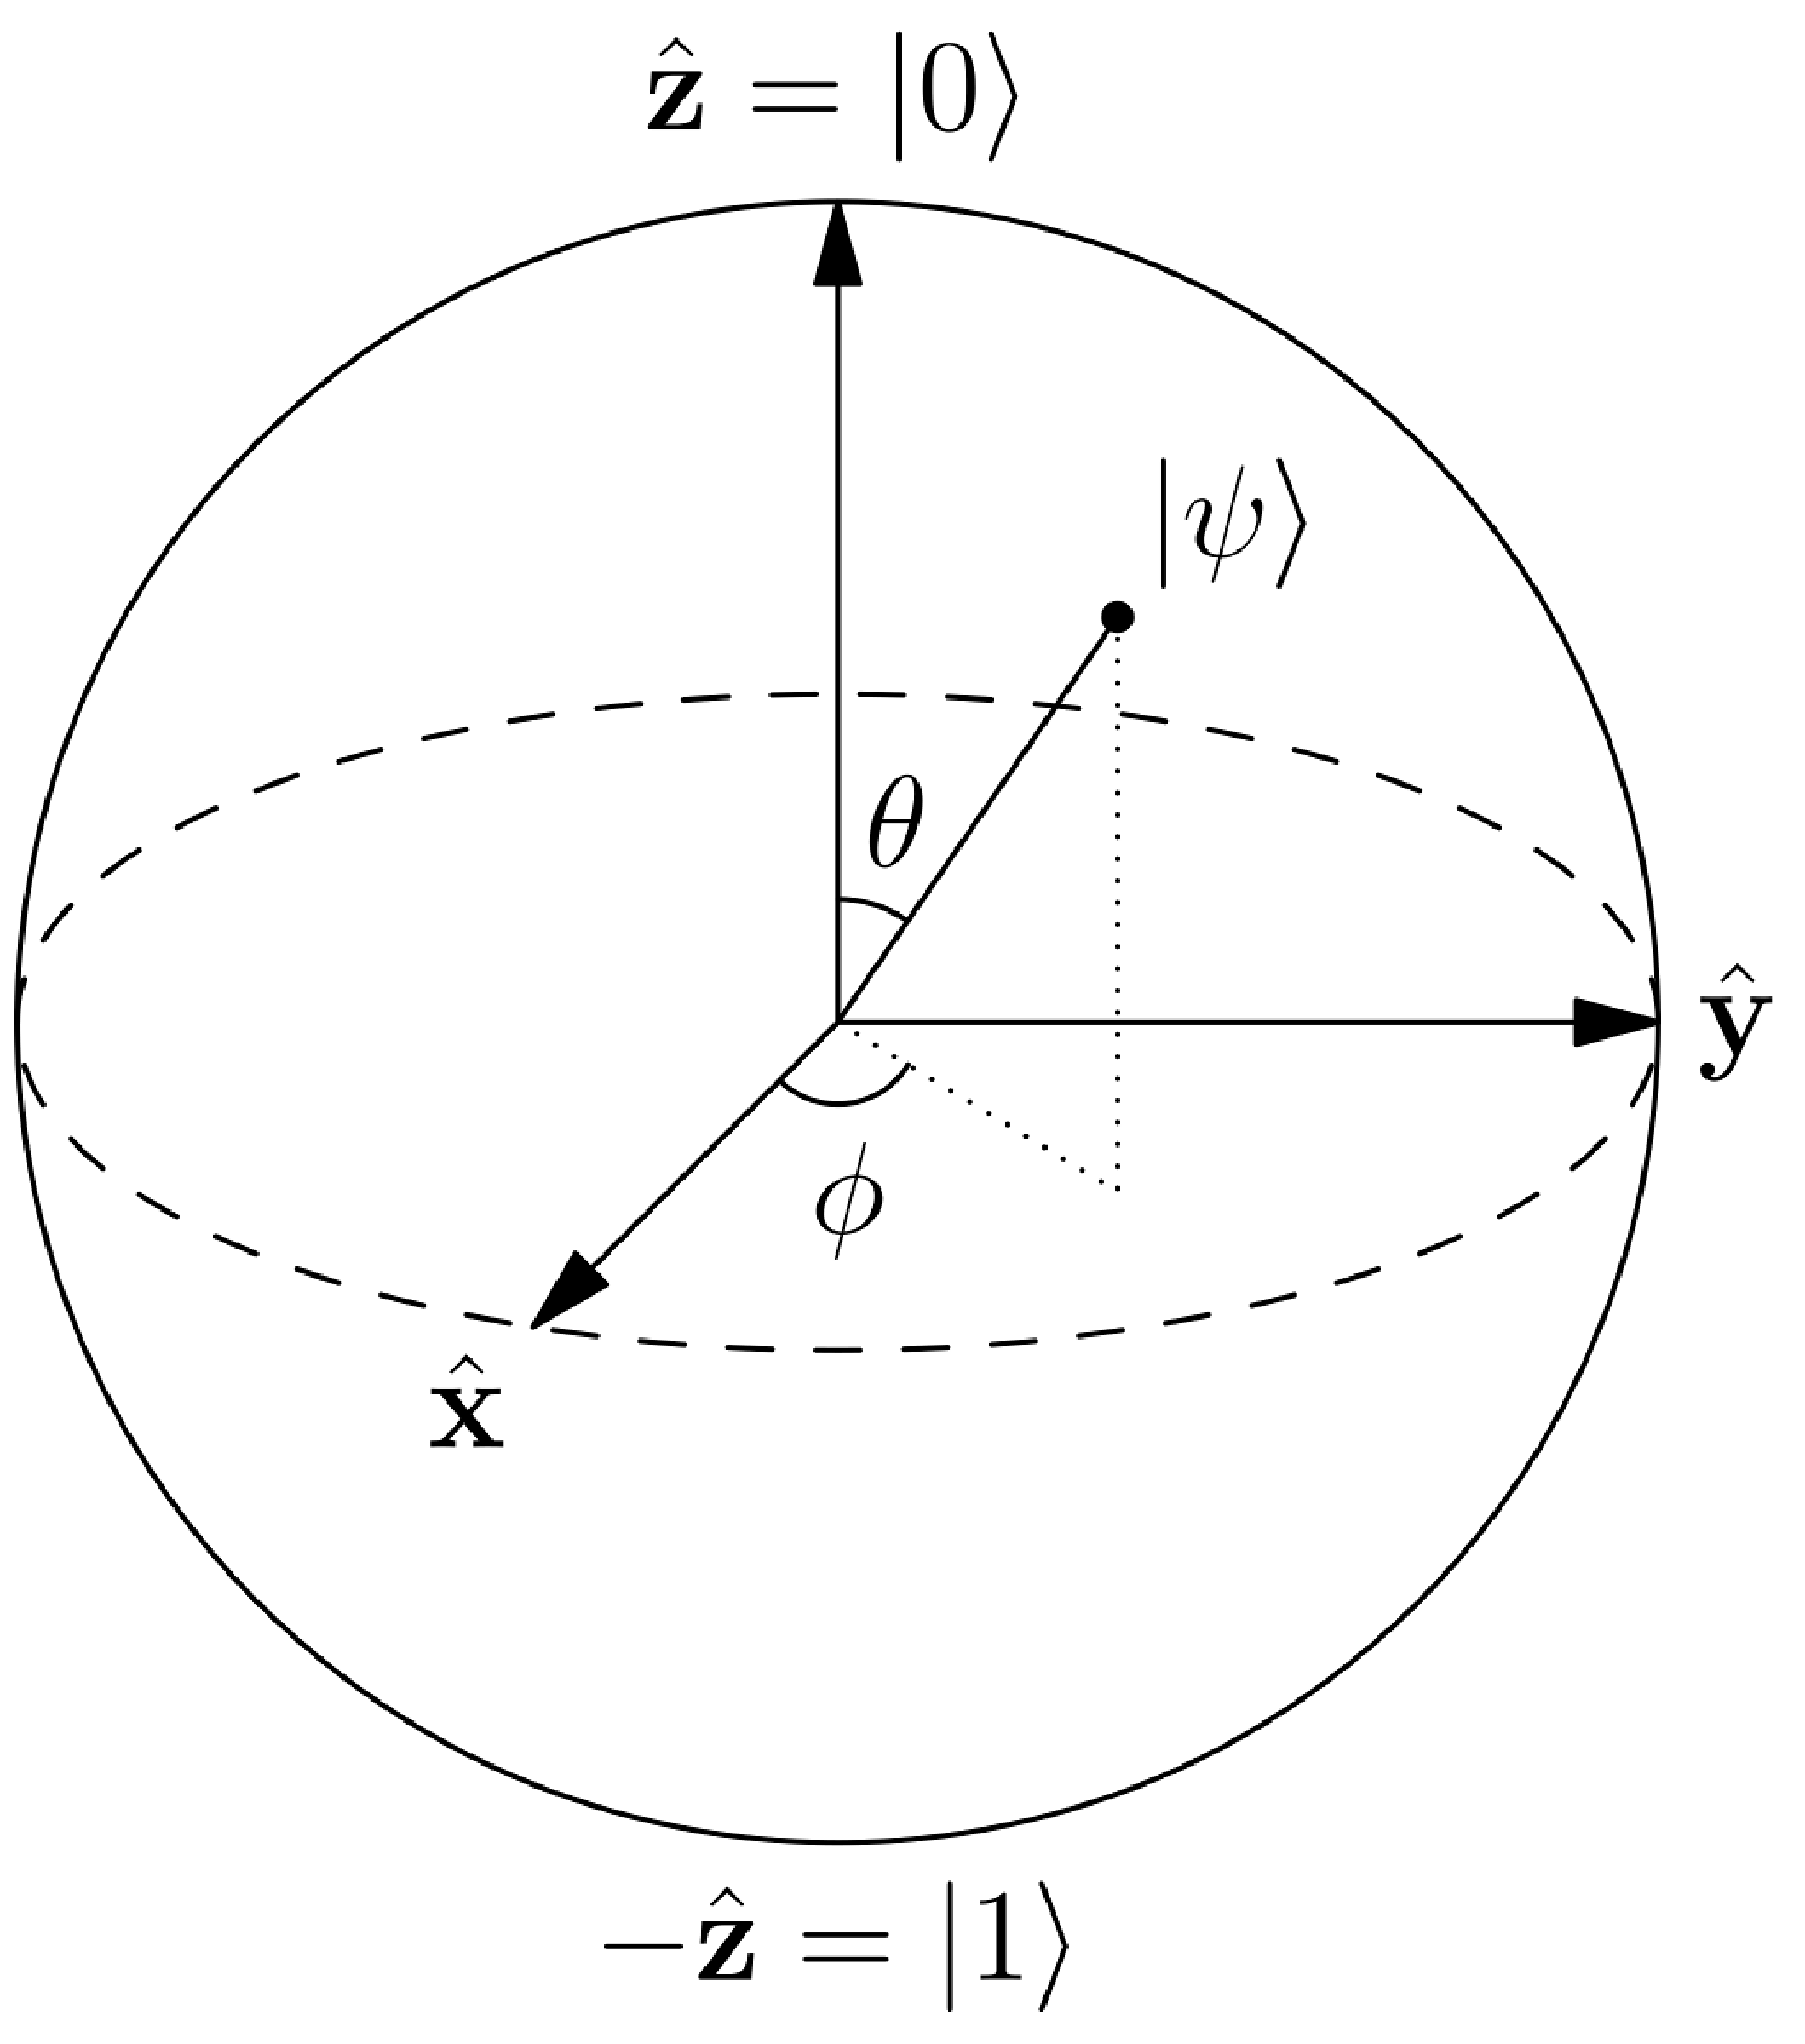
\includegraphics[scale=0.175]{Figures/bloch-sphere.eps}
  \vspace{2mm}
  \caption{Representación de un qubit en la esfera de Bloch.}
  \label{fig:bloch}
\end{figure}

\subsection{Compuertas de un qubit: Single-Qubit Gates}
Las compuertas de un qubit se pueden ver como rotaciones en la esfera de Bloch. Estas compuertas son \emph{unitarias}, es decir $U^\dagger U = UU^\dagger = I$, donde $U^\dagger$ es
la transpuesta conjugada de $U$ y $I$ la identidad. Por lo que cualquier unitaria de $2^n \times 2^n$ es una compuerta válida que actúa en $n$ qubits. Comúnmente $\ket{\psi'} = U\ket{\psi}$ se representan a través un circuito:
\begin{center}
\begin{quantikz}
\lstick{$\ket{\psi}$} & \gate{U} & \qw & \rstick{$\ket{\psi'}$}\qw
\end{quantikz}
\end{center}
% \[
%   \Large
%   \Qcircuit @C=1em @R=0em {
%     & \lstick{\ket{\psi}} & \gate{U} & \qw & \ket{\psi'}
%   }
% \]
A continuación se describen y visualizan algunas compuertas de un qubit usuales.

\subsection{Compuertas de Pauli}\label{pauli_gates}
 Las compuertas de un qubit más simples son las matrices de \emph{Pauli:} $I$, $X$, $Y$ y $Z$. Donde $I$ es la identidad y las compuertas $X$, $Y$ y $Z$ rotan $\pi$ radianes alrededor de los ejes X, Y o Z, respectivamente. 
 
\begin{figure}[ht]
  \centering
  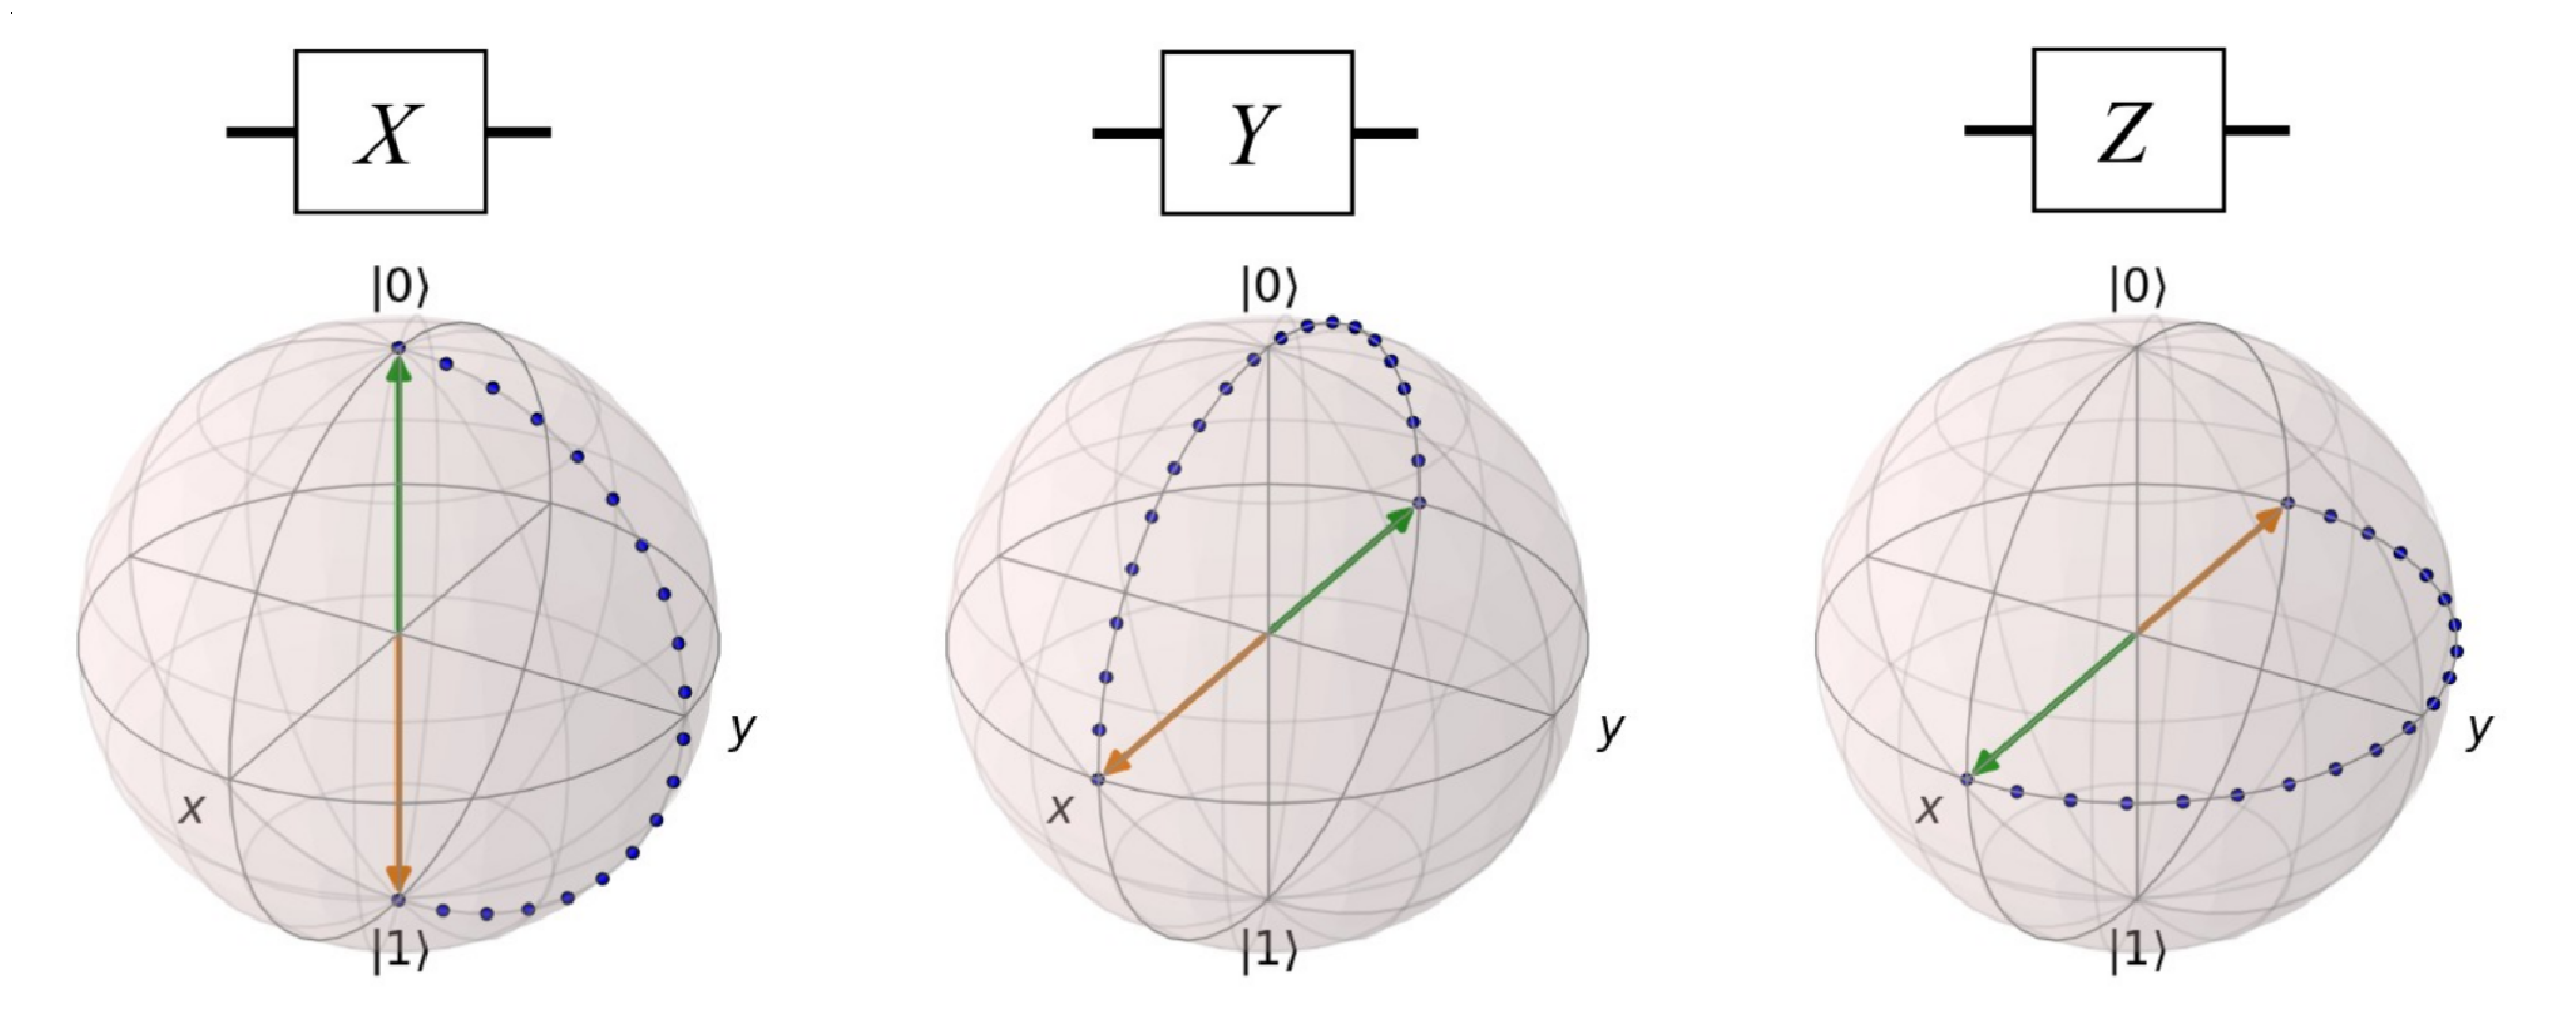
\includegraphics[scale=0.175]{pauli-gates.eps}
  \vspace{2mm}
  \caption{Compuertas $X$, $Y$ y $Z$ visualizadas en la esfera de Bloch. El vector inicial está en verde y el naranja es el de la posición final.}
\end{figure}

\subsection{Compuerta Hadamard}
La compuerta \emph{Hadamard} ($H$) (Figura \ref{fig:hadamard_bloch}) mapea los estados de la base estándar $\ket{0}$ y $\ket{1}$ a estados de superposición con pesos iguales:
\begin{align}
  H\ket{0} &= \dfrac{1}{\sqrt2}(\ket{0} + \ket{1}) = \ket{+} \\
  H\ket{1} &= \dfrac{1}{\sqrt2}(\ket{0} - \ket{1}) = \ket{-}.
\end{align}
Es la combinación de dos rotaciones  de $\pi$ alrededor del eje Z seguidas de una $\pi/2$ alrededor del eje. También se la puede ver como una rotación de $\pi$ alrededor del eje $n=(1,0,1)/\sqrt{2}$.

\begin{figure}[ht]
  \centering
  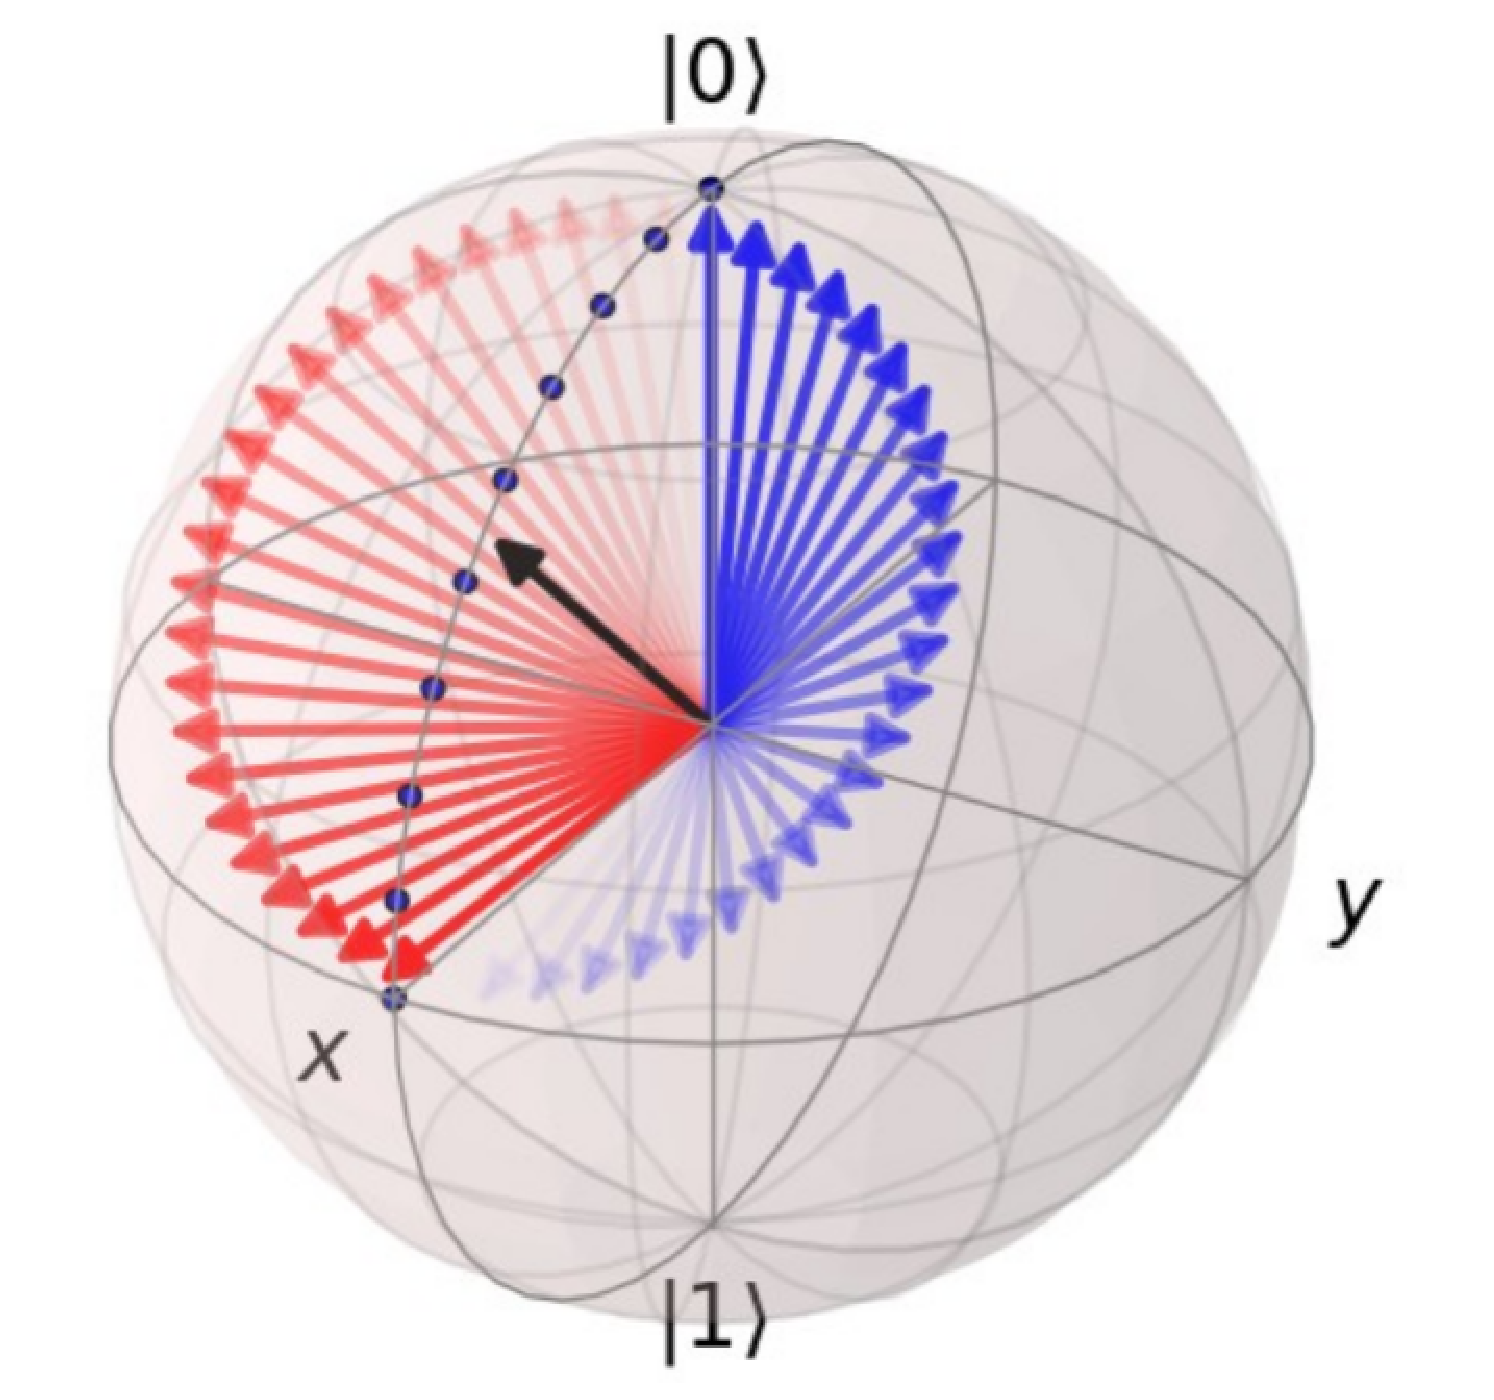
\includegraphics[scale=0.17]{hadamard-gate.eps}
  \vspace{1mm}
  \caption{Visualización de la compuerta Hadamard en la esfera de Bloch.}
  \label{fig:hadamard_bloch}
\end{figure}

\subsection{Compuerta Fase}
Compuertas de que rotan alrededor del eje Z se llaman \emph{Compuertas Fase}. Rotan la fase del estado $\ket{1}$
un ángulo $\theta$ dejando igual al estado $\ket{0}$:
\begin{equation}
  \begin{aligned}
    R_z(\theta) \ket{0} &= \ket{0} \\
    R_z(\theta) \ket{1} &= e^{i\theta}\ket{1}.
  \end{aligned}
\end{equation}
La probabilidad de medir $\ket{0}$ o $\ket{1}$ no cambia al aplicar la compuerta fase, como su nombre lo indica solo cambia la fase del estado cuántico. Una compuerta fase común es la compuerta $S$, donde $\theta = \pi/2$ (Figure \ref{fig:s_bloch}). La compuerta Pauli Z 
se puede pensar como una compuerta fase con $\theta = \pi$ (dado que $e^{i\pi} = -1$). Por lo que se puede pensar a la compuerta $S$ como la mitad de la compuerta $Z$.
Otra compuerta fase conocida es la compuerta $T$,
donde $\theta = \pi/4$ (la mitad de una compuerta $S$).

\begin{figure}[ht]
  \centering
  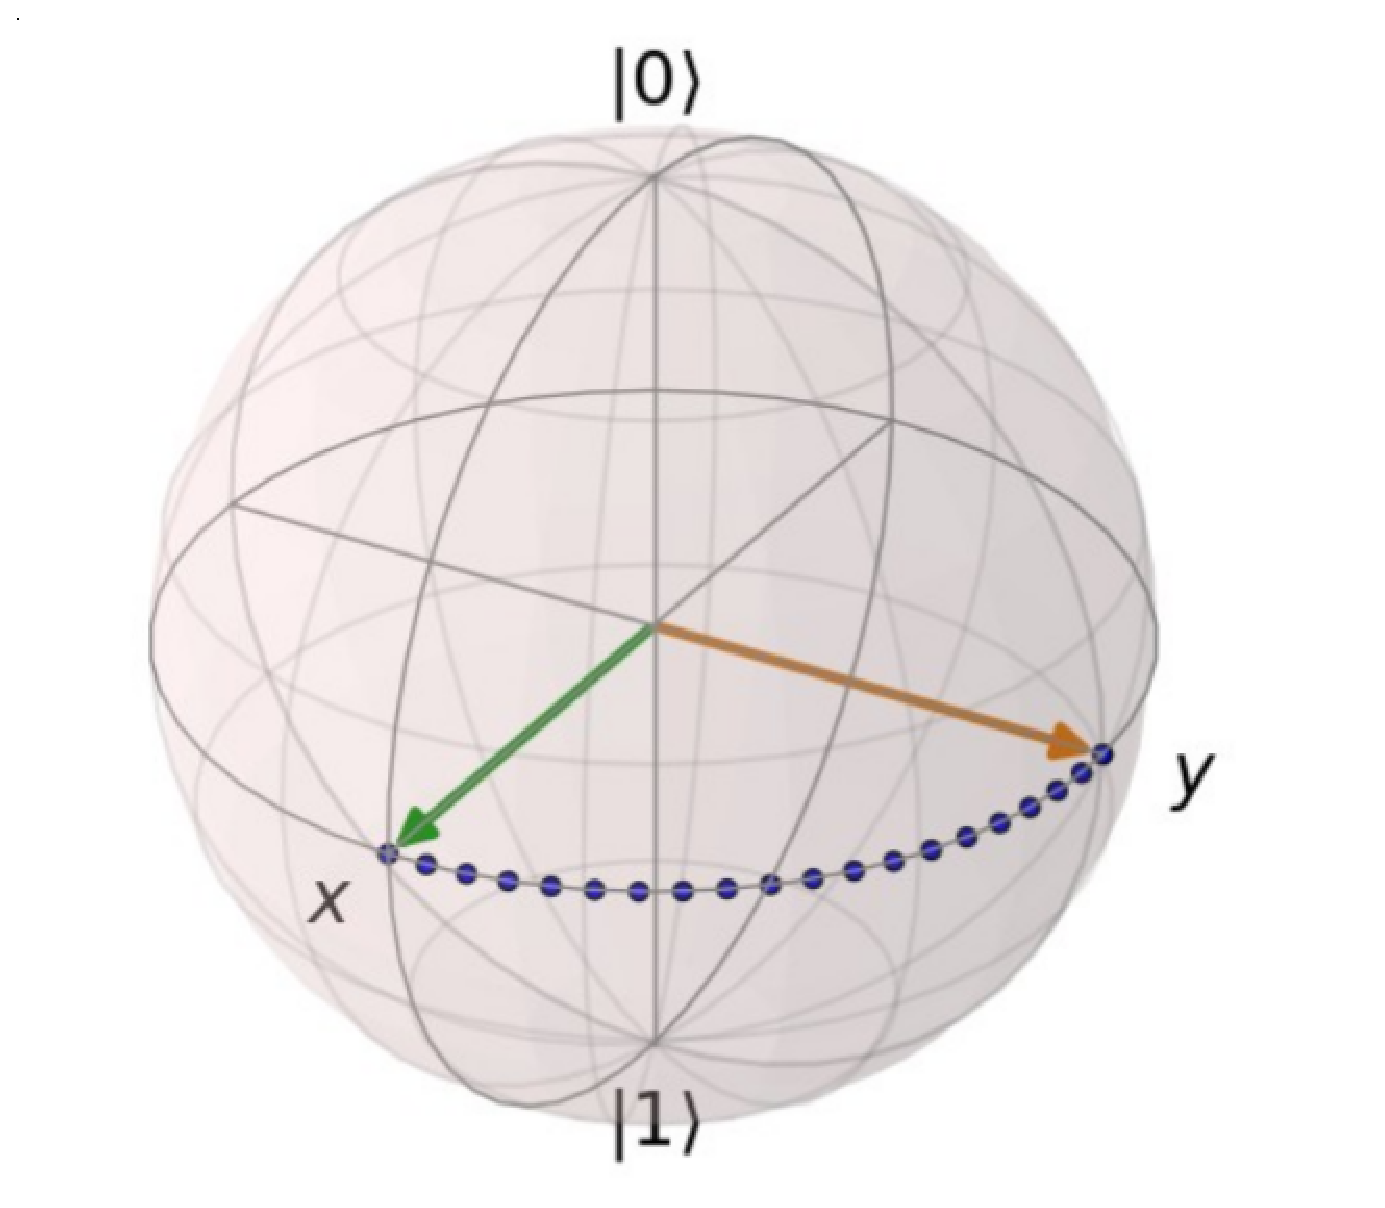
\includegraphics[scale=0.21]{s-gate.eps}
  \vspace{1mm}
  \caption{Visualización de la compuerta $S$ en la esfera de Bloch.}
  \label{fig:s_bloch}
\end{figure}


\subsection{Medida de un qubit}
En la sección (\ref{medidas}) se introdujo la idea de medida en mecánica cuántica, aquí vemos su aplicación más simple que es el caso de medir un qubit.
Al medir un qubit $\ket{\psi}$ en la base computacional, la superposición cuántica colapsa a un estado de la base. Se dice que estado $\ket{\psi}$ ``colapsó", quedando en el estado$\ket{0}$ o $\ket{1}$. Se puede calcular la probabilidad de que se obtenga cierto resultado de la medida a través de las amplitudes de probabilidad:
\begin{align}
  P(\ket{0}) &= \left|\alpha\right|^2 \\
  P(\ket{1}) &= \left|\beta\right|^2.
\end{align}

Esto se puede observar en el circuito simple de un qubit:

\begin{figure}[ht]
\begin{center}
\begin{quantikz}
\lstick{$\ket{0}$} & \gate{H} & \gate{Z} & \meter{} & \qwbundle[alternate=2]{}
\end{quantikz}
% \begin{quantikz}
% \lstick{$\ket{0}$} & \gate{H} & \gate{Z} & \meter\qwbundle[alternate=2]{} & \qwbundle[alternate=2]{} 
% \end{quantikz}
\end{center}
\caption{El resultado de la medida de un qubit es un bit clásico, que se diferencia de un qubit representándolo con un cable doble. Este circuito se puede visualizar en la esfera de Bloch en la Figura~\ref{fig:gate_rotations}.}
\end{figure}
\noindent

En primer lugar se calcula $H\ket{0} = \ket{+}$, seguido de $Z\ket{+} = (\ket{0} - \ket{1})/\sqrt 2$, (o $\ket{-}$). Finalmente se mide, obteniendo algún estado de la base computacional $\ket{j}$.
Lo único que se puede afirmar es que se obtendrá el estado $\ket{j}$ con probabilidad $|a_j|^2$:
\begin{align}
  P(\ket{0}) = \left|\dfrac{1}{\sqrt2}\right|^2 &= \dfrac{1}{2} \\
  P(\ket{1}) = \left|\dfrac{-1}{\sqrt2}\right|^2 &= \dfrac{1}{2}.
\end{align}
Teniendo igual probabilidad de medir $\ket{0}$ o $\ket{1}$.

\begin{figure}[ht]
  \centering
  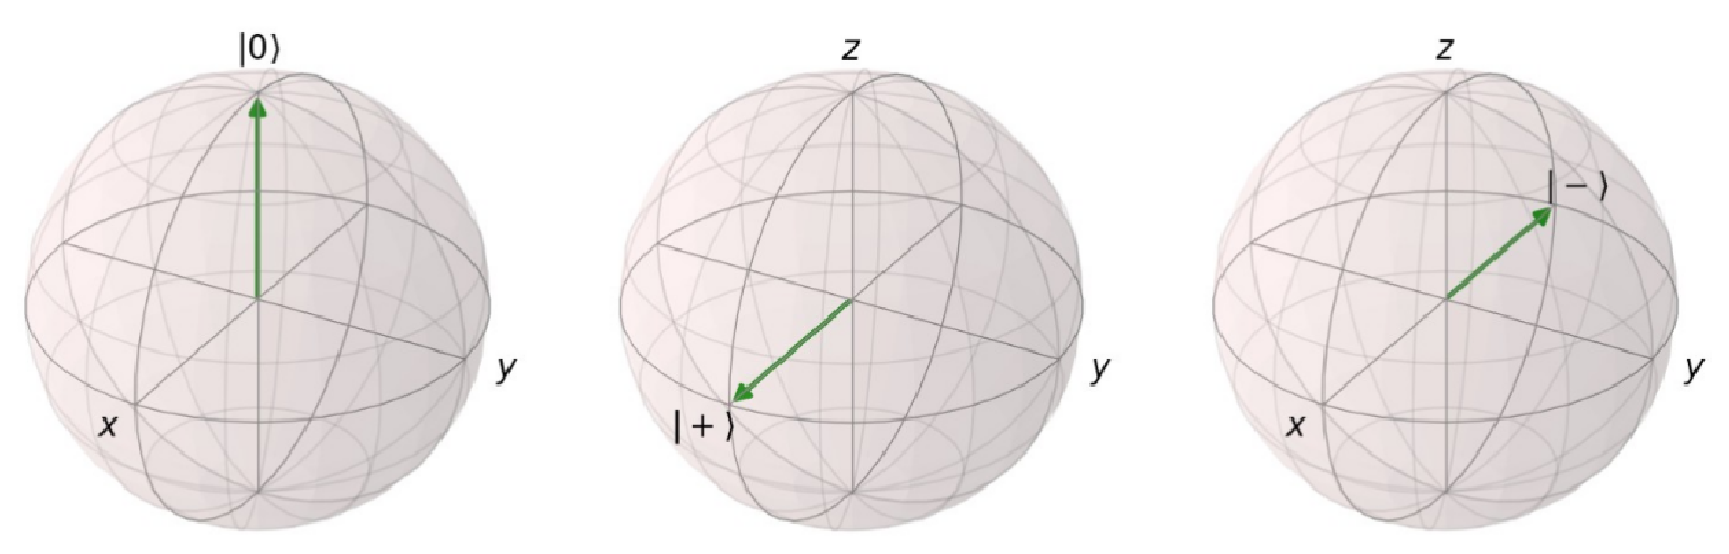
\includegraphics[scale=0.375]{simple-circuit.eps}
  \vspace{2mm}
  \caption{Estados del qubit a través del circuito: $\ket{0}$ $\rightarrow$ $H\ket{0}$ $\rightarrow$ $ZH\ket{0}$.}
  \label{fig:gate_rotations}
\end{figure}

\subsection{Notación Vectorial} \label{sec:matrix_notation}
Anteriormente vimos que un estado de un qubit se puede escribir como
\begin{equation}
  \ket{\psi} = \alpha\ket{0} + \beta\ket{1}.
\end{equation}
Los kets $\ket{0}$ y $\ket{1}$ forman la base estándar de un qubit y se representan como:
\setlength\multicolsep{0pt}
\begin{equation}
  \ket{0} = \qstatezero{}; \quad \ket{1} = \qstateone{}.
\end{equation}
\noindent
Como ya se mencionó un estado cuántico debe estar normalizado por lo que el estado de un qubit es un vector normalizado de un espacio vectorial complejo de dimensión 2. Un estado de $n$ qubits tiene un \emph{espacio de Hilbert} de dimensión $2^n$.  Un estado cuántico se puede escribir como combinación lineal de estados de la base:
\begin{equation}
  \ket{\psi} = \alpha\qstatezero{} + \beta\qstateone{} = \begin{pmatrix}\alpha \\ \beta\end{pmatrix}.
\end{equation}
Por lo que las compuertas de un qubit se pueden representar por matrices unitarias de $2 \times 2$:
\vspace*{-4mm}
\setlength\multicolsep{0pt}
\begin{multicols}{3}
  \[
    I = \igate{};
  \]
  \vfill
  \[
    X = \xgate{};
  \]
  \vfill
  \[
    Y = \ygate{};
  \]
\end{multicols}
\begin{multicols}{3}
  \[
    Z = \zgate{};
  \]
  \vfill
  \[
    S = \sgate{};
  \]
  \vfill
  \[
    H = \hgate{}.
  \]
\end{multicols}
\bigskip
\noindent
Luego, aplicar la compuerta $X$ al estado $\ket{0}$, $X \ket{0}$ se puede calcular simplemente como una multiplicación de una matriz por un vector:
\begin{equation}
  X\ket{0} = \xgate{} \qstatezero{} = \qstateone{}.
\end{equation}
Por lo que vemos que $X\ket{0} = \ket{1}$. De forma general:
\begin{equation}
  X\begin{pmatrix}\alpha \\ \beta\end{pmatrix} = \begin{pmatrix}\beta \\ \alpha\end{pmatrix}.
\end{equation}

Las compuertas cuánticas se pueden combinar multiplicando sus respectivas matrices. Por ejemplo,
podemos verificar que la compuerta Hadamard es su propia inversa:
\begin{equation}
  H^2 = \hgate{} \hgate{} = \igate{} = I.
\end{equation}
Es a su vez una \emph{matriz Hermítica}, ya que es igual a su propia transpuesta conjugada: $H = H^\dagger$.

\section{Multi-Qubits}
Para representar más de un qubit se utiliza el \emph{producto tensorial}. Dadas $A$ una matriz de  $m \times n$ y $B$ una matriz de $p \times q$, luego
\begin{equation}
  A \otimes B = \begin{pmatrix}
      a_{11} & \dots & a_{1n} \\
      \vdots & \ddots & \vdots \\
      a_{m1} & \dots & a_{mn} \\
    \end{pmatrix} \otimes B =
    \begin{pmatrix}
      a_{11}B & \dots & a_{1n}B \\
      \vdots & \ddots & \vdots \\
      a_{m1}B & \dots & a_{mn}B \\
    \end{pmatrix},
\end{equation}
resultando en un matriz de $mp \times nq$.
Se puede representar el estado de dos qubits $\ket{00}$ como
\begin{equation}
  \ket{00} = \ket{0} \otimes \ket{0} = \qstatezero{} \otimes \qstatezero{} =
  \begin{pmatrix}
    1\qstatezero{} \\[13pt]
    0\qstatezero{}
  \end{pmatrix}
  =
  \begin{pmatrix}
    1 \\
    0 \\
    0 \\
    0
  \end{pmatrix}.
\end{equation}
Las notaciones: $\ket{00} = \ket{0}\!\ket{0} = \ket{0} \otimes \ket{0}$, son equivalentes.
El estado de dos qubits se puede escribir como:
\begin{equation}
  \ket{ab} = \ket{a} \otimes \ket{b} = \alpha_{00}\ket{00} + \alpha_{01}\ket{01} + \alpha_{10}\ket{10} + \alpha_{11}\ket{11}.
\end{equation}
Un estado en general se puede escribir como combinación lineal $\sum_{j} \alpha_j\ket{\psi_j}$ de estados $\ket{\psi_j}$ con sus amplitudes correspondientes $\alpha_j$.

Notar que a diferencia de los bits clásicos, el espacio de un estado crece de forma exponencial con el número de qubits, con $n$ qubits se pueden representar $2^n$ estados. Estados de muchos qubits, como cualquier estado cuántico tienen que estar normalizado. Para un estado de $n$ qubits:
\begin{equation}
  \sum_{j = 0}^{2^n-1} |\alpha_j|^2 = 1.
\end{equation}

\subsection{Evolución de un estado de dos qubits}
En la sección (\ref{evol}) se introdujo el concepto de evolución de un sistema cuántico cerrado, en esta sección veremos un ejemplo en el caso de dos qubits en el que la unitaria es simplemente aplicarle la compuerta $H$ al segundo, $H_1\ket{0_0 0_1}$.Esto se puede obtener de forma simple:
\begin{equation}
  H_1\ket{0_0 0_1} = (I_0 \otimes H_1)\ket{0_0 0_1}.
\end{equation}
Si se quiere calcular la matriz explícitamente:
\begin{align}
  I_0 \otimes H_1 &=
  \igate{} \otimes \hgate{} \\
  &=
  \dfrac{1}{\sqrt2}
  \left[
    \igate{}
    \otimes
    \begin{pmatrix}
      1 & \phantom{-}1 \\
      1 & -1
    \end{pmatrix}
  \right] \\
&= \dfrac{1}{\sqrt2}
  \begin{pmatrix}
    1 & \phantom{-}1 & 0 & \phantom{-}0 \\
    1 & -1 & 0 & \phantom{-}0 \\
    0 & \phantom{-}0 & 1 & \phantom{-}1 \\
    0 & \phantom{-}0 & 1 & -1 \\
  \end{pmatrix}.
\end{align}
Por lo que vemos que $I_0 \otimes H_1 \ket{00}$:
\begin{equation}
  \dfrac{1}{\sqrt2}
  \begin{pmatrix}
    1 & \phantom{-}1 & 0 & \phantom{-}0 \\
    1 & -1 & 0 & \phantom{-}0 \\
    0 & \phantom{-}0 & 1 & \phantom{-}1 \\
    0 & \phantom{-}0 & 1 & -1 \\
  \end{pmatrix}
  \begin{pmatrix}
    1 \\
    0 \\
    0 \\
    0
  \end{pmatrix}
  =
  \dfrac{1}{\sqrt2}
  \begin{pmatrix}
    1 \\
    1 \\
    0 \\
    0
  \end{pmatrix},
\end{equation}
 da como resultado el estado $(\ket{00} + \ket{01})/\sqrt2=\ket{0+}$, como era de esperarse.

\subsection{Medidas parciales de dos qubits}
Ya se introdujo el concepto de medidas en la sección (\ref{medidas}), en este caso vemos un ejemplo simple de dos qubits en el que se mide el qubit $\ket{q_0}$ como se observa en el circuito:
\begin{center}
\begin{quantikz}
\lstick{$\ket{q_0} = \ket{0}$} & \gate{H} & \meter{} \\
\lstick{$\ket{q_1} = \ket{0}$} & \gate{H} & \qw \\
\end{quantikz}
\end{center}

% \[
%   \Large
%   \Qcircuit @C=1em @R=0.5em {
%     \push{\rule{0em}{1.5em}} & & & & & \lstick{\ket{q_0} = \ket{0}} & \gate{H} & \meter & \cw \\
%     \push{\rule{0em}{1.5em}} & & & & & \lstick{\ket{q_1} = \ket{0}} & \gate{H} & \qw & \qw \\
%   }
% \]
\noindent
Inicialmente los dos qubits están en el estado $\ket{00}$ y se aplica la compuerta Hadamard a cada uno:
\begin{equation}
  (H \otimes H)\ket{00} = \dfrac{1}{2}(\ket{00} + \ket{01} + \ket{10} + \ket{11}).
\end{equation}
si se mide el $\ket{q_0}$ se tiene mitad de probabilidad de obtener $\ket{0}$ o $\ket{1}$. Al medir, el estado $\ket{q_0}$ colapsa a alguno de los siguientes estados:
\begin{equation}
  \ket{\psi} =
  \begin{cases}
    \begin{aligned}
      \dfrac{1}{\sqrt2}(\ket{\uline{0}0} + \ket{\uline{0}1}) & \text{ if } M(q_0) = \ket{0} \\
      \dfrac{1}{\sqrt2}(\ket{\uline{1}0} + \ket{\uline{1}1}) & \text{ if } M(q_0) = \ket{1}
    \end{aligned}
  \end{cases}
\end{equation}
Luego de la medida se tienen dos estados posibles para $\ket{q_0}$: $\ket{0}$ o $\ket{1}$. El qubit $\ket{q_1}$ 
quedará en una superposición porque no se lo midió. Notar que los primeros qubits (subrayados) en ambos estados son iguales. Lo cual tiene sentido porque se midió este qubit por lo que se tiene certeza sobre este estado.

\section{Compuertas de dos qubits usuales}
\subsection{Compuerta CNOT}
La compuerta cuántica control-\textsc{not} (\textsc{cnot}, a veces llamada control-$X$) 
es similar a la compuerta clásica \textsc{xor}, 
pero es reversible. Esta compuerta tiene dos qubits de entrada el qubit de \emph{control} y el qubit \emph{target}. Si el qubit de control está en 0, luego se deja igual al qubit target. Pero si el qubit de control está en 1, el qubit target se invierte. El circuito que representa al \textsc{cnot} se puede observar en la  Figura~\ref{fig:cnot_circuit}. El qubit $\ket{q_0}$ representa al qubit de control y $\ket{q_1}$ representa al qubit target. Es esencialmente una compuerta $X$ con un qubit de control. \textsc{cnot} es hermítica.

\begin{figure}[ht]
  \centering
  \begin{minipage}{.45\textwidth}
   \begin{center}
   \begin{quantikz}
   \lstick{$\ket{q_0}$} & \ctrl{1} & \ctrl{1} & \qw \\
   \lstick{$\ket{q_1}$} & \targ{} & \gate{X} & \qw \\
\end{quantikz}
\end{center}
    \caption{Dos formas diferentes de representar a \textsc{cnot} en un circuito.}
    \label{fig:cnot_circuit}
  \end{minipage}%
  \hspace*{.05\textwidth}
  \begin{minipage}{.45\textwidth}
    \[
      U_{\textsc{cnot}} = \cnotgate{}
    \]
  \caption{Representación matricial de \textsc{cnot}.}
  \end{minipage}
\end{figure}
\noindent
Veamos un ejemplo en el cual se utiliza la compuerta \textsc{cnot}. 
Consideramos el siguiente circuito:

\begin{center}
   \begin{quantikz}
   \lstick{$\ket{q_0}= \ket{0}$} & \gate{X} & \ctrl{1} & \ctrl{1} & \qw \\
   \lstick{$\ket{q_1}= \ket{0}$} & \qw & \targ{} & \gate{X} & \qw \\
\end{quantikz}
\end{center}
% \[
%   \Large
%   \Qcircuit @C=1em @R=0.5em {
%     \push{\rule{0em}{1.5em}} & & & & & \lstick{\ket{q_0} = \ket{0}} & \gate{X}  & \ctrl{1} & \qw & \qw\\
%     \push{\rule{0em}{1.5em}} & & & & & \lstick{\ket{q_1} = \ket{0}} & \qw & \targ & \qw & \qw\\
%   }
% \]

En primer lugar, se aplica $X$, para poner el qubit de control $\ket{q_0}$ en el estado $\ket{1}$, obteniendo el estado  $\ket{10}$. Luego se aplica la compuerta \textsc{cnot},
\begin{equation}
  \textsc{cnot}\ket{10} = \cnotgate{}
  \begin{pmatrix}
    0 \\
    0 \\
    1 \\
    0
  \end{pmatrix}
  =
  \begin{pmatrix}
    0 \\
    0 \\
    0 \\
    1
  \end{pmatrix}
  =
  \ket{11}.
\end{equation}
Dado que se puso el qubit de control en el estado $\ket{1}$, se invierte el qubit de target, obteniendo el estado  $\ket{11}$.

\subsection{Compuerta CZ}
La compuerta \textsc{cz}, o control-$Z$ , actúa de forma similar a otras compuertas de control.
Esto es, se aplica si el qubit de control está en $\ket{1}$ y en caso contrario no hace nada.
En el caso de \textsc{cz} la operación es la compuerta $Z$, la compuerta \textsc{cz} también es hermítica.

\begin{figure}[ht]
  \begin{center}
   \begin{quantikz}
   \lstick{$\ket{q_0}$} & \ctrl{1} & \qw & \ctrl{1} & \qw \\
   \lstick{$\ket{q_1}$}  & \ctrl{-1} & \qw & \gate{Z} & \qw  \\
\end{quantikz}
\end{center}
\caption{Dos formas diferentes de representar a \textsc{CZ} en un circuito.}
\end{figure}


% \begin{figure}[ht]
%   \[
%     \Large
%     \Qcircuit @C=1em @R=0.5em {
%       \push{\rule{0em}{1em}} & & \lstick{\ket{q_0}} & \ctrl{1} & \qw & \ctrl{1} & \qw \\
%       \push{\rule{0em}{1em}} & & \lstick{\ket{q_1}} & \ctrl{-1} & \qw & \gate{Z} & \qw  \\
%     }
%   \]
% \caption{Dos formas diferentes de representar a \textsc{CZ} en un circuito.}
% \end{figure}

\subsection{Compuertas de Control}
Las Compuertas de Control actúan en dos o más qubits, en las cuales uno o más qubits actúan como control para cierta operación. Generalmente, si $U$ es una compuerta que opera sobre qubits individuales tiene una representación matricial:
\begin{equation}
  U =
  \begin{pmatrix}
    u_{00} & u_{01} \\
    u_{10} & u_{11} \\
  \end{pmatrix},
\end{equation}
luego la compuerta control-$U$ en la que el 
qubit de control es el 0 y el target el 1, tiene la siguiente representación matricial:
\begin{equation}
  C_U =
  \begin{pmatrix}
    1 & 0 & 0 & 0 \\
    0 & 1 & 0 & 0 \\
    0 & 0 & u_{00} & u_{01} \\
    0 & 0 & u_{10} & u_{11} \\
  \end{pmatrix}.
\end{equation}
\section{Compuerta Toffoli}
La compuerta Toffoli tiene tres entradas y salidas (Figura \ref{fig:toffoli_circuit}), donde dos de los qubits de entrada actúan como control. El tercer qubit es el target que se invierte cuando ambos qubits de control están en $\ket{1}$, 
en caso contrario no se le hace nada. Por ejemplo, si se aplica la compuerta Toffoli al estado $\ket{110}$,
se invierte el tercer qubit, por lo que se obtiene el estado $\ket{111}$.


\begin{figure}[ht]
  \begin{center}
   \begin{quantikz}
        \lstick{$\ket{x}$} & \ctrl{1} & \qw & \rstick{\hspace*{-3mm}$\ket{x}$} \\
        \lstick{$\ket{y}$} & \ctrl{1} & \qw & \rstick{\hspace*{-3mm}$\ket{y}$} \\
        \lstick{$\ket{z}$} & \targ & \qw & \rstick{\hspace*{-3mm}$\ket{z \oplus (x \land y)}$}\\
    \end{quantikz}
\end{center}
\caption{Circuito que representa la compuerta Toffoli, donde $\oplus$ es la suma binaria (\textsc{xor}).}
  \label{fig:toffoli_circuit}
\end{figure}
\noindent

% \begin{figure}[ht]
%   \[
%     \Large
%     \Qcircuit @C=0.54em @R=1em {
%       \push{\rule{0em}{1em}} & & & \lstick{\ket{x}} & \ctrl{1} & \qw & \rstick{\hspace*{-3mm}\ket{x}} \\
%       \push{\rule{0em}{1em}} & & & \lstick{\ket{y}} & \ctrl{1} & \qw & \rstick{\hspace*{-3mm}\ket{y}} \\
%       \push{\rule{0em}{1em}} & & & \lstick{\ket{z}} & \targ & \qw & \rstick{\hspace*{-3mm}\ket{z \oplus (x \land y)}}\\
%     }
%   \]
%   \caption{Circuito que representa la compuerta Toffoli, donde $\oplus$ es la suma binaria (\textsc{xor}).}
%   \label{fig:toffoli_circuit}
% \end{figure}
% \noindent

La compuerta Toffoli, o control-control-X (\textsc{ccx}) se puede representar por una
matriz de $8 \times 8$:
\begin{equation}
  U_{CCX} =
  \begin{pmatrix}
    1 & 0 & 0 & 0 & 0 & 0 & 0 & 0\\
    0 & 1 & 0 & 0 & 0 & 0 & 0 & 0\\
    0 & 0 & 1 & 0 & 0 & 0 & 0 & 0\\
    0 & 0 & 0 & 1 & 0 & 0 & 0 & 0\\
    0 & 0 & 0 & 0 & 1 & 0 & 0 & 0\\
    0 & 0 & 0 & 0 & 0 & 1 & 0 & 0\\
    0 & 0 & 0 & 0 & 0 & 0 & 0 & 1\\
    0 & 0 & 0 & 0 & 0 & 0 & 1 & 0\\
  \end{pmatrix}.
\end{equation}

 %\section{Conjunto de Compuertas Universales} \label{sec:universal_gate_sets}

%%%%%%%%%Conviene completar con lo que se dio en clase de como generar gates

% In classical systems the \textsc{nand} gate is a universal gate, meaning that any other gate can be represented as a combination of \textsc{nand} gates. In quantum computing there exist universal gate sets. A universal gate set requires the full Clifford and Pauli groups, and one or more non-Clifford gates.

% We've seen the Pauli gates in Section \ref{pauli_gates}. On their own, Pauli gates have no interesting computational capabilities. The Clifford gates we have seen are $H$, $S$, \textsc{cnot} and \textsc{cz}. Clifford gates introduce the quantum phenomena superposition and entanglement. The Pauli and Clifford gates can be simulated efficiently by classical computers (\emph{Gottesman-Knill theorem}) - showing no increase in efficiency over classical computers.

% The non-Clifford gates, which are required for universal quantum computing, cannot be simulated efficiently and are exponentially hard to simulate. Some non-Clifford gates are Toffoli, $T$ and the rotation gates $R_x$, $R_y$ and $R_z$ (which do arbitrary rotations around the axes). One universal gate set that allows universal quantum computing is $\{H,\, T,\, \textsc{cnot}\}$.


\chapter{Entrelazamiento Cuántico}

\begin{center}
  \begin{minipage}{0.5\textwidth}
    \begin{small}
      `` Solo sé que no sé nada y, al saber que nada sé, algo sé.'' \par
%\setlength{\parindent}{30ex}
 \begin{flushright}{\it Sócrates}
 \end{flushright}
    \end{small}
\end{minipage}
  \vspace{0.5cm}
\end{center}

Una propiedad clave que caracteriza el comportamiento de los sistemas en el régimen cuántico es el llamado 
\emph{Entrelazamiento cuántico}. Esta propiedad puede entenderse como la imposibilidad de representar las correlaciones existentes en un sistema
cuántico en términos de una distribución estadística sobre posibles configuraciones del sistema, especificables en términos de estados locales definidos.
Para entender cómo esta noción es fundamental en la descripción clásica de los sistemas físicos, consideremos por ejemplo el sistema Tierra-Luna-Sol.
Para la mecánica newtoniana, estos tres astros son entes distintos, con propiedades independientes. Así, en cada instante el Sol, la Tierra y la Luna 
cuentan con posiciones y velocidades bien definidas. El efecto de la interacción entre estos cuerpos se reduce entonces a cambiar las velocidades de 
estos cuerpos en función de las posiciones de los otros. Este marco de trabajo, que podemos llamar \emph{reduccionista}, permite describir y predecir
el comportamiento de la mayoría de los sistemas físicos macroscópicos en forma a la vez computacionalmente eficiente y precisa. Sin embargo, al tratar
de aplicarlo a sistemas en la escala atómica comienza a mostrar sus fallas: en esta escala, el entrelazamiento implica que para ciertos estados 
del sistema, las propiedades de las partes no estén bien definidas. Por ejemplo, el estado típico de una molécula de Hidrógeno no puede en general 
describirse en términos de los estados de los átomos que la conforman: existen observables globales (la energía de la molécula, el impulso angular) 
que no son  compatibles con los observables asociados a los átomos por separado. Esto nos obliga en mecánica cuántica a tratar los sistemas compuestos 
desde una perspectiva \emph{holística}, en el sentido de que debemos tratar al sistema como un todo. Una consecuencia inmediata es que la descripción exacta 
de los sistemas cuánticos se vuelve mucho más compleja que la de su equivalente clásico.

Sin embargo, no todos los sistemas cuánticos parecen requerir de una descripción que aborde toda esa complejidad potencial. Por ejemplo, el sistema 
Tierra-Sol-Luna en sí es un sistema cuántico. La clave del éxito de su descripción clásica consiste en que en su evolución el estado de cada una de
sus partes permanece bien definido. Decimos entonces que el sistema admite descripción en términos de  \emph{estados separables}. Por otro lado, la 
molécula de Hidrógeno típicamente se encuentra en un estado en el que el estado de sus partes no está bien definido. Decimos por esto que su descripción
requiere considerar \emph{estados entrelazados}.  Podemos decir entonces que cuanto más entrelazados se encuentren los estados típicos de un sistema 
(en un dado régimen) más nos costará representarlos en forma precisa y eficiente a la vez.

%Si bien la definición de entrelazamiento no parece ofrecer grandes dificultades, 
La definición y evaluación
de medidas que cuantifiquen el grado de entrelazamiento presente en un sistema es una tarea bastante más compleja, tanto desde un punto de vista formal 
como práctico. En lo que resta del capítulo daremos una definición más formal de lo que es un  \emph{estado cuántico entrelazado} \cite{NC.00,V.07,Sch1,BDSW.96}. 
Se introducirán entonces algunos elementos de la teoría de la información que nos permitirán definir medidas de entrelazamiento y de correlaciones cuánticas entre
 partes de un sistema.
 
%  En los capítulos siguientes, utilizaremos estas cantidades para estudiar algunos aspectos del comportamiento cadenas de espines en el régimen cuántico, 
% % así como para analizar la aplicabilidad de la aproximación de \emph{Campo Medio Generalizado} para su descripción.

\section{Operador Densidad y Entropía de Von Neumann}
%Nos interesa ahora extender las definiciones previas a sistemas cuánticos
%\cite{NC.00,V.07}.  
%nte destacar desde el principio que no todas las
%extensiones posibles son necesariamente triviales, y que no todas las desigualdades anteriores
%continuarán siendo v\'alidas.
El estado de un sistema cuántico 
%que cuyos estados pertenecen a un espacio de Hilbert de dimensión finita $n$
se puede caracterizar por un {\it operador densidad} (o
matriz densidad) $\rho$, el cual es un operador hermítico de traza 1 y con todos sus autovalores no negativos:
\begin{equation}\rho\geq 0\,,\;\;{\mathrm Tr}\rho=1\,.\end{equation}
Este operador determina el valor medio de cualquier observable $O$: 
% se puede determinar de la formaexpresi\'on
%Recordemos que el valor medio de cualquier observable $O$ est\'a dado por
\begin{equation}\langle O\rangle={\rm Tr}\,\rho\,O\,.\end{equation}
La probabilidad de encontrar al sistema en un estado particular $|i\rangle$,
(que supondremos normalizado) es entonces
\begin{equation}
p_i=\langle P_i\rangle={\rm Tr}\,\rho\,P_i=\langle i|\rho|i\rangle\,,
\end{equation}
donde $P_i=|i\rangle \langle i|$ es el proyector ortogonal sobre el estado $|i\rangle$.
%Recordemos tambi\'en que si la descomposici\'on espectral de $O$ es $O=\sum_\nu    o_\nu|\nu\rangle\langle\nu|$,
%la probabilidad de medir el valor $o_\nu$ ser\'a, asumiendo este no degenerado,
%\[p_{\nu}=\langle \nu|\rho|\nu\rangle\,.\]
%En el caso general,
%\[p_{o_\nu}={\rm Tr}\rho\,P_{p_\nu}\]
%siendo $P_{o_\nu}$ el proyector ortogonal sobre el autoespacio asociado. % al autovalor $o_\nu$.

En el caso de un sistema cuántico en un estado puro
$|i\rangle$, $\rho$ es entonces el proyector ortogonal sobre el espacio generado por $|i\rangle$:
\begin{equation}\rho=|i\rangle\langle i|\,,
\end{equation}
y satisface $\rho^2=\rho$. En el caso general, la descomposición espectral de $\rho$ la escribiremos como
%$\rho^2\leq\rho$ (es decir,
%$\rho-\rho^2$ es un operador positivo).
\begin{equation}\rho=\sum_i p_i|i\rangle\langle i|\,,\end{equation}
donde $\{p_i,i=1,\ldots,n\}$ %con $n$ la dimensi\'on del espacio,
son los autovalores de $\rho$ ($p_i\geq 0$, $\sum_i p_i=1$) y $\{|i\rangle,i=1,\ldots,n\}$ los
correspondientes autovectores normalizados ($\langle i|i'\rangle=\delta_{ii'}$). El caso puro corresponde a $p_i=1$ para un cierto estado y 0 para todos los demás.
En el caso general, tenemos $\rho^2\leq \rho$ (es decir, $\rho^2-\rho$ es un
operador con autovalores $-p_i(1-p_i)$ negativos o nulos).

%Recordemos que el valor medio de cualquier observable $O$ esta dado por
La entropía de von Neumann\cite{NC.00,Wh,vn.27} se define como
\begin{eqnarray}S(\rho)&=&-{\rm Tr}\,\rho\log\rho\\&=&
-\sum_i p_i\log p_i\,,\end{eqnarray}
y es una medida de la falta de información asociada al estado $\rho$. Tenemos $S(\rho)\geq 0$, con $S(\rho)=0$ únicamente 
si $\rho$ es un estado puro ($\rho^2=\rho$).
$S(\rho)$ será por el contrario máxima ($S(\rho)=\log n$ si el espacio de Hilbert del sistema tiene dimensión $n$) si el estado $\rho$ es máximamente ``mezclado''
$\rho_n=I_n/n$, donde $I_n$ denota el operador identidad, tal que $p_i=1/n$ $\forall$ $i$.

\section{Sistemas Compuestos y Estados Reducidos}

Dados dos sistemas cuánticos distinguibles, que denotaremos como $A$ y $B$, con sendos espacios de Hilbert $\mathcal{H}_A$ y $\mathcal{H}_B$ 
y espacio de Hilbert conjunto $\mathcal{H}_A\otimes \mathcal{H}_B$, el estado conjunto estará determinado por una cierta {\it 
matriz densidad conjunta} $\rho_{AB}$. La entropía conjunta es por lo tanto
\begin{equation}S(A,B)=S(\rho_{AB})=-{\rm Tr}\,\rho_{AB}\log \rho_{AB}\,.
 \label{SAB}\end{equation}
%Tenemos en mente, como caso t\'{\i}pico, dos sistemas distinguibles $A$, $B$
%espacialmente separados,  aunque las siguientes expresiones son v\'alidas para
%todo par $A$, $B$ con espacio conjunto accesible $H_A\otimes H_B$. 
Un observable {\it local} en el sistema $A$ es un observable de la forma
$O_A\equiv O_A\otimes I_B$, donde $I_B$ denota la identidad en $\mathcal{H}_B$. Su valor
medio es entonces
\begin{eqnarray}
\langle O_A\rangle&=&{\rm Tr}\,\rho_{AB}O_A%\nonumber\\
={\rm Tr}_A\, \rho_A O_A\,,
\end{eqnarray}
donde hemos definido la {\it matriz densidad reducida} \cite{NC.00,Wh}
\begin{equation}
 \rho_A={\rm Tr}_B\,\rho_{AB}\label{rhoa}\,\end{equation}
la cual determina completamente los valores medios de todo observable local en $A$.
Explícitamente, $\langle i|\rho_A|j\rangle=\sum_k\langle ik|
\rho_{AB}|jk\rangle$, donde $|ik\rangle\equiv|i\rangle\otimes|k\rangle$ son
los estados de una base producto ortonormal de $\mathcal{H}_A\otimes \mathcal{H}_B$. Análogamente,
\[\rho_B={\rm Tr}_A\,\rho_{AB}\,,\]
determina los valores medios de cualquier operador local $O_B$ en $B$. Las
entropías locales son
\[S(A)=-{\rm Tr}\,\rho_A\log\rho_A\,,\;\;\;
 S(B)=-{\rm Tr}\,\rho_B\log\rho_B\,.\]
El estado conjunto es no correlacionado si y solo si $\rho_{AB}=\rho_A\otimes
\rho_B$, es decir, si y solo si es un estado producto, en cuyo caso
sus autovalores son $p_{ij}=p_i^A p_j^B$ con $p_i^A$ y $p_j^B$ 
los autovalores de $\rho_A$ y $\rho_B$ respectivamente.  
%es decir, si est\'a completamente determinado por los operadores
%densidad reducidos (o sea, por observaciones locales), en cuyo caso 
%Esto corresponde al caso
%de  v.a.\ independientes en sistemas clásicos.
En tal caso las entropías
satisfacen $S(A,B)=S(A)+S(B)$, como es fácil ver de la
definición (\ref{SAB}).
\section{Información  Mutua y Entropía Condicional}

%Podemos definir ahora la {\bf entropía condicional} utilizando la %f\'ormula\cite{NC.00,Wh,OZ.01}:
%\begin{eqnarray}S_1(A|B)&\equiv&S(A,B)-S(B)\label{qcond1}\\
% &=&S(\rho_{AB})-S(\rho_B)\,.\label{qcond11}\end{eqnarray}
%No obstante, es fundamental notar que esta cantidad {\it 
%no es necesariamente positiva}. Es decir, la entrop\'{\i}a global
%$S(A,B)$ puede ser {\it mayor}, pero también {\it menor} que las entrop\'{\i}as locales.
%El caso menor se da en los estados {\it entrelazados}, que definiremos en detalle
%en el pr\'oximo cap\'{\i}tulo, y del cual se dar\'a  un ejemplo en este cap\'{\i}tulo.

%La segunda versión cuántica de la entropía condicional fue introducida por
%Zurek en 2001 \cite{Zu1.01} y la discutiremos en el cap\'{\i}tulo 4 cuando describamos el {\it Quantum Discord}.
% ({\it Discordancia Cuántica}).

%En base a $S_1(X|Y)$, podemos definir la primera versión c\'uantica de
Podemos ahora definir la {\bf información mutua} como % siguiendo las ecuaciones (\ref{mut1})--(\ref{mut2}):
\begin{eqnarray}
I(A:B)&=&S(\rho_A)+S(\rho_B)-S(\rho_{AB})\,.\label{qmut1}%\\
%&=&S(A)-S_1(A|B)=S(B)-S_1(B|A)\label{qmut0}\\
%&=&S(A)+S(B)-S(A,B)
\end{eqnarray}
Esta cantidad es una medida de la correlación (total) entre $A$ y $B$
\cite{NC.00,Wh}. Si $\rho_{AB}=\rho_A\otimes\rho_B$, %$A$ y $B$ son no correlacionados,
$S(\rho_{AB})=S(\rho_A)+S(\rho_B)$ y por lo tanto $I(A:B)=0$. En caso contrario 
$I(A:B)>0$. 

%A diferencia de $S_1(A|B)$, $S_1(A:B)$ es {\it positiva}: $S_1(A:B)\geq 0$. % tal como se demuestra en el ap\'endice. 
Esta positividad de $I(A:B)$ es conceptualmente evidente: $S(A)+S(B)$ es una medida de la falta de
información cuando s\'olo se dispone de información sobre los valores medios de todos los observables locales (es decir, cuando se conoce s\'olo $\rho_A$ y $\rho_B$), 
 mientras que $S(A,B)$ mide la falta de información cuando se conoce además
toda la información sobre las correlaciones,
es decir, sobre todos los valores medios de observables generales del tipo $O_{AB}=O_A\otimes O_B$. Por lo tanto $S(A,B)\leq S(A)+S(B)$.

Clásicamente, es decir, para sistemas descriptos por densidades de probabilidad, se tiene además 
\begin{equation}
S(A,B)\geq S(A),\;\;\;S(A,B)\geq S(B)\label{desc}\end{equation}
Las entropías condicionales $S(A|B)$ y $S(B|A)$ pueden definirse como 
\begin{equation}S(A|B)=S(A,B)-S(B),\;\;S(B|A)=S(A,B)-S(A)\label{Scond}\end{equation}
y son por lo tanto cantidades no negativas en sistemas clásicos. 
%Podemos as\'{\i} reescribir la informaci\'on mutua como 

Sin embargo, la desigualdad (\ref{desc}) no sigue siendo válida en sistemas cuánticos, es decir, en sistemas descriptos por operadores densidad. En otras palabras, en sistemas cuánticos la entropía global puede ser menor que las entropías locales, y las entropías condicionales definidas como en (\ref{Scond}) pueden por lo tanto ser negativas. 


A modo de ejemplo, consideremos un par de qubits o espines $1/2$
en un estado de Bell, por ejemplo
\begin{equation}|\Psi\rangle=\frac{|\!\!\uparrow\uparrow\rangle+
|\!\!\downarrow\downarrow\rangle}{\sqrt{2}}
 \label{bell1}\,,\end{equation}
donde $|\!\!\uparrow\uparrow\rangle=|\!\!\uparrow\rangle\otimes|\!\!\uparrow\rangle$
denota un estado con ambos espines en la dirección $z$ positiva. 
%Este estado
%lo reescribiremos, siguiendo la notación acostumbrada en información cuántica,
%como
% \begin{equation}|\Psi\rangle=\frac{|00\rangle+|11\rangle}{\sqrt{2}}\,.
% \label{bell2}\end{equation}
El estado $\rho=|\Psi\rangle\langle\Psi|$ es un estado puro y por lo tanto, 
%Para este estado, obviamente 
\[S(\rho_{AB})=0\,.\] 
%(pues $\rho_{AB}=|\Psi\rangle\langle\Psi|$
%orresponde a un estado puro ($\rho_{AB}^2=\rho_{AB}$))
No obstante, los estados reducidos son máximamente mezclados: 
\[\rho_A=\rho_B=\frac{1}{2}I_2=\frac{1}{2}(|\uparrow\rangle\langle \uparrow|+|\downarrow\rangle\langle \downarrow|)\,.\]
%es decir, las matrices densidad reducidas est\'an m\'aximamente mezcladas
Por lo tanto,
\begin{equation}
S(\rho_A)=S(\rho_B)=1\,,\end{equation}
tomando el logaritmo en base $2$.  Esto implica $S(A)=S(B)>S(A,B)=0$, a diferencia de cualquier sistema clásico. M\'as aun, los estados locales están máximamente mezclados (es decir, máximamente ``desordenados'') a pesar de  que el estado global es puro (es decir, máximamente ``ordenado''). Para este estado tenemos entonces 
\[I(A:B)=2\]
\[S(A|B)=S(B|A)=-1\,.\]
Como veremos a continuación, la violación de las desigualdades clásicas (\ref{desc}) puede darse solo cuando el estado $\rho$ es entrelazado. 

%Este estado es un estado máximamente entrelazado de dos qubits, en el que el
%sistema conjunto está ``máximamente ordenado'' (está en un estado puro) pero el
%sistema local está máximamente desordenado. %Esto es imposible en el caso cl\'asico, ya que si $p_{ij}=1$ para un cierto par $(i,j)$ (y 0 para los restantes) entonces
%necesariamente $p^A_i=p^B_j=1$ y entonces $S(A)=S(B)=0$.
%Este estado conduce pues a un caso
%extremo de no extensividad: Mientras que $S(A)=S(B)=1$, la entropía global $S(A,B)$, lejos de ser
%igual a la suma, es {\bf nula}.

%Puede tambi\'en afirmarse que el estado de Bell corresponde a un caso de correlaci\'on extremo,
%sin an\'alogo cl\'asico, en el que
%\[S_1(A:B)=S(A)+S(B)-0=2\]
%En el caso de dos sistemas cl\'asicos binarios, el valor m\'aximo de $S(A:B)$ es 1 y
%corresponde a $p_{ij}=\delta_{ij}/2$, es decir a un sistema en el que ambos estan o bien
%en el estado $0$, o bien en el estado $1$, con igual probabilidad.

%Finalmente, mencionemos que todo el formalismo estadístico clásico se recupera
%como caso particular del cuántico si nos restringimos a operadores densidad
%conjuntos de la forma
%\begin{equation}\rho=\sum_{i,j}p_{ij}|ij\rangle\langle ij|
%\label{rhoclas}\end{equation}
%es decir, diagonales en una base
%producto $\{|ij\rangle=|i\rangle\otimes|j\rangle$\},
%y a observables que son diagonales en esta base (y por lo tanto conmutantes y simult\'aneamente medibles).
%En este caso,
%las matrices densidad reducidas son $\rho_A=\sum_{i}p_i^A|i\rangle\langle i|$,
%$\rho_B=\sum_j p_j^B|j\rangle\langle j|$ y quedan completamente determinadas
%por las distribuciones marginales $p_i^A=\sum_j p_{ij}$,
%$p_j^B=\sum_i p_{ij}$, como en el primer cap\'{\i}tulo. Los valores medios de
%observables diagonales $O_{AB}$, $O_A$ y $O_B$ son pues determinados puramente
%por la distribuciones $p_{ij}$, $p^A_{i}$ y $p^B_{i}$
%respectivamente.

%\section{Apéndice} Demostremos que la entropía mutua cuántica es también positiva
%\cite{Wh}:
%\[S_1(A:B)\geq 0\,,\]
%con $S_1(A:B)=0$ si y solo si $\rho_{AB}=\rho_A\otimes\rho_B$. \\
%Utilizando la misma propiedad anterior del logaritmo, y escribiendo
%\[\rho_{AB}=\sum_\nu p_\nu|\nu\rangle\langle\nu|,  \;\;
%\rho_A%={\rm Tr}_B\,\rho_{AB}
%=\sum_{i} p_i^A|i\rangle\langle i|\,,\;\;
%\rho_B%={\rm Tr}_A\,\rho_{AB}
%=\sum_{j} p_j^B|j\rangle\langle j|\,,\]
%con $p_i^A=\sum_{\nu,j}p_\nu|\langle ij|\nu\rangle|^2\,,
%\;\;p_j^B=\sum_{\nu,i}p_\nu|\langle ij|\nu\rangle|^2\,,$
%y $|ij\rangle=|i\rangle\otimes |j\rangle$ los estados de una base producto
%ortonormal formada por los autoestados de $\rho_A$ y $\rho_B$, se tiene,
%utilizando nuevamente  que
% $\log x\leq x-1$,
%\[S_1(A:B)=-\sum_{i,j,\nu}p_\nu|\langle ij|\nu\rangle|^2\log\frac{p_i^A p_j^B}{p_\nu}
%\geq \sum_{i,j,\nu}p_\nu|\langle ij|\nu\rangle|^2(\frac{p_i^A p_j^B}{p_\nu}-1)
% =1-1=0\]
%donde la igualdad se cumple solo si $p_i^A p_j^B=p_\nu$ para algún $\nu$
%$\forall$  $i,j$, es decir si $p_\nu=p_i^A\,p_j^B$ con
%$|\nu\rangle=|ij\rangle$.

\section{Entrelazamiento de Estados Puros}
Si un estado cuántico puro $|\Psi_{AB}\rangle$ de un sistema conjunto $A+B$ se puede escribir como
estado producto, no posee entrelazamiento y se lo denomina  {\it separable}. Por otro lado un estado {\it entrelazado} no puede descomponerse en un producto de estados: 
\begin{eqnarray}|\Psi_{AB}\rangle=|\Psi_A\rangle|\Psi_B\rangle&\Rightarrow&|\Psi_{AB}\rangle\;separable\\
 |\Psi_{AB}\rangle\neq |\Psi_A\rangle|\Psi_B\rangle&\Rightarrow&|\Psi_{AB}\rangle\; entrelazado
 \label{QE1}\end{eqnarray}
Las entropías de los subsistemas de un estado puro son idénticas (v\'ease (\ref{rred}) y permiten definir la {\it entropía de entrelazamiento} \cite{NC.00,Sch1},  que cuantifica el {\bf entrelazamiento} de un estado cuántico puro bipartito, como 
\begin{equation}E(A,B)=S(A)=S(B)\,.\label{EAB}\end{equation}
$E(A,B)$ es una medida de las correlaciones
cuánticas en el estado. Si $|\Psi_{AB}\rangle$ es separable, entonces $\rho_A=|\Psi_A\rangle\langle
\Psi_A|$, $\rho_B=|\Psi_B\rangle\langle\Psi_B|$ y $E(A,B)=0$.

En el caso puro $E(A,B)$ es menos la entropía condicional:
\begin{equation}S(A|B)=S(B|A)=-E(A,B)\,,\end{equation}
pues $S(A,B)=0$. Mientras que la correspondiente información mutua es
\begin{equation}I(A:B)=S(A)-S(A|B)=2S(A)=2E(A,B)\,.\end{equation}
Podemos considerar a $I(A:B)$ como una medida de todas las correlaciones
en el sistema, mientras que a $E(A,B)$ como una medida de correlaciones
puramente cuánticas.

Una forma de determinar si un estado cuántico es entrelazado es a través de la
{\it descomposición de Schmidt} del estado \cite{NC.00}:
Existen siempre bases locales $\{|k_A\rangle\}$ y $\{|k_B\rangle\}$
ortonormales, en las que $|\Psi\rangle$ puede escribirse en la forma
\begin{equation}|\Psi\rangle=\sum_{k=1}^{n_s} \sigma_k|k_A\rangle|k_B\rangle
\,,\label{SD}
\end{equation}
donde $n_s$ es el número de Schmidt y $\sigma_k>0$,
$\sum_{k=1}^{n_s}\sigma_k^2=1$. Las matrices densidad
reducidas están entonces dadas por
\begin{equation}\rho_A=\sum_{k} \sigma_k^2|k_A\rangle\langle k_A|\,,\;\;
\rho_B=\sum_{k} \sigma_k^2|k_B\rangle\langle k_B|\label{rred}\,.\end{equation}
Estas son isospectrales por lo que $S(A)=S(B)$.
%\begin{eqnarray}\rho_A&=&{\rm Tr}_B |\Psi\rangle\langle\Psi|
%=\sum_{k} \sigma_k^2|k_A\rangle\langle k_A|,\\
%\rho_B&=&{\rm Tr}_A |\Psi\rangle\langle\Psi|
% =\sum_{k}\sigma_k^2|k_B\rangle\langle k_B|\,,\end{eqnarray}
%siendo pues estas bases locales (denominadas bases de Schmidt) justamente las
%que diagonalizan los operadores densidad reducidos. Estos son pues siempre
%isospectrales, implicando $S(A)=S(B)$.
El caso separable corresponde a $n_s=1$,
donde  $E(A,B)=0$, mientras que el caso entrelazado a $n_s\geq 2$, en el que
\begin{equation}E(A,B)=-\sum_{k=1}^{n_s}\sigma_k^2\log (\sigma_k^2)
\label{EAB2}
\end{equation}
La descomposición de Schmidt puede obtenerse a partir de la
{\itshape descomposición en valores singulares} de la matriz de los coeficientes
de expansión de $|\Psi\rangle$ en una base producto ortogonal, arbitraria
\cite{NC.00}, siendo los $\sigma_k$ los valores singulares de dicha matriz.
En el caso del estado de Bell (ecuación \ref{bell1}), ya está
expresado en una base de Schmidt, con $n_s=2$ y
$\sigma_1=\sigma_2=1/\sqrt{2}$. 

El entrelazamiento es considerado un {\it recurso
esencial} en información cuántica \cite{NC.00,V.07}, ya que permite formas
radicalmente nuevas de intercambio y procesamiento de la información,
tales como la teleportación cuántica \cite{t.93} y la computación cuántica \cite{NC.00}. 
% imposibles de simular eficientemente en sistemas clásicos.

\section{Entrelazamiento de Estados no Puros}
La definición de entrelazamiento cuántico es m\'as compleja para estados $\rho$ generales 
no necesariamente puros ($\rho^2\leq\rho$). De hecho, en el caso general no es posible obtener un m\'etodo general 
para determinar si el estado es entrelazado, en un n\'umero finito de pasos. Por lo tanto tampoco es posible
obtener una medida computable del mismo.

%entrelazamiento, e incluso, no est\'a a\'un resuelto el problema formal
%de definir una medida de todas las correlaciones cuánticas en estados no puros.

Según la definición introducida por R.F. Werner en 1989 \cite{W.89}, un estado
cuántico general es {\it entrelazado} si no es {\it separable} o {\it clásicamente correlacionado}, 
en cuyo caso puede ser escrito como una combinación convexa de estados producto, es decir,
una superposición estadística de estados no correlacionados:
\begin{eqnarray}\rho=\sum_{\alpha} q_\alpha \rho_A^\alpha\otimes\rho_B^\alpha,
\;\;q_\alpha\geq 0,\;&\Rightarrow & \rho\;separable\label{rs2}\\
\rho\neq \sum_{\alpha} q_\alpha \rho_A^\alpha\otimes\rho_B^\alpha,
 \;\;q_\alpha\geq 0,&\Rightarrow& \rho\;entrelazado\end{eqnarray}
donde $\sum_\alpha q_\alpha=1$. En particular, un estado producto
$\rho_{AB}=\rho_A\otimes\rho_B$, es decir, un estado no correlacionado, es un
estado separable. Pero también lo es cualquier combinación convexa de los
mismos. El argumento \cite{W.89} es que los estados separables pueden ser
generados mediante operaciones locales y comunicación clásica (es decir, por
({\it LOCC: Local Operations and Classical Communication}) \cite{NC.00}) y por lo tanto no
contienen correlaciones cuánticas.
`
En otras palabras, dos personas a cierta distancia pueden, a través de comunicación clásica, acordar
preparar un estado producto $|\Psi_A\rangle|\Psi_B\rangle$, pero también una combinación
estadística de estados producto: $A$ tira un dado y de acuerdo al valor de este
prepara $|\Psi^\alpha_A\rangle$, $\alpha=1,\ldots,6$ y avisa a $B$, quien
prepara el correspondiente estado $|\Psi^\alpha_B\rangle$, originando as\'{\i}
una combinación convexa del tipo (\ref{rs2})
($\rho=\sum_{\alpha=1}^6\frac{1}{6}|\Psi_A^\alpha\rangle\langle\Psi_A^\alpha|\otimes|\Psi_B^\alpha\rangle
\langle\Psi_B^\alpha|$).

Por otro lado un estado entrelazado no puede ser
escrito de la forma anterior con coeficientes $q_\alpha$ positivos. Estos se generan únicamente por medio de una 
interacción cuántica entre los sistemas. Pueden generarse como autoestados de un Hamiltoniano que contenga t\'erminos de interacción $\sum_\alpha o^\alpha_{A}\otimes o^\alpha_B$, o haciendo evolucionar 
un estado inicialmente separable con un Hamiltoniano del tipo anterior \cite{NC.00,RS.07} (de forma que el operador evolución 
$U(t)=\exp[-iH t/\hbar]$ no sea un producto de operadores de evolución
locales $U_A(t)\otimes U_B(t)$ ).
%  o sencillamente como estados cu\'anticas, es decir, por medio de

Los estados $\rho$ diagonales en una base producto: $\rho=\sum_{i,j}p_{ij}|ij\rangle\langle ij|
\label{rhoclas}$ 
% (discutidos en el cap\'{\i}tulo anterior) 
son un caso particular de estado separable.
En el caso general, los distintos t\'erminos en (\ref{rs2}) no son necesariamente conmutantes.

En el caso puro, la definición (\ref{rs2}) coincide por supuesto con la previa
dada en la ecuación (\ref{QE1}): Si $\rho_{AB}^2=\rho_{AB}$, la combinación convexa
(\ref{rs2}) es necesariamente un estado producto $\rho_A\otimes\rho_B$,
con $\rho_A$ y $\rho_B$ puros.

\section{Criterios Básicos de Separabilidad} 
En general, excepto en casos simples como el de dos qubits, no es f\'acil determinar si un estado no puro,
es separable o entrelazado. En realidad es un problema considerado en general `` {\it hard} '' \cite{Gr.01}.

El {\bf criterio de la traspuesta parcial}, introducido por Asher Peres en 1996
\cite{P.96}, proporciona un criterio de separabilidad simple, computable y necesario, pero en general no suficiente. Es decir,
\begin{equation}
\rho_{AB}\;{separable}\;\Rightarrow
\rho_{AB}^{t_A}\geq 0\,,
\end{equation}
%o sea,
%\begin{equation}
%\rho_{AB}^{t_A}\,<\,0\;\Rightarrow
% \rho_{AB}\;{entrelazado}\;\,\end{equation}
donde $t^A$ denota {\it trasposición parcial} \cite{NC.00}
($\langle ij|\rho_{AB}^{t_A}|kl\rangle=\langle kj|\rho_{AB}|il\rangle$).
%en una base producto). 
Es decir, si $\rho_{AB}^{t_A}$ tiene algún autovalor negativo entonces $\rho_{AB}$ es entrelazado.
Pero si todos sus autovalores son no-negativos puede ser aún entrelazado. S\'olo
en el caso de dos qubits o qubit/qutrit, el presente criterio es {\it
necesario y suficiente} \cite{P.96,Ho.96}.


Interpretémoslo de otra forma: 
Si tenemos $\PROYECT{ij}{kl}=\PROYECT ik\otimes\PROYECT jl$ entonces
\[
\PARENTESIS{\PROYECT{ij}{kl}}^{T_{B}}=\PROYECT{il}{kj}=\PROYECT ik\otimes\PROYECT lj
\]

Si $\rho_{AB}$ es separable entonces 
\[
\rho_{AB}^{T_{B}}=\sum_{\alpha}p_{\alpha}\PARENTESIS{\rho_{A}^{\alpha}\otimes\rho_{B}^{\alpha}}^{T_{B}}=\sum_{\alpha}p_{\alpha}\rho_{A}^{\alpha}\otimes\PARENTESIS{\rho_{B}^{\alpha}}^{T}
\]

La traspuesta de $\rho_{B}^{\alpha}$ no cambia los autovalores, entonces
la traza sigue siendo 1. $\PARENTESIS{\rho_{B}^{\alpha}}^{T}=\rho_{B}^{\alpha}$,
$\PARENTESIS{\PARENTESIS{\rho_{B}^{\alpha}}^{T}}^{T}=\PARENTESIS{\rho_{B}^{\alpha}}^{T}$,
$Tr\PARENTESIS{\rho_{B}^{\alpha}}{}^{T}=Tr\rho_{B}^{\alpha}$

Ej: 
\[
\KET{\psi_{AB}}=\frac{\KET{00}+\KET{11}}{\sqrt{2}}
\]

\[
\rho_{AB}=\PROYECT{\psi_{AB}}{\psi_{AB}}=\frac{1}{2}\PARENTESIS{\LLAVEABAJO{\overset{}{\overset{\KET 0\BRA 0\otimes\KET 0\BRA 0}{\PROYECT{00}{00}}+\overset{\KET 1\BRA 1\otimes\KET 1\BRA 1}{\PROYECT{11}{11}}}}{\text{esto es separable }}+\PROYECT{00}{11}+\PROYECT{11}{00}}
\]

\[
\rho_{AB}^{T_{B}}=\frac{1}{2}\PARENTESIS{\PROYECT{00}{00}+\PROYECT{11}{11}+\PROYECT{01}{10}+\PROYECT{10}{01}}
\]

\[
\rho_{AB}^{T_{B}}=\frac{1}{2}\left(\begin{array}{cccc}
1 & 0 & 0 & 0\\
0 & 0 & 1 & 0\\
0 & 1 & 0 & 0\\
0 & 0 & 0 & 1
\end{array}\right)
\]

vemos arriba como era $\rho_{AB}$ sin transponer y vemos como afecta.
Los autovalores son

\[
\lambda\PARENTESIS{\rho_{AB}^{T_{B}}}=\PARENTESIS{\frac{1}{2},\frac{1}{2},\frac{1}{2},-\frac{1}{2}}
\]
cuando aplicamos la traza parcial a un estado entrelazado obtenemos
un autovalor negativo, entonces aplicar la traza parcial me genera
un $\rho_{AB}^{T_{B}}$ no es un operador densidad.

Resumen: el criterio me dice que si $\rho_{AB}$ es separable entonces
$\rho_{AB}^{T_{B}}\protect\geq 0$ entonces $\lambda\protect\PARENTESIS{\rho_{AB}^{T_{B}}}\protect\geq0$ 
(es decir sigue siendo un operador densidad). El contrarecíproco sería
que  $\rho_{AB}^{T_{B}}\cancel{\protect\geq}\,0$  es decir 
$\exists\lambda_{i}\protect\PARENTESIS{\rho_{AB}^{T_{B}}}<0$,
entonces $\rho_{AB}$ es entrelazado.





%\section
El {\bf criterio entrópico estándar} se basa en que los estados separables al 
igual que los sistemas clásicos, son siempre más
desordenados globalmente que localmente \cite{Ho.96}:
\begin{equation}
 \rho\;{\rm separable}\;\Rightarrow S(A,B)\geq S(A)\,, \label{CS}\end{equation}
y análogamente, $S(A,B)\geq S(B)$. Corresponden pues a entropías condicionales
$S(A|B)$ y $S(B|A)$ {\it positivas}. 

Los estados entrelazados  pueden satisfacer, como vimos, $S(A,B)<S(A)$, pero a diferencia del caso puro, en el caso no puro esta condición no es necesaria: Existen también estados
entrelazados que son más desordenados globalmente que localmente ($S(A,B)>S(A)$,
$S(A,B)>S(B)$). 
%en los que %las correlaciones cuánticas no se manifiestan pues a nivel entr\'opico. 
Notemos también que en el caso no puro, $S(A)$ no es necesariamente igual a $S(B)$.

El presente criterio entrópico ($\rho_{AB}$ separable $\Rightarrow$
$S(A,B)\geq S(A)$) puede generalizarse en realidad a otras entropías (por ejemplo, del tipo
$S(\rho)={\rm Tr}f(\rho)$, con $f$ c\'oncava y $f(0)=f(1)=0$ \cite{CR.02}), dando lugar al {\bf criterio entrópico generalizado} \cite{RC.02}, que es más
fuerte que el criterio entrópico basado en la entropía de von Neumann
\cite{Ho.96} y equivalente al criterio general de desorden \cite{NK.01}. 

\section{Medidas de Entrelazamiento}

La medida de entrelazamiento en estados no puros es un tema que no está
cerrado y es aún más difícil. Usualmente se utiliza como medida el entrelazamiento de formación, 
definido por la denominada ``{\it Convex Roof Extension}'' de la definición para
estados puros \cite{V.07,BDSW.96}:
\begin{equation}
 E(A,B)\equiv E(\rho_{AB})=\mathop{\rm Min}_{\sum_i q_i|\Psi_i\rangle\langle \Psi_i|=\rho_{AB}}\,
 \sum_i q_i\,E(|\Psi_i\rangle\langle\Psi_i|)\label{EABG}\end{equation}
es decir, es el mínimo, entre todas las representaciones posibles  de
$\rho_{AB}$ como combinación convexa de estados puros $|\Psi_i\rangle$ (no necesariamente ortogonales), del promedio del entrelazamiento en los mismos, 
 definido de acuerdo a (\ref{EAB}). En general, la cantidad (\ref{EABG})
no es computable de forma exacta. 

\subsection{Concurrencia \label{Concu}}
La gran excepción es el caso de dos qubits (o sea, dos sistemas con espacio de Hilbert 
local de dimensión $2$, tal como un par de espines $1/2$), donde W.K. Wootters logró obtener una fórmula general computable en 1998 por
medio de la llamada concurrencia $C_{AB}$ \cite{W.98}: 
\begin{eqnarray}
E(A,B)&=&-\sum_{\nu=\pm}q_\nu\log  q_\nu,\label{EABC}\end{eqnarray}
donde 
\begin{eqnarray}
q_\nu&=&{\textstyle\frac{1\pm\sqrt{1-C^2(A,B)}}{2}}\,,\label{qEABC}\\
C(A,B)&=&{\rm Max}[2\lambda_M-{\rm Tr}R,0]\,.
\label{CAB}\end{eqnarray}
Aquí $\lambda_M$ es el autovalor m\'aximo de la matriz
$R=\sqrt{\rho_{AB}^{1/2}\tilde{\rho}_{AB} \rho_{AB}^{1/2}}$, con
$\tilde{\rho}_{AB}=\sigma_y\otimes
\sigma_y\rho_{AB}^{*}\sigma_y\otimes\sigma_y$ en la base estándar, 
compuesta por los autoestados producto de $\sigma_{z}\otimes\sigma_z$. Aquí
$\bm{\sigma}=(\sigma_x,\sigma_y,\sigma_z)$ denota las matrices de Pauli. 

Se verifica 
\begin{equation}
0\leq C(A,B)\leq 1\,,\;\;0\leq E(A,B)\leq 1
\end{equation}
 con $E(A,B)=C(A,B)=1$  para  un estado de Bell (que es, por lo tanto, un estado m\'aximamente entrelazado), y 
$E(A,B)=C(A,B)=0$ para un estado separable, siendo
$E(A,B)$ una función estrictamente creciente de $C(A,B)$. 
%Puede pues utilizarse tambi\'en $C(A,B)$ como medida de entrelazamiento.

Para el caso de un estado puro arbitrario de dos qubits, se ve que
(\ref{EABC}) se reduce a la entropía $S(A)=S(B)$ de cualquiera de los
qubits, dada por la expresión (\ref{EAB2}) con $n_s=2$.
En tal caso $C(A,B)=2\sqrt{\sigma_1\sigma_2}$.

\subsection{Negatividad \label{negatividad}}
La negatividad es un estimador de entrelazamiento computable para estados mixtos de cualquier dimensión \cite{VW.02,ZHSL.99,ZHSL.99b}, definida por 

\begin{equation}
N_{AB}=({\rm Tr}\,|\rho_{AB}^{\rm t_A}|-1)/2\label{N12}\,,\end{equation}
donde $\rho_{AB}^{\rm t_2}$ denota la traspuesta parcial de $\rho_{AB}$. La Ec.\ (\ref{N12})
es simplemente el valor absoluto de la suma de los autovalores negativos de $\rho_{AB}^{\rm t_A}$. 
Si $\rho_{AB}$ es un estado puro   ($\rho_{AB}=|\psi_0\rangle\langle\psi_0|$), la  Ec.\ (\ref{N12})
se reduce a una entropía de entrelazamiento generalizada,
\begin{equation}N_{AB}=[({\rm Tr}\,\sqrt{\rho_A})^2-1]/2
 =\sum_{i<j}\lambda_i^1\lambda^1_j\label{N12p}\end{equation}
donde $\rho_A={\rm Tr}_B\,|\psi_0\rangle\langle\psi_0|$ 
es el estado reducido de $A$  y $\lambda^1_i$ sus autovalores. En este caso el estado es entrelazado si y solo si $N_{AB}>0$. Consecuentemente, la Ec.\
(\ref{N12p}) se anula para $\rho_A$ puro ($|\psi_0\rangle$ separable), y
alcanza su máximo para $\rho_A$  máximamente mezclado (es decir, $|\psi_0\rangle$ máximamente entrelazado),
en cuyo caso $N_{AB}=(d-1)/2$, con $d={\rm Min}[d_A,d_B]$ (en particular, $N_{AB}=s$  para un par de espines $s$). 

En el caso mixto general, $N_{AB}>0$ implica entrelazamiento de $\rho_{AB}$, pero $N_{AB}=0$ no implica necesariamente separabilidad, salvo para sistemas qubit-qubit o qubit-qutrit \cite{Ho.96}, ya que existen ciertos estados mixtos entrelazados ({\it bound entangled states}) que igualmente cumplen $N_{AB}=0$. 
No obstante, dada su computabilidad, $N_{AB}$ es corrientemente utilizada como una medida o estimador de entrelazamiento de estados mixtos. 

Ejemplo: Sistema de 2 qubits

\[
\rho_{AB}=p\PROYECT{\psi_{AB}}{\psi_{AB}}+\PARENTESIS{1-p}\frac{I_{AB}}{4}
\]

$\frac{I_{AB}}{4}$ este es el estado máximamente mezclado.

\textbf{¿Cuál es el valor umbral de p para que exista entrelazamiento?}

\[
\rho_{AB}=\left(\begin{array}{cccc}
\frac{p}{2}+\frac{1-p}{4} & 0 & 0 & \frac{p}{2}\\
0 & \frac{1-p}{4} & 0 & 0\\
0 & 0 & \frac{1-p}{4} & 0\\
\frac{p}{2} & 0 & 0 & \frac{1-p}{4}
\end{array}\right)
\]

Si hacemos la transpuesta parcial, 
\[
\rho_{AB}^{T_{B}}=\left(\begin{array}{cccc}
\frac{p}{2}+\frac{1-p}{4} & 0 & 0 & 0\\
0 & \frac{1-p}{4} & \frac{p}{2} & 0\\
0 & \frac{p}{2} & \frac{1-p}{4} & 0\\
0 & 0 & 0 & \frac{1-p}{4}
\end{array}\right)
\]

\[
\lambda\PARENTESIS{\rho_{AB}^{T_{B}}}=\PARENTESIS{\frac{p}{2}+\frac{1-p}{4},\frac{p}{2}+\frac{1-p}{4},\frac{p}{2}\pm\frac{1-p}{4}}
\]

\[
\frac{1-p}{4}-\frac{p}{2}<0\rightarrow1-3p<0\rightarrow p>\frac{1}{3}
\]
\subsection{Testigo de entrelazamiento}

Un testigo de entrelazamiento es un operador autoadjunto $O_{AB}$
tal que $Tr\rho_{AB\,sep}O_{AB}\geq0$ $\forall\rho_{AB\:sep}$. Pero,
dado un cierto $\rho_{AB}^{E}$ entrelazado $Tr\rho_{AB}^{E}O_{AB}<0$
(esto vale solo para un cierto $\rho_{AB}^{E}$ no para todos).

\paragraph{Dado $\rho_{AB}$ entrelazado $\exists$ $O_{AB}$ tal que $Tr\rho_{AB}O_{AB}<0$,
pero la traza de cualquier operador separable $Tr\rho_{AB}^{S}O_{AB}\protect\geq0$
$\forall\rho_{AB}^{S}$. }

\textbf{Demostración}
\begin{center}
\includegraphics[scale=0.5]{\string"fig clase 1809\string".pdf}
\par
\end{center}

\textbf{1) }El conjunto de todos los $\rho$ de un sistema físico
es un conjunto convexo. Quiere decir que si $\rho_{1}$ es operador
densidad y $\rho_{2}$ es operador densidad entonces $p\rho_{1}+(1-p)\rho_{2}$
es un operador densidad $\forall p\in\CORCHETES{0,1}$. 

Entonces si supongamos que este es el conjunto de los operadores densidad
y el borde de los $\rho$ son los estados puros. Todo conjunto convexo
se pueden generar a partir de unos estados borde, estados límite.
Porque del punto de vista matemático un punto que está en el medio
entre dos estados de borde lo puedo escribir como combinación lineal
de dos estados de borde de la forma $p\rho_{1}+(1-p)\rho_{2}$.

Dentro del conjunto convexo de todos los operadores densidad de un
sistema dado. En el borde estados puros. Adentro está el conjunto
de los $\rho$ separables.

\textbf{2) }El conjunto de los operadores densidad separables para
un dado sistema físico es convexo. La robustes de un operador separable
que mezclas cosas y seguis estando ahí adentro no la tienen los operadores
producto, una mezcla de producto no es un operador producto. Por eso
el concepto de separabilidad es importante.

\[
\begin{array}{c}
\rho_{1}=\sum_{\alpha}p_{\alpha}^{1}\rho_{A}^{1\alpha}\otimes\rho_{B}^{1\alpha}\\
\rho_{2}=\sum_{\alpha}p_{\alpha}^{2}\rho_{A}^{2\alpha}\otimes\rho_{B}^{2\alpha}
\end{array}\Rightarrow q\rho_{1}+(1-q)\rho_{2}=\sum_{\alpha}qp_{\alpha}^{1}\rho_{A}^{1\alpha}\otimes\rho_{B}^{1\alpha}+(1-q)p_{\alpha}^{2}\rho_{A}^{2\alpha}\otimes\rho_{B}^{2\alpha}
\]

Esto sigue siendo un operador densidad separable, mientras $q\in\CORCHETES{0,1}$. 

\textit{Desde el punto de vista físico la propiedad de convexidad es importante
porque te esta diciendo que si yo genero algo en este conjunto y hago
mezclas de eso, es decir que por ej. si tiro un dado cuando en el
dado sale 1 genero un cierto estado separable, cuando me sale 2 otro,
y así, y el estado promedio que sale es un estado separable también.
Es decir mezclando esas cosas no me voy del conjunto. \\}

El conjunto de estados producto no es convexo, porque no son conmutantes.
Los estados separables tienen en general autoestados entrelazados,
ie el hecho que sea una combinación convexa de productos como estos
estados $\PARENTESIS{\rho_{AB}=\sum_{\alpha}p_{\alpha}\rho_{A}^{\alpha}\otimes\rho_{B}^{\alpha}}$
que estamos sumando, donde cada $\alpha$ es un índice de estado $\rho_{A}$,
$\rho_{B}$ cualquiera donde no tienen porque ser conmutantes, son
suma de productos no conmutantes. Al sumar todo esto al ser no conmutantes,
si uno analiza esto, no todos o una buena parte son entrelazados.
Pero aún así el estado separable es generable por operaciones locales
y conmunicación clásica LOCC. 

Notar que el conjunto de los operadores densidad $\rho$ se toca en
sólo punto con el de los $\rho_{s}$, es un punto donde es separable
y puro al mismo tiempo y es uno sólo porque \textbf{implica} que $\rho$
es un producto
\[
\rho=\KET{k_{A}}\KET{k_{A}}\otimes\BRA{k_{B}}\BRA{k_{B}}\rightarrow\rho=\KET{\psi_{AB}}\BRA{\psi_{AB}}
\]

Volvamos a la \textbf{demostración}, supongamos que tenemos un $\rho_{AB}$
entrelazado, y tenemos la recta roja que me divide el espacio en 2
semiplanos (sup que estamos en 2 d)
\begin{center}
\includegraphics[scale=0.5]{\string"fig clase 1809- 2\string".pdf}
\par
\end{center}

Esto pasa a $\GREEN{Tr\rho_{AB}O_{AB}\geq0}$ y a $\BLUE{Tr\rho_{AB}O_{AB}\geq0}$,
siendo los coeficientes $a,\:b,\:c$ sería el operador testigo $O_{AB}$
y las coordenadas $x,\:y$ son los elementos del operador $\rho_{AB}$
en una base de operadores y esta condición sobre $Tr\rho_{AB}O_{AB}$
es una proyección lineal de $\rho_{AB}$ sobre alguna base. El hecho
que $\rho^{s}$ sea convexo hace que exista una recta entre $\rho$
entrelazado y $\rho^{s}$, entonces se prende la <<lámparita>> cuando
estoy de uno de los lados.$\blacksquare$

Podemos ver que el entrelazamiento es muy débil porque ponele que
genero un estado que este del lado izquierdo que caiga fuera del conjunto
de los separables, eso no es un conjunto convexo entonces me va a
fallar. Es decir, en cuanto tenga probabilidad de generar un entrelazado
ahí se cae el entrelazamiento, y eso puede pasar si hay ruido. En
cambio con los separables no pasa eso.

\textbf{El conjunto de estados entrelazados no es convexo.}

\subsubsection{Ejemplo}\label{Ej.entrelazamiento}
Supongamos que tenemos los estados de Bell 

\[
\left\{ \begin{array}{c}
\KET{\psi_{\underset{01}{00}}}=\frac{\KET{00}\pm\KET{11}}{\sqrt{2}}\\
\KET{\psi_{\underset{11}{10}}}=\frac{\KET{01}\pm\KET{10}}{\sqrt{2}}
\end{array}\right\} \text{base de estados de 2 qubits de }\COMPLEJOS^{2}\otimes\COMPLEJOS^{2}
\]

\begin{center}
\begin{quantikz}  \lstick{$\ket{i}$} & \gate{H} & \ctrl{1} & \midstick[2,brackets=none]{$\ket{\psi_{ij}}$}\qw\\  \lstick{$\ket{j}$} & \qw & \octrl{-1} & \qw \end{quantikz} 
\par
\end{center}

Tenemos que el estado $\PROYECT{\psi_{ij}}{\psi_{ij}}$ es entrelazado
pero 
\[
\sum_{i,j=0}^{1}\PROYECT{\psi_{ij}}{\psi_{ij}}\frac{1}{4}=\frac{I_{AB}}{4}\text{ es el estado máximamente mezclado}
\]
Como la identidad es la identidad en todas las bases, entonces lo
anterior es igual a 

\[
=\frac{1}{4}\sum_{i,j=0}^{1}\KET i\KET j\BRA i\BRA j=\frac{1}{4}\PARENTESIS{\KET{00}\BRA{00}+\KET{01}\BRA{01}+\KET{10}\BRA{10}+\KET{11}\BRA{11}}
\]
genero un ruido al azar. Esto implica que las medidas de entrelazamiento
no son cóncavas sino son convexas ie el entrelazamiento de una mezcla
tiene que ser menor que la mezcla de entrelazamientos. El entrelazamiento
de un promedio siempre es menor o igual que el promedio de los entrelazamientos. 

\section{Fidelidad} 
La fidelidad \cite{NC.00} es una medida de la distancia entre dos estados cuánticos (puros o no puros).
Se define como 
\begin{equation}
F(\rho,\rho')={\rm Tr}\,\sqrt{\rho^{1/2}\rho'\rho^{1/2}}\,.
\end{equation}
Para estados puros $\rho=|\psi\rangle\langle\psi|$, 
$\rho'=|\psi'\rangle\langle\psi'|$, $F(\rho,\rho')$ se reduce al modulo del {\it overlap}:
\begin{equation}
F(\rho,\rho')=|\langle \psi|\psi'\rangle|\,.\end{equation}
En ambos casos, la fidelidad es un número entre $0$ y $1$,
\[0\leq F\leq 1\,,\]
con $F(\rho,\rho')=1$ si y solo si $\rho=\rho'$ y $F(\rho,\rho')=0$ si y solo si $\rho$ y $\rho'$ tienen soportes ortogonales. 

La fidelidad está relacionada con otra cantidad que mide cuan diferentes son dos estados, conocida como medida o m\'etrica de Wootters. Esta última puede evaluarse en función de la primera por la relación

\begin{equation}
B(\rho,\rho')=\arccos F(\rho,\rho') 
\label{metric}
\end{equation}

Esta medida define una distancia entre los operadores estadísticos, ya que es una cantidad semidefinida positiva y simétrica que satisface la desigualdad triangular 
($B(\rho,\rho')\leq B(\rho,\rho'')+B(\rho'',\rho')$). 

\subsection{Entrelazamiento de formación}

Miremos primero como calculo el valor medio de la energía

\[
\VALMEDIO H=Tr\rho H
\]
con $H$ un hamiltoniano, con $\rho=\sum_{i}p_{i}\PROYECT ii$, luego
$\VALMEDIO H=\EXPECT ii H=\sum_{i}\EXPECT ii H p_{i}$
implica un valor medio cuántico con distribución de probabilidad y
un valor medio clásico con $p_{i}$.

Nosotros sabemos que el entrelazamiento de un estado puro $E\PARENTESIS{\KET{\psi_{AB}}}=S\PARENTESIS{\rho_{A}}=S\PARENTESIS{\rho_{B}}$,
con $\rho_{A}=Tr_{B}\PROYECT{\psi_{AB}}{\psi_{AB}}$, entonces uno
podría definir (haciendo un razonamiento para comenzar, luego veremos que en realidad es incorrecto)
 $E\PARENTESIS{\rho_{AB}}=\sum_{i}p_{i}E\PARENTESIS{\KET{\psi_{AB}}}$,
esta definición no tiene sentido por el ejemplo que vimos recién de estados
de Bell \ref{Ej.entrelazamiento}, si aplico esta definición de entrelazamiento a la expresión
a una mezcla de estados de Bell me da 1 y si lo aplico a una mezcla
de estados producto me da 0, es decir me queda $0=1$. Tiene que ser
una propiedad del vector pero no debe depender de la representación
que elija al vector. 

Definimos al \textit{entrelazamiento de formación} como

\[
E\PARENTESIS{\rho_{AB}}=\underset{\LLAVES{p_{i}\KET{\psi_{AB}^{i}}/\sum_{i}p_{i}\PROYECT{\psi_{AB}^{i}}{\psi_{AB}^{i}}=\rho_{AB}}}{\text{Min}}\sum_{i}p_{i}E\PARENTESIS{\KET{\psi_{AB}^{i}}}
\]
 Tomo el mínimo sobre todas las representaciones. Esto es consistente
ya que cumple que $E\PARENTESIS{\rho_{AB}}\ge0$, $E\PARENTESIS{\rho_{AB}}=0\iff\rho_{AB}\text{ separable}$. 

Este no es un criterio necesario y suficiente porque está muy bien
pero no es computable (no es física, porque tenés que pensar sobre
todas las posibles mezclas que te da un estado, es un espacio infinito). 

\textbf{Caso de 2 qubits. Wootters}

Logró evaluar de forma analítica $E\PARENTESIS{\rho_{AB}}$ $\forall\rho_{AB}$
de 2 qubits.

\subsection{Fórmula de Wootters (2 qubits) }

\[
E\PARENTESIS{\rho_{AB}}=-\sum_{i=0,1}p_{i}\log p_{i}=S\PARENTESIS{\rho_{A}}=S\PARENTESIS{\rho_{B}}
\]

Donde $p_{\overset{0}{1}}=\frac{1\pm\sqrt{1-c^{2}}}{2}$, con $c$
la concurrencia. Siendo $c=2\lambda_{max}(R)-Tr(R)$ y $R=\sqrt{\rho_{AB}^{1/2}\tilde{\rho}_{AB}\rho_{AB}^{1/2}}$,
con $\tilde{\rho}_{AB}=\sigma_{y}\otimes\sigma_{y}\rho_{AB}^{*}\sigma_{y}\otimes\sigma_{y}$. 

Para \textbf{estados puros} $E\PARENTESIS{\rho_{AB}}=S\PARENTESIS{\rho_{A}}=S\PARENTESIS{\rho_{B}}$.
Para estados mezcla $S\PARENTESIS{\rho_{A}}\neq S\PARENTESIS{\rho_{B}}$
y no mide ni entrelazamiento ni correlación. 

Para estados puros la concurrencia la podemos calcular como $c\PARENTESIS{\rho_{AB}}=\sqrt{1-Tr\PARENTESIS{\rho_{AB}^{2}}}$,
es decir todas las medidas de correlación o entrelazamiento bien definidas
cuando son medidas para un estado puro deben reducirse a una medida
de entropía de estado local (no necesariamente la de Shannon). La
$Tr\PARENTESIS{\rho_{AB}^{2}}$ se llama pureza, ya que da 1 para
estados puros ya que $\rho_{AB}^{2}=\rho_{AB}$.





\chapter{Algoritmos Cuánticos}
Las computadoras cuánticas prometen resolver problemas intratables para las computadoras clásicas. Una aplicación es la simulación cuántica. Por ejemplo: simular procesos químicos, que en realidad son procesos cuánticos. Otras posibles aplicaciones incluyen optimización, criptografía y aprendizaje automático. Hay muchos esfuerzos para tratar de aplicar la computación cuántica, pero muchos siguen siendo escépticos. No debemos asumir garantías en las aplicaciones de las computadoras cuánticas, pero seguir explorando las posibilidades.

En este capítulo veremos algunos algoritmos cuánticos famosos que impulsaron el desarrollo de la computación cuántica y que proporcionan una aceleración sobre los algoritmos clásicos, como por ejemplo el algoritmo de Shor para factorizar enteros y el algoritmo de Deutch-Jozsa para determinar si una función booleana está balanceada o no balanceada.

\section{Teleportación Cuántica}

Transferir un estado cuántico de un sistema local (Ej. remoto) a través
del entrelazamiento. Entonces es una nueva forma de comunicación. 

Parte de un circuito como el de la clase pasada haces evolucionar
el estado producto y sale un entrelazado como $\KET{\psi_{AB}}$ entonces
esos dos qubits que en su momento no interactuaron cuánticamente salen
entrelazados pero uno fue a un lugar y el otro a otro (los dos caminos
de abajo). Esto se puede usar para transmitir un estado? Propongo
un 3er estado $\KET{\varphi_{C}}=\alpha\KET 0+\beta\KET 1$.

El sistema parte de un estado (\textbf{etapa }I)
\[
\KET{\psi_{CAB}}=\PARENTESIS{\alpha\KET 0+\beta\KET 1}\PARENTESIS{\underset{AB}{\KET{00}}+\KET{11}}/\sqrt{2}
\]

Hacer alguna operación en el planeta A (involucra 2 canales cuánticos,
los dos de arriba) y que el estado $\KET{\psi_{C}}$ aparezca en el
planeta B. La idea es aplicar una medida de Bell (transforma estados
de Bell en estados productos). El entrelazamiento no es espacial si
están a largas distancias mientras el estado no interactuó con otra
cosa no se pierde.

\begin{quantikz}[slice all] \lstick[wires=2]{$\text{Planeta A}$} & \lstick{$\ket{\varphi_c}=\alpha\ket{0}+\beta\ket{1}$}& \ctrl{1} & \gate{H} & & \ctrl{2}&\qw\\ \qw&\qw&\octrl{-1}&\qw&\ctrl{1}&\qw&\qw\\ \lstick[wires=1]{$\text{Planeta B }\ket{\psi_{AB}}=\frac{\ket{00}+\ket{11}}{\sqrt{2}}$}&\qw&\qw&\qw&\gate{\sigma_x}&\gate{\sigma_x}&\rstick{$\ket{\varphi_c}$} 
\end{quantikz}
\begin{center}
\par\end{center}

\textbf{Etapa intermedia II }

Entre el Control-NOT y el Hadamard

\[
\frac{\alpha}{\sqrt{2}}\KET 0\PARENTESIS{\KET{00}+\KET{11}}+\frac{\beta}{\sqrt{2}}\KET 0\PARENTESIS{\KET{10}+\KET{01}}
\]

\textbf{Etapa III}

Después del Hadamard $H\KET 0=\frac{\KET 0+\KET 1}{\sqrt{2}}$ y $H\KET 1=\frac{\KET 0-\KET 1}{\sqrt{2}}$.
Entonces el estado evoluciona a 

\[
\frac{\alpha}{\sqrt{2}}\frac{\KET 0+\KET 1}{\sqrt{2}}\PARENTESIS{\KET{00}+\KET{11}}+\frac{\beta}{\sqrt{2}}\frac{\KET 0-\KET 1}{\sqrt{2}}\PARENTESIS{\KET{10}+\KET{01}}
\]

(todo esto hecho localmente en A)

Si juntamos todo 

\[
=\frac{1}{2}\CORCHETES{\underset{AC}{\KET{00}}\LLAVEABAJO{\PARENTESIS{\alpha\underset{B}{\KET 0}+\beta\underset{B}{\KET 1}}}{\KET{\varphi}}+\KET{01}\LLAVEABAJO{\PARENTESIS{\alpha\KET 1+\beta\KET 0}}{\sigma_{x}\KET{\varphi}}+\KET{10}\LLAVEABAJO{\PARENTESIS{\alpha\KET 0-\beta\KET 1}}{\sigma_{z}\KET{\varphi}}+\KET{11}\LLAVEABAJO{\PARENTESIS{\alpha\KET 1-\beta\KET 0}}{\sigma_{x}\sigma_{z}\KET{\varphi}}}
\]

Entonces si uno después de esto mide en A $\KET{00}$en B aparece
el $\KET 0$.

Lo que vemos es que como consecuencia el estado c o bien paso al otro
lado tal cual o bien paso al otro lado transformado con algún $\sigma_{\nu}$.
Entonces para hacer que el estado original aparezca en el otro planeta
hay 2 opciones:

- Si están cerca y sólo quiero transferir de un cable al otro es hacer
un control si esta $\KET{00}$ no hago nada o si hay $\KET{01}$ hago
$\sigma_{x}$, así sucesivamente (usando que $\sigma_{\nu}^{2}=I$->
anulo la transformación) y así tendría en B en el estado $\KET{\varphi}$.

Si pongo un Control-X $\sigma_{x}$ y un control z, Si está en 1 le
aplica $\sigma_{x}$ ahora en el otro si esta $\KET 1$ aplica $\sigma_{z}$
ahora bien si está en los dos entonces actual los dos. Entonces con
este esquema en la etapa cuatro obtengo en el último canal $\KET{\varphi_{c}}$.
Puedo decir que el entrelazamiento entre A y B se terminó porque se
usó para transferir el estado $\KET{\varphi_{B}}=\alpha\KET 0+\beta\KET 1$. 

Una forma efectiva es modificar el circuito haciendo una medida $\CheckedBox$,
luego esta $\sigma_{x}^{i}$ siendo $i=0,1$ entonces aplica o no
aplica, esto significa una comunicación clásica (la raya doble),
llamo y le digo tenés que aplicar la medida. Hago lo mismo con $\sigma_{z}$.
 
 $\begin{array}{c} \text{Planeta A} \left\{ \begin{array}{c} \\ \\ \\ \\ \end{array}\right.\\ \text{Planeta B} \end{array}$  \begin{quantikz}[slice all]&\lstick{$\ket{\varphi}_C=\alpha\ket{0}+\beta\ket{1}$}  & \ctrl{1} & \gate{H}&\qw & \meter{}& \cwbend{2}\\  &\lstick{$\ket{\Phi}_A^+$}&\targ{}&\qw&\meter{} &\cwbend{1}\\  &\lstick{$\ket{\Phi}_B^+$}&\qw& \qw &\qw&\targ{}& \ctrl{} \end{quantikz}

Se usa cristal birrefringente uno de los fotones queda en la tierra
el otro se manda al satélite se hacen las cosas y se prueba esto.

Esto muestra que el entrelazamiento nos permite una nueva forma de
comunicación.

Si hago traza parcial en el canal B antes de los sigmas, 
\[
\rho_{B}=Tr_{AC}\PROYECT{\psi_{CAB}}{\psi_{CAB}}=\frac{\PROYECT 00+\PROYECT 11}{0}
\]

Luego voy a obtener el estado puro $\KET{\varphi}$.

Si hubiera un estado D entrelazado con C, luego de aplicar todo esto
terminaría teniendo el estado D entrelazado con B.

\section{Codificación Superdensa}

La codificación superdensa permite ver de manera simple que si dos partes, Alice y Bob,
comparten un estado entrelazado de la forma: 

% Dada una fuente que emite un par de fotones o qubits entrelazados
\[
\KET{\psi_{AB}}=\frac{\KET{00}+\KET{11}}{\sqrt{2}}
\]

Alice puede enviar dos bits de información, operando solmente sobre su qubit y enviándolo,
nuevamente para hacer una medida. 

Esquematicamente podemos considerar que una fuente que emite un par de fotones,
en A hacemos una operación U sobre ese qubit. Luego A envía su qubit para hacer
una medida conjunta en estos dos cables cuánticos.

\begin{center}
\includegraphics[scale=0.5]{\string"fig3 clase4-9\string".png}
\par\end{center}

Si A desea enviar $'00'$,  aplica la I, entonces el estado queda igual $\KET{\psi_{AB}}=\frac{\KET{00}+\KET{11}}{\sqrt{2}}$. 

Si A desea enviar $'01'$, aplica $\sigma_{z}$, entonces $\KET{\psi_{AB}}\rightarrow\frac{\KET{00}-\KET{11}}{\sqrt{2}}$

Si A desea enviar $'10'$, aplica $\sigma_{x}$, entonces $\KET{\psi_{AB}}\rightarrow\frac{\KET{10}+\KET{01}}{\sqrt{2}}$

Si A desea enviar $'11'$, aplica $i \sigma_{y}=\sigma_{z} \sigma_{x}$, $\KET{\psi_{AB}}\rightarrow\frac{\KET{10}-\KET{01}}{\sqrt{2}}$

De esta forma se obtienen los $4$ estados ortogonales de la base de Bell 
por lo que son distinguibles.

% Luego se realiza la medida conjunta y se observan que llego a 4 estados ortogonales
% bien distinguidos, entonces si puedo medir estados Bell, pero si recibo
% el qubit que viene de A como esta entrelazado voy a poder ver la operación
% que hice y voy a obtener 2 bits de información 1 de la operación que
% hice y 1 del estado.

% Entonces vemos que el entrelazamiento lo podemos usar para transmitir
% información. 

% Para medir en base estándar mido la polarización directo o con un
% stern y gerlach. Ahora bien si quiero hacer medida en la base de Bell,
% lo que hago antes de medirlo 

Si se quiere realizar la medida en la base computacional, se le aplica la 
siguiente operación para pasarlo de la base de Bell a la computacional: primero
control not y después la Hadamard 

\begin{quantikz}  && \text{Medida de Bell} &&\\ \qw  & \ctrl{1} & \gate{H}&\qw & \meter{}\\   \qw&\targ{}&\qw&\qw &\meter{} \end{quantikz}

Notando que $(AB)^{-1}=B^{-1}A^{-1}$ y dado
que las inversas de la Control-NOT y de la compuerta Hadamard
son la misma compuerta, se puede invertir como indica la figura. 

\section{El primer algoritmo (histórico) Deutsch 1986.}

La idea es tomar el problema más simple posible donde la mecánica cuántica pueda hacer algo que lo clásico no. Dada una función $f:\LLAVES{0,1}\rightarrow\LLAVES{0,1}$, la pregunta que me hago: $f(0)=f(1)$ o $f(0)\neq f(1)$. Clásicamente necesita dos evaluaciones de la función pero cuánticamente lo podemos
hacer en una sola evaluación.

Planteo un sistema de dos qubits pero pongo un bloque grande que implica una operación no sobre un sólo qubit sino una operación que involucra ambos qubits. Es decir hacerlo con una sóla entrada

Sabemos que $f(0)=0\:o\:1$ al igual que $f(1)$. $U_{f}\KET{ij}=\KET{i,j\oplus f(i)}$
con $\oplus$ suma en módulo 2. Podemos ver que $U_{f}$ es unitaria. 
\begin{center}
\begin{quantikz}  &\rstick{$\frac{\ket{0}+\ket{1}}{\sqrt{2}}$} &\\ \lstick{$\ket{0}$}&\gate{H}&\qw& \gate[wires=2]{U} &\qw \\ \lstick{$\ket{1}$}&\gate{H}&\qw& &\qw \\ & \rstick{$\frac{\ket{0}-\ket{1}}{\sqrt{2}}$} &\\ \end{quantikz}  $\frac{\ket{0}+\ket{1}}{\sqrt{2}}\frac{\ket{0}}{\sqrt{2}}(-1)^{f(0)}+\frac{\ket{0}-\ket{1}}{\sqrt{2}}\frac{\ket{1}}{\sqrt{2}}(-1)^{f(1)}$ 
\par
\end{center}

Entonces qué pasa 
\[
\KET 0\PARENTESIS{\frac{\KET 0-\KET 1}{\sqrt{2}}}=\frac{\KET{00}-\KET{01}}{\sqrt{2}}\underset{U_{f}}{\rightarrow}\frac{U_{f}\KET{00}-U_{f}\KET{01}}{\sqrt{2}}
\]

\[
=\KET{0,f(0)}-\KET{0,1\oplus f(0)}=\KET 0\PARENTESIS{\KET{f(0)}-\KET{1\oplus f(0)}}=(-1)^{f(0)}\KET 0\frac{\KET 0-\KET 1}{\sqrt{2}}
\]

Si $f(0)$ es 0 queda el estado original

Si $f(0)=1$ queda menos el estado original

Ahora bien el resultado de esta suma es

\[
\frac{1}{2}\PARENTESIS{\KET 0(-1)^{f(0)}+\KET 1(-1)^{f(1)}}\PARENTESIS{\KET 0-\KET 1}
\]
es decir uno obtiene el valor de $f$ como una fase. 

\[
\frac{1}{2}(-1)^{f(0)}\PARENTESIS{\KET 0+\KET 1(-1)^{f(1)-f(0)}}\PARENTESIS{\KET 0-\KET 1}
\]
Ahí vimos que se puede hacer en un sólo paso. La fase que tenemos
sobre todo el estado no nos importa, ahora bien si $f(0)=f(1)$ entonces
me devuelve el estado original, ahora si $f(0)\neq f(1)$ me da el
estado ortogonal. Mido en la base de x entonces si me da 1 son iguales
si me da -1 son distintas. Vuelvo a ponerlo en la base computacional
con una Hadamard, y obtengo

\begin{center}
 \begin{quantikz}  &\rstick{$\frac{\ket{0}+\ket{1}}{\sqrt{2}}$} &\\ \lstick{$\ket{0}$}&\gate{H}&\qw& \gate[wires=2]{U} &\qw\rstick{$\ket{0}\quad f(0)=f(1)$\\$\ket{1}\quad f(0)\neq f(1)$} \\ \lstick{$\ket{1}$}&\gate{H}&\qw& &\qw \\ & \rstick{$\frac{\ket{0}-\ket{1}}{\sqrt{2}}$} &\\ \end{quantikz}     
\end{center}


¿Quién es $U_{f}$?

Si $f(0)=f(1)=0$ es la I  \begin{quantikz}  \qw&\qw\\ \qw&\qw \end{quantikz}   

Si $f(0)=f(1)=1$ es $I_{A}\otimes\sigma_{xB}$ \begin{quantikz} \rstick{$I_A\otimes\sigma_{xB}$}\\ \qw&\qw&\qw\\ \qw&\gate{X}&\qw\end{quantikz}   

Si $f(0)=0$, $f(1)=1$ control not \begin{quantikz}  \qw&\ctrl{1}&\qw\\ \qw&\targ{}&\qw\end{quantikz}  
$\PROYECT 00\otimes I_{B}+\PROYECT 11\otimes\sigma_{x}$

Si $f(0)=1$, $f(1)=0$ un control not dado vuelta (el circulo chiquito
implica 2 $\sigma_{x}$) 

\begin{quantikz}  \qw&\octrl{1} &\qw\\ \qw&\targ{}&\qw\end{quantikz} = \begin{quantikz}  \gate{X}&\ctrl{1} &\gate{X} \qw\\ \qw&\targ{}&\qw\end{quantikz} 

\section{Algoritmo de Deutsch - Jozsa}

Ahora tengo $f:\{0,1\}^{\otimes n}\rightarrow\LLAVES{0,1}$ ie $f:\LLAVES{0,1,\dots,2^{n}-1}\rightarrow\LLAVES{0,1}$

$f$ puede ser constante $f(i)=0$ $\forall i$ o $f(i)=1$ $\forall i$
o balanceada $f(i)=0$ para mitad del dominio y $f(i)=1$ la otra
mitad. 

\textbf{Clásicamente:} para saber si $f$ es constante o balanceada se necesitan 
$\frac{2^{n}}{2}+1$ evaluaciones de $f$. Es exponencialmente grande.

\textbf{Cuánticamente:} se necesita una evaluación de $f$. 

¿ Cómo es el circuito?
\begin{center}
\begin{quantikz} \lstick[wires=4]{N-1} & \lstick{$\ket{0}$} & \gate{H} &  \gate[5]{U_f} & \gate{H} &\meter{} \\ & \lstick{$\ket{0}$} & \gate{H} &   & \gate{H} &\meter{} \\ & \lstick{$\ket{0}$} & \gate{H} &   & \gate{H} &\meter{} \\ & \lstick{$\ket{0}$} & \gate{H} &   & \gate{H} &\meter{} \\ \qw&\lstick{$\ket{1}$} & \gate{H} &   & \gate{H} &\meter{} \\ \end{quantikz}
\par
\end{center}

$H^{\otimes n}\KET{00\dots0}=H\KET 0H\KET 0\otimes H\KET 0=\PARENTESIS{\KET 0+\KET 1}\PARENTESIS{\KET 0+\KET 1}\otimes\dots\PARENTESIS{\KET 0+\KET 1}$

\[
=\KET{0\dots0}+\KET{0\dots01}+\dots=\sum_{j=0}^{2^{n}-1}\KET j
\]

esta es la base binaria

$U_{f}\KET{j,i}=\KET{j,i\oplus f(j)}$ luego si aplico $U_{f}\KET -=\KET -\:o\:-\KET -$. 

El estado 
\[
\underset{\KET{0\dots0}}{\KET 0}\KET 1\rightarrow\sum_{j=0}^{2^{n}-1}\KET j\KET -\underset{U_{f}}{\rightarrow}\sum_{j=0}^{2^{n}-1}\KET j(-1)^{f(j)}\KET -
\]

Habíamos dicho que $f(j)$ podía ser constante o balanceada, entonces cómo
nos damos cuenta en que caso estamos:


Constante: $\PARENTESIS{\sum_{j=0}^{2^{n}-1}\KET j}\KET -(-1)^{f(1)}\rightarrow\KET 0\KET -(-1)^{f(1)}$
Balanceada: $\KET 1\KET -$

En resumen este circuito con una sola entrada genera todos estados
ortogonales, si $f$ es constante mido y me van a dar todos los qubits para
arriba ahora si $f$ es balanceada alguno me va a dar hacia abajo.

\textbf{¿Cuántos gates necesito para hacerlo? }vamos a ver que no
necesito tantos.

\section{Algoritmos para estados mezcla - Knill Laflamme 1998 (Deterministic
quantum computation with one qubit - DQCL)}


Tenemos el circuito,
\begin{center}
\begin{quantikz}  \lstick{$\ket{0}$} & \gate{H} & \qw & \ctrl{1} & \qw   & \rstick{$\begin{matrix} \langle \sigma_x \rangle=Re(Tr U)\\ \langle \sigma_y \rangle=Im(Tr U) \end{matrix}$} \qw  \\ \lstick{$\frac{I_{2^n}}{(\sqrt{2})^n}$} &\qwbundle[alternate]{}&\qwbundle[alternate]{}&\gate{U}\qwbundle[alternate]{} & \qwbundle[alternate]{}  \end{quantikz} 
\end{center}

entra un estado $\frac{I_{2^{n}}}{(\sqrt{2})^{n}}$
cualquiera que puede ser mezcla. A la salida mido $\VALMEDIO{\sigma_{x}}$,
$\VALMEDIO{\sigma_{y}}$ esto te da la $Re\PARENTESIS{TrU}$ y la
$Im\PARENTESIS{TrU}$, respectivamente. Esto nos permitiría evaluar
directamente la $TrU$ sin mucha dificultad, lo cual para un sistema
de $n$ qubits es difícil. 

\[
\rho_{AB}\begin{cases}
\begin{array}{c}
\rho_{sep}\begin{cases}
\begin{array}{c}
\text{producto }\rho_{A}\otimes\rho_{B}\\
\text{clásicamente correlacionados }\rho_{AB}=\sum_{ij}p_{ij}\PROYECT{ij}{ij}\\
\rho_{AB}=\sum_{\alpha}p_{\alpha}\rho_{A}^{\alpha}\otimes\rho_{B}^{\alpha}
\end{array} & \begin{array}{c}
\\
\text{1eros 2: clásicos}\\
\text{caso intermedio}
\end{array}\end{cases}\\
\begin{array}{cc}
\text{no separables o entrelazados} & \text{caso cuántico}\end{array}
\end{array}\end{cases}
\]
Las razones por las cuales por las que los estados mezclas se volvieron
importantes es por su aplicación en los algoritmos de Mill y Billamar,
porque se puede hacer computación cuántica con estados mezcla, con
mucho ruido y a temperatura ambiente. 

\begin{quantikz}  \lstick{$\ket{0}$} & \gate{H} & \qw &  \ctrl{1} & \qw   &\meter {}  \\ &\lstick{$\frac{I_{2^n}}{(\sqrt{2})^n}$} &\qwbundle[alternate]{}&\gate{U}\qwbundle[alternate]{} & \qwbundle[alternate]{}  \end{quantikz} 

En el canal 1 luego de la Hadamard tenemos el estado $\KET +=\frac{\KET 0+\KET 1}{\sqrt{2}}$
y en los otros antes de la compuerta U tenemos el estado $\KET{\psi}$

$\PARENTESIS{\frac{\KET 0+\KET 1}{\sqrt{2}}}\otimes\KET{\psi}\rightarrow\LLAVEABAJO{\PARENTESIS{\KET 0\KET{\psi}+\KET 1U\KET{\psi}}}{\KET{\psi_{AB}}}\frac{1}{\sqrt{2}}$

Luego 
\[
\rho_{A}=Tr_{B}\PROYECT{\psi_{AB}}{\psi_{AB}}Tr_{B}\frac{1}{2}\PARENTESIS{\PROYECT 00\otimes\PROYECT{\psi}{\psi}+\PROYECT 11\otimes U\PROYECT{\psi}{\psi}U^{\dagger}+\PROYECT 01\otimes\PROYECT{\psi}{\psi}U^{\dagger}+\PROYECT 10\otimes U\PROYECT{\psi}{\psi}}
\]

\[
=\frac{1}{2}\PARENTESIS{\PROYECT 00+\PROYECT 11+\PROYECT 01\LLAVEARRIBA{\EXPECT{\psi}{\psi}{U^{\dagger}}}{\psi\text{ es base de }U}+\PROYECT 10\EXPECT{\psi}{\psi}U}
\]

Si ahora hago 
\[
\VALMEDIO{\sigma_{x}^{A}}=Tr\PARENTESIS{\rho_{A}\sigma_{x}}=\EXPECT{\psi}{\psi}{U^{\dagger}}+\EXPECT{\psi}{\psi}U=2Re\EXPECT{\psi}{\psi}U
\]

\[
\VALMEDIO{\sigma_{y}^{A}}=Tr\PARENTESIS{\rho_{A}\sigma_{y}}=\EXPECT{\psi}{\psi}U/i-\EXPECT{\psi}{\psi}{U^{\dagger}}/i=2Im\EXPECT{\psi}{\psi}U
\]

Ahora cuando aplico esto a una mezcla estadística de estados, a la
salida tengo una mezcla estadística de estados.

La idea ahora es poner un $\rho=\sum_{i}p_{i}\PROYECT{\psi_{i}}{\psi_{i}}$,
lo que vamos a obtener de todo esto, como es lineal, el resultado
va a ser la mezcla estadística de todo.

\[
\rho_{iA}=\frac{1}{2}\PARENTESIS{\PROYECT 00+\PROYECT 11+\PROYECT 01\EXPECT{\psi}{\psi}{U^{\dagger}}+\PROYECT 10\EXPECT{\psi}{\psi}U}
\]

\[
\rho_{A}=\sum_{i}p_{i}\rho_{iA}=\frac{1}{2}\PARENTESIS{\PROYECT 00+\PROYECT 11+\PROYECT 01\sum_{i}p_{i}\VALMEDIO{U^{\dagger}}_{i}+\PROYECT 10\sum_{i}p_{i}\VALMEDIO U_{i}}
\]

Si ahora $\rho_{B}^{0}=\frac{1}{2^{n}}\sum_{i}\PROYECT{\psi_{i}}{\psi_{i}}=\frac{1}{2^{n}}I_{B}$,
es decis mandamos un estado completamente mezclado, temperatura infinita
(cra la dif de energía entre niveles, temp ambiente)

Entonces, ahora como los $p_{i}$ son todos iguales 
\[
\rho_{A}=\frac{1}{2}\PARENTESIS{\PROYECT 00+\PROYECT 11+\PROYECT 01\sum_{i=1}^{2^{n}}\frac{\EXPECT ii{U^{\dagger}}}{2^{n}}+\PROYECT 10\sum_{i=1}^{2^{n}}\frac{\EXPECT iiU}{2^{n}}}
\]

\[
\rho_{A}=\frac{1}{2}\PARENTESIS{\PROYECT 00+\PROYECT 11+\PROYECT 01\PARENTESIS{\frac{TrU}{2^{n}}}^{*}+\PROYECT 10\PARENTESIS{\frac{TrU}{2^{n}}}}
\]

Ahora estoy facilitándome la cuenta de la $TrU$, cuando $U$ es muy
grande. Solo necesito hacer muchas veces (ej 100) el circuito para
obtener el $\VALMEDIO{\sigma_{x}}$, $\VALMEDIO{\sigma_{y}}$. Volvemos
a obtener que 

\[
\VALMEDIO{\sigma_{x}}=Tr\PARENTESIS{\rho_{A}\sigma_{x}}=2ReTr\PARENTESIS U/2^{n}
\]

\[
\VALMEDIO{\sigma_{y}}=Tr\PARENTESIS{\rho_{A}\sigma_{y}}=2ImTr\PARENTESIS U/2^{n}
\]

Entonces cuando meto 
\[
\frac{I_{B}}{2^{n}}\rightarrow U\frac{I_{B}}{2^{n}}U^{\dagger}=\frac{I_{B}}{2^{n}}\qquad UU^{\dagger}=I_{B}
\]
uno medio naive piensa que no sirve para nada, pero en realidad la
importancia está en los términos cruzados. 

En esto tenemos entrelazamiento, o tenemos muy poco, entonces este
estado es tipo separable y pensaban que esto es simulable clásicamente,
pero no es así, por lo que esta diciendo que los estados mezcla tiene
algunas propiedades que no tienen los estados clásicos. El recurso
que está atrás se llama \emph{discord} que no está terminado de estudiar. 

Este algoritmo inauguró lo que se llama mixed state q.c, lo tradicional
es pure state q.c.

\subsection{¿Qué pasa si el qubit de control en vez de ser puro es mezcla?}

Veamos primero que sucede si pongo a la entrada un $\KET 1\overset{H}{\rightarrow}\frac{\KET 0-\KET 1}{\sqrt{2}}$,
lo que va a quedar si hacemos toda la cuenta es que el

\[
\rho_{A}=\frac{1}{2}\PARENTESIS{\PROYECT 00+\PROYECT 11-\PROYECT 01\PARENTESIS{\frac{TrU}{2^{n}}}^{*}-\PROYECT 10\PARENTESIS{\frac{TrU}{2^{n}}}}
\]

\[
\VALMEDIO{\sigma_{x}}=Tr\PARENTESIS{\rho_{A}\sigma_{x}}=-Re\EXPECT{\psi}{\psi}U
\]

Ahora sup que entramos con una mezcla $p\PROYECT 00+q\PROYECT 11$,
con $q=1-p$
\begin{center}
\begin{quantikz}  &\rstick{$\downarrow \ket{+}=\frac{\ket{0}\pm\ket{1}}{\sqrt{2}}$}\\ \lstick{$p\ket{0}\bra{0}+q\ket{1}\bra{1} $}&\gate{H}&\ctrl{1}&\meter{}&\qw\rstick{$\langle\sigma_x\rangle=Re\left(\frac{Tr(U)}{2^n}\right)$\\$\langle\sigma_y\rangle=IM\left(\frac{Tr(U)}{2^n}\right)$}\\ &\lstick[wires=3]{$\frac{I_B}{2^n}$}& \gate{U_x}\qwbundle[alternate]{} & \qwbundle[alternate]{} \end{quantikz} 
\par
\end{center}

\[
\rho_{A}=\frac{1}{2}\PARENTESIS{\PROYECT 00+\PROYECT 11+\PARENTESIS{p-q}\PROYECT 10\EXPECT{\psi}{\psi}U+\PARENTESIS{p-q}\PROYECT 01\EXPECT{\psi}{\psi}{U^{\dagger}}}
\]

Lo que aparece es un valor medio cada vez más débil cuando $p\rightarrow q$. 

\[
\VALMEDIO{\sigma_{x}}=Re\CORCHETES{\EXPECT{\psi}{\psi}U}\PARENTESIS{p-q}
\]
\[
\VALMEDIO{\sigma_{y}}=Im\CORCHETES{\EXPECT{\psi}{\psi}{U^{\dagger}}}\PARENTESIS{p-q}
\]

Ahora si metemos uno completamente mezclado 
\[
\VALMEDIO{\sigma_{x}}=\PARENTESIS{p-q}Re\PARENTESIS{\frac{TrU}{2^{n}}}
\]
\[
\VALMEDIO{\sigma_{y}}=\PARENTESIS{p-q}Im\PARENTESIS{\frac{TrU}{2^{n}}}
\]

Entonces puedo hacer algunos algoritmos de forma eficiente con estados
mezclas. 

Esta es otra forma de escribir esto:

\begin{center}
    \begin{quantikz}  
\lstick{$\rho
_A$} & \gate{H} & \qw & \ctrl{1} & \qw   &\meter {} & \rstick{$\begin{matrix} \langle \sigma_x \rangle=(p-q)Re(\frac{Tr U}{2^n})\\ \langle \sigma_y \rangle=(p-q)Im(\frac{Tr U}{2^n}) \end{matrix}$} \qw  \\
\lstick{$\rho_B$} &\qwbundle[alternate]{}&\qwbundle[alternate]{}&\gate{U}\qwbundle[alternate]{} & \qwbundle[alternate]{}  
\end{quantikz} 
\end{center}

Es fácil de implementar con fotones. 

\section{Transformada de Fourier Cuántica}
Una operación muy importante, tanto en computación clásica como cuántica es la \emph{Transformada de Fourier}. La transformada de Fourier transforma de una función $f(t)$ en el dominio temporal a otra función  $F(x)$ en el dominio de frecuencia. Naturalmente la transformación inversa se obtiene a partir de la transformada de Fourier \emph{inversa}. Si observamos, a modo de ejemplo, el gráfico de la función $\cos(t)$ que se puede ver en la Figura~\ref{fig:cos_time_graph}, 
donde el eje $x$ se gráfica el tiempo y en el eje $y$ la amplitud. Si se aplica la transformada de Fourier a esta función se obtiene una función en el dominio de frecuencia, como se puede observar en la Figura~\ref{fig:cos_freq_graph}.
\begin{figure}[ht]
  \centering
  \begin{multicols}{2}
    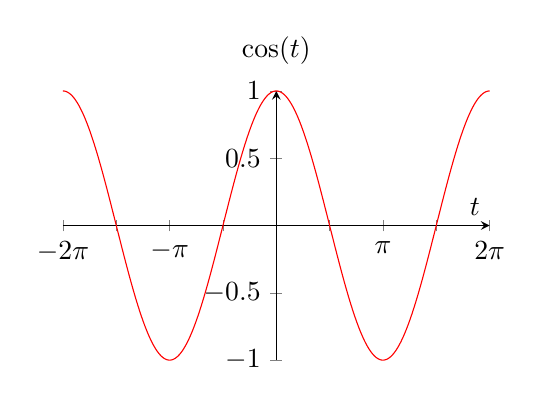
\begin{tikzpicture}
      \begin{axis}[
        title={$\cos(t)$},
        xlabel={$t$},
        axis lines = middle,
        xmax=2*pi,
        xmin=-2*pi,
        height=5cm,
        width=7cm,
        ymin=-1,
        ymax=1,
        xticklabels={$-2\pi$, , $-\pi$, ,
            , $\pi$, , $2\pi$},
        xtick={-6.28318, -4.7123889, -3.14159, -1.5708, 1.5708, 3.14159, 4.7123889, 6.28318}
      ]
        \addplot[red, domain=-2*pi:2*pi, samples=1000]{ cos(deg(x)) };
      \end{axis}
    \end{tikzpicture}
    \caption{Gráfico de $\cos(t)$ en el dominio de tiempo.}
    \label{fig:cos_time_graph}

    \begin{tikzpicture}
      \begin{axis}[
        title={$F(\cos(t))$},
        xlabel={$x$},
        axis lines=middle,
        height=5cm,
        width=6cm,
        xmax=2,
        xmin=-2,
        ymin=0,
        ymax=2
      ]
         \addplot[ycomb, blue, mark=, thick, mark=*] coordinates {
          (1, 1) (-1, 1)
         };
      \end{axis}
    \end{tikzpicture}
    \caption{Gráfico de $F(\cos(t))$ en el dominio de frecuencia.}
    \label{fig:cos_freq_graph}
  \end{multicols}
\end{figure}

La transformada de Fourier es sumamente útil en el procesamiento de señales. La señal que se muestra en la Figura~\ref{fig:cos_time_graph} es una señal continua por lo que se asume que se extiende hasta el infinito. Sin embargo, las computadoras solo puede trabajar con señales finitas y discretas. Esto implica que se tenga que discretizar las funciones continuas como se ve en la Figura~\ref{fig:cos_discrete_time_graph}. Podemos transformar la señal discreta usando la \emph{transformada de Fourier discreta}.
\begin{figure}[ht]
  \centering
  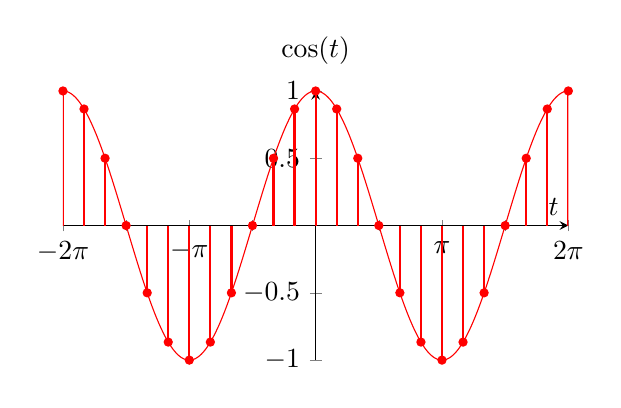
\begin{tikzpicture}
    \begin{axis}[
      title={$\cos(t)$},
      xlabel={$t$},
      axis lines = middle,
      xmax=2*pi,
      xmin=-2*pi,
      height=5cm,
      width=8cm,
      ymin=-1,
      ymax=1,
      xticklabels={$-2\pi$, , $-\pi$, , , $\pi$, , $2\pi$},
      xtick={-6.28318, -4.7123889, -3.14159, -1.5708, 1.5708, 3.14159, 4.7123889, 6.28318}
    ]
      \addplot[ycomb, red, domain=-2*pi:2*pi, samples=25, mark=*, thick, mark size=1.25pt]{ cos(deg(x)) };
      \addplot[red, domain=-2*pi:2*pi, samples=1000, draw]{ cos(deg(x)) };
    \end{axis}
  \end{tikzpicture}
  \caption{Versión discretizada de la función continua $\cos(t)$. Cada punto representa una muestra de la señal. El tiempo entre muestras se denomina tiempo de muestreo.}
  \label{fig:cos_discrete_time_graph}
\end{figure}

La transformada de Fourier discreta se puede ver como una operación lineal. Esto es porque transforma de un vector $N$-dimensional a otro vector $N$-dimensional a través de una matriz de $N \times N$: $F_N$. Para un estado de $n$ qubits, $N$ es igual a $2^n$. Esta transformación se puede escribir como
\begin{equation}
  \ket{x} = \sum_{j=0}^{N-1}x_j\ket{j} \longrightarrow \sum_{k=0}^{N-1}y_k\ket{k},
\end{equation}
donde las amplitudes $y_k$ son las transformadas de Fourier discretas de las amplitudes $x_j$. 
En otras palabras, la transformada de Fourier cuántica (\emph{Quantum Fourier Transform (QFT)}) transforma a los estados de la base estándar de la siguiente manera
\begin{equation} \label{eq:qft}
  F_N\ket{j} = \dfrac{1}{\sqrt N}\sum_{k=0}^{N-1}e^{2\pi i jk/N}\ket{k}.
\end{equation}
Nota que es equivalente a una transformada de Fourier discreta clásica \emph{inversa}. 
La QFT proporciona una aceleración exponencial respecto del algoritmo clásico \emph{FFT:Fast Fourier Transform}.

Ya hemos visto la QFT de un qubit, se trata simplemente de la compuerta Hadamard:
\begin{equation}
  F_2 = H = \hgate.
\end{equation}
Para describir la QFT de $n$-qubits necesitamos las compuertas Hadamard y control fase.
Escribiremos a la compuerta fase como $R_k$ donde
\begin{equation}
  R_k = \begin{pmatrix}
    1 & 0 \\
    0 & e^{2\pi i/2^k}
  \end{pmatrix}.
\end{equation}
En la Figura~\ref{fig: quantum_3_qubit_fourier_circ} se puede observar el circuito para una QFT de 3 qubits. Tener en cuenta que $ S = R_2 $ y $ T = R_3 $. La compuerta cruzada al final es una compuerta de swap, que intercambia dos qubits. El orden de los qubits debe invertirse al final de una QFT para obtener el orden correcto como resultado. De todas formas, invirtiendo el orden de las compuertas y tomando la inversa $ U ^ \ dagger $ de cada compuerta $ U $ da un circuito igualmente eficiente para la transformada cuántica de Fourier inversa $ F_N ^ \ dagger $.

\begin{figure}[ht]
\begin{center}
\begin{quantikz}
\lstick{$\ket{x_0}$} & \gate{H} & \gate{S} & \gate{T} & \qw & \qw & \qw & \swap{2} & \qw \\
\lstick{$\ket{x_1}$} & \qw & \ctrl{-1} & \qw & \gate{H} & \gate{S} & \qw & \qw & \qw \\
\lstick{$\ket{x_2}$} & \qw & \qw & \ctrl{-2} & \qw & \ctrl{-1} & \gate{H} & \targX{} & \qw \\
\end{quantikz}
\end{center}
  \caption{Circuito que realiza la transformada de Fourier cuántica de 3 qubits.}
  \label{fig:quantum_3_qubit_fourier_circ}
\end{figure}
\noindent
Se puede escribir la matriz que implementa la QFT, tomando $\omega = e^{2\pi i/N}$. Para 3 qubits, donde $N = 8$:
\begin{equation}
  F_8 = \dfrac{1}{\sqrt 8}
  \begin{pmatrix}
    1 & 1 & 1 & 1 & 1 & 1 & 1 & 1 \\
    1 & \omega^1 & \omega^2 & \omega^3 & \omega^4 & \omega^5 & \omega^6 & \omega^7 \\
    1 & \omega^2 & \omega^4 & \omega^6 & 1 & \omega^2 & \omega^4 & \omega^6 \\
    1 & \omega^3 & \omega^6 & \omega^1 & \omega^4 & \omega^7 & \omega^2 & \omega^5 \\
    1 & \omega^4 & 1 & \omega^4 & 1 & \omega^4 & 1 & \omega^4 \\
    1 & \omega^5 & \omega^2 & \omega^7 & \omega^4 & \omega^1 & \omega^6 & \omega^3 \\
    1 & \omega^6 & \omega^4 & \omega^2 & 1 & \omega^6 & \omega^4 & \omega^2 \\
    1 & \omega^7 & \omega^6 & \omega^5 & \omega^4 & \omega^3 & \omega^2 & \omega^1 \\
  \end{pmatrix}.
\end{equation}
Un circuito más general para una QFT sobre un estado de $n$ qubits se describe en la Figura~\ref{fig:quantum_fourier_circ}.

\begin{figure}[ht]
\begin{Code}
\begin{center}
\begin{quantikz}[row sep=0.3cm,column sep=0.15cm]%
\lstick{$\ket{x_0}$} & \gate{H} & \gate{R_2} & \qw & \dots & & \gate{R_{n-1}} & \gate{R_n} & \qw & \qw & \qw & \qw & \qw & \qw & \qw & \qw & \qw & \qw & \qw & \qw & \qw \\
\lstick{$\ket{x_1}$} & \qw & \ctrl{-1} & \qw & \dots & & \qw & \qw & \gate{H} & \qw & \dots & & \gate{R_{n-2}} & \gate{R_{n-1}} & \qw & \dots & & \qw & \qw & \qw & \qw \\
\rstick{\vdots} & & & & \vdots & & & & & & & & & & & \\
\lstick{$\ket{x_{n - 1}}$} & \qw & \qw & \qw & \qw & \qw & \ctrl{-3} & \qw & \qw & \qw & \qw & \qw & \ctrl{-2} & \qw & \qw & \dots & & \gate{H} & \gate{R_2} & \qw & \qw \\
\lstick{$\ket{x_n}$} & \qw  & \qw & \qw & \qw & \qw & \qw & \ctrl{-4} & \qw & \qw & \qw & \qw & \qw & \ctrl{-3} & \qw & \dots & & \qw & \ctrl{-1} & \gate{H} & \qw \\
\end{quantikz}
\end{center}
\end{Code}
  \caption{Transformada de Fourier Cuántica sobre $n$ qubits.}
  \label{fig:quantum_fourier_circ}
\end{figure}

El resultado de la transformada de Fourier del estado original se almacena en la amplitudes. 
Sin embargo, recordar que estas amplitudes no se pueden extraer. Por tanto, no hay forma de determinar la transformada de Fourier del estado original usando QFT\@. Aunque no podemos extraer los valores transformados después de una QFT, la QFT tiene su uso en algoritmos cuánticos como el algoritmo de Shor para factorizar enteros y el algoritmo de estimación de fase cuántica.
\newpage

\section{Algoritmo Cuántico de Estimación de Fase}
El algoritmo cuántico de estimación de fase (\emph{QPE} por sus siglas en inglés: Quantum Phase Estimation), estima la fase de un autovector de un operador unitario. Si se prepara un autoestado  $\ket{u}$ de un operador unitario $U$, donde $U\!\ket{u} = e^{2\pi i \varphi}\ket{u}$ 
y el valor de $\varphi$ es desconocido ($0 \le \varphi \le 1$). 
El objetivo es determinar el valor de $\varphi$ 
donde no se conoce necesariamente ni $U$ ni $\ket{u}$, 
pero se tienen cajas negras capaces de preparar $\ket{u}$ 
y aplicar operaciones control-$U$.


\begin{figure}[ht]
\begin{Code}
\begin{center}
\begin{quantikz}[row sep=0.3cm,column sep=0.65cm]%
\lstick{$\ket{0}$} & \gate{H} & \qw & \qw & \qw & \dots & & \ctrl{4} & \gate[4, nwires={2}]{\,F^\dagger_n\,} & \qw & \meter{} & \cw \\
\rstick{\vdots} & & & \vdots & & & & & & & \vdots \\
\lstick{$\ket{0}$} & \gate{H} & \qw & \ctrl{2} & \qw & \dots & & \qw & & \qw & \meter{} & \cw \\
\lstick{$\ket{0}$} & \gate{H} & \ctrl{1} &  \qw & \qw & \dots & & \qw & & \qw & \meter{} & \cw \\
\lstick{$\ket{u}$} & \qw\qwbundle{m} & \gate{U^{2^0}} & \gate{U^{2^1}} & \qw & \dots & & \gate{U^{2^{n-1}}} & \qw & \qw & \qw & \qw \\
\end{quantikz}
\end{center}
\end{Code}
\caption{Circuito del algoritmo de estimación de fase, donde $F^\dagger_n$ 
representa la inversa de la transformada de Fourier de $n$ qubits. La ``/" denota $m$ qubits.}
  \label{fig:phase_estimation_circ}
\end{figure}

El circuito del algoritmo QPE que se observa en la Figura~\ref{fig:phase_estimation_circ} consiste de dos registros. Los $n$ qubits superiores comprenden el primer registro que se utilizará para calcular la estimación de $\varphi$. El tamaño del primer registro se puede elegir en función de dos factores: precisión y probabilidad de éxito. Más qubits darán una mayor precisión y una mayor probabilidad de éxito. Los $m$ qubits inferiores son el segundo registro con los que se preparara el autoestado $\ket{u} $ cuya fase se quiere

Se inicializa el sistema en el estado $\ket{0}^{\otimes n}\ket{u}$. Luego de aplicar $n$ operaciones Hadamard $H^{\otimes n}$ en el primer registro, se tiene el estado
\begin{equation}
  \dfrac{1}{\sqrt{2^n}}(\ket{0} + \ket{1})^{\otimes n} \ket{u}.
\end{equation}
Luego se aplican operaciones control-$U$. Recordando que $U\ket{u} = e^{2\pi i \varphi}\ket{u}$, luego
$U^{2^j}\ket{u} = e^{2\pi i 2^j \varphi}\ket{u}$. Una operación control-$U^{2^j}$ transforma a un estado de la siguiente manera
\begin{figure}[ht]
%\begin{Code}
\begin{center}
\begin{quantikz}%[row sep=0.3cm,column sep=0.65cm]%
\lstick{$\ket{k}$} & \gate{H} & \ctrl{1} & \rstick{$\frac{1}{\sqrt{2}}\left(\ket{0} + e^{2\pi i2^j\varphi}\ket{1}\right)$}\qw \\
\lstick{$\ket{u}$} & \qw\qwbundle{} & \gate{U^{2^j}} & \qw & $\ket{u}$ \\
\end{quantikz}
\end{center}
%\end{Code}
  \caption{Operación Control-$U^{2^j}$ sobre un qubit $\ket{k}$ y autoestado $\ket{u}$.}
  \label{fig:phase_kickback_circ}
\end{figure}
\noindent

Notar que la fase queda en $\ket{k}$ mientras que $\ket{u}$ permanece igual.
Este fenómeno se puede explicar examinando el estado a través de la transformación. El sistema en la  Figura~\ref{fig:phase_kickback_circ} luego de la compuerta Hadamard
se encuentra en el estado
\begin{equation}
  \dfrac{1}{\sqrt2}(\ket{0} + \ket{1})\!\ket{u}
  = \dfrac{1}{\sqrt2}(\ket{0}\!\ket{u} + \ket{1}\!\ket{u}).
\end{equation}
Luego se aplica una control-$U^{2^j}$, es decir,
$U^{2^j}$ solo se aplica cuando el qubit de control ($\ket{k}$) es $\ket{1}$.
Luego se tiene el estado
\begin{align}
  &\dfrac{1}{\sqrt2}\left(\ket{0}\!\ket{u} + \ket{1}U^{2^j}\!\ket{u}\right) \\
  = \, &\dfrac{1}{\sqrt2}\left(\ket{0}\!\ket{u} + \ket{1}e^{2\pi i2^j \varphi}\ket{u}\right) \\
  = \, &\dfrac{1}{\sqrt2}\left(\ket{0} + e^{2\pi i2^j \varphi}\ket{1}\right)\!\ket{u}.
\end{align}

Finalmente, al aplicar los operadores control-$U$ en el circuito QPE como se puede ver en la Figura~\ref{fig:phase_estimation_circ}, el estado del primer registro es
\begin{gather}
  \dfrac{1}{\sqrt{2^n}}\left(\ket{0} + e^{2\pi i 2^{n-1} \varphi}\ket{1}\right)
  \dotsb
  \left(\ket{0} + e^{2\pi i 2^1 \varphi}\ket{1}\right)
  \left(\ket{0} + e^{2\pi i 2^0 \varphi}\ket{1}\right) \\
  = \dfrac{1}{\sqrt{2^n}}\sum_{k=0}^{2^n-1} e^{2\pi i\varphi k}\ket{k}.
\end{gather}
El segundo registro queda en el estado $\ket{u}$. El circuito total luego de las operaciones control-$U$ 
queda en el estado:
\begin{equation} \label{eq:controlled-u-state}
  \dfrac{1}{\sqrt{2^n}}\sum_{k=0}^{2^n-1} e^{2\pi i\varphi k}\ket{k}\!\ket{u}.
\end{equation}
Notar que este estado es similar al resultado obtenido para una  QFT (ver Ecuación \ref{eq:qft}). 
Al aplicar la QFT \emph{inversa} sobre el estado del primer registro
(ver Ecuación \ref{eq:controlled-u-state}) se tiene
\begin{equation}
  \dfrac{1}{2^n}\sum_{k=0}^{2^n-1}\sum_{j=0}^{2^n-1} e^{-2\pi ijk/2^n} e^{2\pi i\varphi k}\ket{j}\!\ket{u}.
\end{equation}

Si $\varphi$ tiene una representación de fracción binaria de $n$ bits $\varphi=j/2^n $, al medir el primer registro en la base computacional nos dará exactamente $\varphi$. Teniendo en cuenta que $\varphi$ no siempre tiene una fracción binaria de $n$ bit. En este caso, obtendremos resultados de medición probabilísticos. La probabilidad $P(j)$ es mayor para valores de grandes de $j$, donde $\varphi\approx j/2^n$, por lo que en este caso solo se puede obtener una aproximación de $\varphi $.

Una idea importante de este algoritmo es la capacidad de la QFT inversa de realizar la transformación
\begin{equation}
  F_{2^n}^\dagger
  \dfrac{1}{\sqrt{2^n}}\sum_{k=0}^{2^n-1} e^{2\pi i\varphi k}\ket{k}\!\ket{u} = \ket{\tilde{\varphi}}\!\ket{u},
\end{equation}
esencialmente permite ``extraer'' una estimación $\ket{\tilde{\varphi}}$ de $\varphi$.

 

% \chapter{Clase 1 - 28 - 08}

\section{Postulados de la mecánica cuántica}

\textbf{1)} \textbf{Sistema aislado}: para cada sistema cuántico uno
le asocia un espacio de Hilbert $\mathcal{H}$de dimensión finita normalizado
con un ket $\KET{\psi}\in\mathcal{H}$

\textbf{2) Medidas:} es un conjunto de operadores $\LLAVES{M_{k},\sum_{k}M_{k}^{\dagger}M_{k}=I}$

Se satisface

$P(k)=\EXPECT{\psi}{\psi}{M_{k}^{\dagger}M_{k}}$, estas dos ecuaciones implican
que $\sum_{k}P(k)=1$

Luego de la medida $\KET{\psi}\rightarrow\frac{M_{k}\KET{\psi}}{\sqrt{P(k)}}$

Medidas proyectivas, caso particular de estas medidas, corresponde
al caso de que los $M_{k}$ son proyectores ortogonales: $M_{k}=P_{k}$,
$P_{k}^{2}=P_{k}$ , $P_{k}P_{l}=\delta_{kl}P_{k}$

\textbf{3)} Para sistema aislado el estado va a \textbf{evolucionar}
de forma unitaria: $\KET{\psi(t_{2})}=U_{t_{2}t_{1}}\KET{\psi(t_{1})}$
en información cuántica no pensamos la evolución temporal como algo continuo
sino más bien como un operador unitario que evoluciona. Si tomamos
como algo continuo llegamos a la ecuación de Schrödinger del operador
unitario.

\textbf{4) Sistemas compuestos }por varios subsistemas: 

\[
\mathcal{H}=\mathcal{H}_{1}\otimes\mathcal{H}_{2}\dots\otimes\mathcal{H}_{n}
\]

\[
\KET{\psi}\in\mathcal{H}
\]

\[
n=2\rightarrow\mathcal{H}=\mathcal{H}_{1}\otimes\mathcal{H}_{2}
\]

Las bases

\[
B_{1}=\LLAVES{\KET{1_{a}}}\quad\text{base de }\mathcal{H}_{1}
\]

\[
B_{2}=\LLAVES{\KET{1_{b}}}\text{base de }\mathcal{H}_{2}
\]

Base de $\mathcal{H}_{1}\otimes\mathcal{H}_{2}=\LLAVES{\KET{1_{a}}\otimes\KET{1_{b}}=\KET{1_{j}}}$

Entonces la $dim\mathscr{\mathcal{H}}=dim\mathscr{\mathcal{H}}_{1}.dim\mathscr{\mathcal{H}}_{2}$

\[
dim\mathscr{\mathcal{H}}=\PARENTESIS{dim\mathscr{\mathcal{H}}_{1}}^{n}
\]

Nos detenemos en este caso, cómo son los estados de este producto
tensorial, queremos puntualizar en el concepto de entrelazamiento.


\section{Entrelazamiento:}

\[
\mathcal{H}=\mathscr{\mathcal{H}}_{1_{A}}\otimes\mathscr{\mathcal{H}}_{2_{B}}
\]

sistemas compuestos: vamos a tomar subsistemas distinguibles. (Los
casos indisttinguibles los podemos hacer tender a sistemas distinguibles
y lo vamos a ver más adelante)

Tenemos estados productos:

\[
\KET{\psi_{AB}}=\KET{\psi_{A}}\otimes\KET{\psi_{B}}\ACLARACION{\text{aligeramos notación}}=\KET{\psi_{A}}\KET{\psi_{B}}
\]

En general: 
\[
\KET{\psi_{AB}}=\sum_{ij}C_{ij}\LLAVEABAJO{\KET{i_{A}}\otimes\KET{j_{B}}}{\KET{ij}}
\]

Si $C_{ij}=\alpha_{i}\beta_{j}$$\KET{\psi_{AB}}=\sum_{i}\PARENTESIS{\alpha_{i}\KET{i_{A}}}\PARENTESIS{\beta_{j}\KET{j_{B}}}=\KET{\psi_{A}}\KET{\psi_{B}}$

$\KET{\psi_{A}}=\sum_{i}\alpha_{i}\KET{i_{A}}$, $\KET{\psi_{B}}=\sum_{j}\beta_{j}\KET{j_{B}}$

\textbf{Estados entrelazados:} (no son estados producto)

\[
\KET{\psi_{AB}}\neq\KET{\psi_{A}}\KET{\psi_{B}}
\]
\emph{Uno no puede hacer combinaciones lineales de los estados que
tiene pero si de los estados producto que tiene.}

Un estado no producto: 
\[
\KET{\psi_{AB}}=\frac{\KET{0_{A}}\KET{0_{B}}+\KET{1_{A}}\KET{1_{B}}}{\sqrt{2}}
\]

esto es una suma de productos pero no es estado producto, esto no
es clásico, ej spines.

Caso más simple, spin 1/2. (Producto)

\[
\KET{\uparrow\uparrow}=\KET{\uparrow}\KET{\uparrow}
\]

ahora bien el estado entrelazado:

\[
\frac{\KET{\uparrow\uparrow}+\KET{\downarrow\downarrow}}{\sqrt{2}}
\]

\[
\BRAKETEO{i_{A}j_{B}}{k_{A}l_{B}}=\BRAKETEO{i_{A}}{k_{A}}\BRAKETEO{j_{B}}{l_{B}}
\]

\[
\KET{\psi_{AB}}=\sum_{ij}C_{ij}\KET{ij}
\]

\[
d_{A/B}=dim(\text{\ensuremath{\mathcal{H}}}_{A/B})
\]

Estado producto: corresponden al caso particular en el que esta matriz
tiene rango 1 $rango(C)=1$ $C:d_{A}\times d_{B}$

\[
C_{ij}=\alpha_{i}\beta_{j}=\left(\begin{array}{c}
\alpha_{i}\\
\vdots\\
\alpha_{d_{A}}
\end{array}\right)\PARENTESIS{\begin{array}{ccc}
\beta_{j} & \dots & \beta_{d_{B}}\end{array}}
\]


\subsubsection{¿Cómo diagonalizar una matriz cuadrada?}

Uno no puede diagonalizar así no más la matriz porque no es cuadrada:

Cualquier matriz se puede escribir como: 
\begin{equation}
\LLAVEABAJO C{d_{A}\times d_{B}}=\LLAVEABAJO U{d_{A}\times d_{A}}\LLAVEABAJO D{d_{A}\times d_{B}}\LLAVEABAJO{V^{\dagger}}{d_{B}\times d_{B}}\label{eq:Cij}
\end{equation}

$D$ diagonal, $U$ y $V$ son unitarias. Tener D diagonal podemos
usarla para escribir mejor $C_{ij}$

\[
D_{kk'}=\delta_{kk'}\sigma_{k}
\]

\[
\sigma_{k}\geq0
\]

\[
C_{ij}=\sum_{k}U_{ik}\sigma_{k}V_{jk}^{*}
\]
a partir de esto todo estado:

\[
\KET{\psi_{AB}}=\sum_{ij}C_{ij}\KET{i_{A}}\KET{i_{B}}
\]

\[
\BRAKETEO{\psi_{AB}}{\psi_{AB}}=1=\sum_{ij}\MODULO{C_{ij}}^{2}=1
\]

Suponemos bases ortogonales

\[
\KET{\psi_{AB}}=\sum_{ijk}\sigma_{k}U_{ik}\KET{i_{A}}V_{jk}^{*}\KET{j_{B}}
\]

\[
=\sum_{k}\sigma_{k}\LLAVEABAJO{\PARENTESIS{\sum_{i}U_{ik}\KET{i_{A}}}}{\KET{k_{A}}}\LLAVEABAJO{\PARENTESIS{\sum_{j}V_{jk}^{*}\KET{j_{B}}}}{\KET{k_{B}}}
\]

\[
=\sum_{k=1}^{n_{s}}\sigma_{k}\KET{k_{A}}\KET{k_{B}}
\]


\subsection{Descomposición de Schmidt}

entonces una descomposición de estados productos uno los puede escribir
con el mismo índice. $n_{s}$ es el número de Schmidt es el rango
de la matriz $C$ (que es igual al de $D$). Los estados productos
son el caso especial donde $n_{s}=1$ $\rightarrow$ \textbf{estado
puro clásico}

Usando la ortogonalidad de los i y de los j llegamos a la ortogonalidad
de los k $\BRAKETEO{k_{A}}{k'_{A}}=\delta_{kk'}$

Pasemos en limpio:

\[
\KET{\psi_{AB}}=\sum_{k=1}^{n_{s}}\sigma_{k}\KET{k_{A}}\KET{k_{B}}
\]

Con $\sum_{k}\sigma_{k}^{2}=1$ acá tenemos 2 casos

$\begin{cases}
\begin{array}{c}
n_{s}=1\rightarrow\KET{\psi_{AB}}=\KET{1_{A}}\KET{1_{B}}\\
n_{s}\geq2
\end{array} & \begin{array}{c}
\text{Estados producto}\\
\text{Estados entrelazados}
\end{array}\end{cases}\begin{array}{c}
\text{sistemas clásicos}\\
\text{sistemas puramente cuánticos}
\end{array}$

\[
n_{s}=rango(C)\leq Min(d_{A},d_{B})
\]

B es el resto del universo, que es muy complejo, pero si el sistema
A vive en un espacio de dimensión 2 entonces el estado más general
posible vive en dimensión 2. Esto indica que si las componentes de
un sistema es de dimensión reducida uno tiene una forma compacta de
escribir el sistema. 

\textbf{¿Cómo calculamos los $\sigma_{k}$?}

De la expresión \ref{eq:Cij} $\underset{d_{B}\times d_{B}}{\underset{d_{B}\times d_{A}}{C^{T}}\underset{d_{A}\times d_{B}}{C}}=VD^{T}U^{T}UDV^{\dagger}=VD^{T}DV^{\dagger}$

\[
\sigma_{k}^{2}=\lambda_{k}\PARENTESIS{C^{T}C}
\]

Análogo con $\underset{d_{A}\times d_{A}}{CC^{T}}=UDD^{T}U^{T}=\lambda_{k}\PARENTESIS{CC^{T}}$ 

\[
\sigma_{k}^{2}=\lambda_{k}\PARENTESIS{CC^{T}}
\]

vamos a obtener solo 2 autovalores, entonces para encontrar los sigmas
los podemos obtener a partir de diagonalizar una matriz de 2x2.

Supongamos el sistema $E$

\[
\mathcal{H}_{A}=\LLAVES{\KET{\uparrow_{A}},\KET{\downarrow_{A}}}
\]

\[
\mathcal{H}_{B}=\LLAVES{\KET{\uparrow_{B}},\KET{\downarrow_{B}}}
\]

Estado singlete, vemos que no es estado producto porque es descomposición
de Schmit

\[
\frac{\KET{\uparrow\downarrow}-\KET{\downarrow\uparrow}}{\sqrt{2}}=\KET{\psi_{AB}}
\]

estado de $S=0$

Estado triplete $S=1$

\[
\frac{\KET{\uparrow\downarrow}+\KET{\downarrow\uparrow}}{\sqrt{2}}
\]

$\frac{\KET{\uparrow\uparrow}\pm\KET{\downarrow\downarrow}}{\sqrt{2}}$
estos tienen $S=\pm1$

Estos son todos ej de estados entrelazados

La $dim\mathcal{H}_{A}=dim\mathcal{H}_{B}=2$ entonces $dim\mathcal{H}_{A}\otimes\mathcal{H}_{B}=4$

Estos estados son una base del sistema.

\subsection{Observable local en A: }

es un operador que corresponden a un observable que son de la forma:
$O_{A}\otimes I_{B}$ (Análogo para B)

$\EXPECT{\psi_{AB}}{\psi_{AB}}{O_{A}\otimes I_{B}}=\sum_{k,k'}\sigma_{k}\sigma_{k'}\LLAVEABAJO{\EXPECT{k_{A}k_{B}}{k_{A}'k'_{B}}{O_{A}\otimes I_{B}}}{\EXPECT{k_{A}}{k'_{A}}{O_{A}}\LLAVEABAJO{\BRAKETEO{k_{B}}{k'_{B}}}{\delta_{kk'}}}$

\[
=\sum_{k}\sigma_{k}^{2}\EXPECT{k_{A}}{k_{A}}{O_{A}}
\]
El estado está en el estado $k_{A}$ con probabilidad $\sigma_{k}^{2}$.

\[
\EXPECT{\psi_{AB}}{\psi_{AB}}{O_{A}\otimes I_{B}}=\text{Tr}\rho_{A}O_{A}
\]
 con $\rho_{A}=\sum_{k}\sigma_{k}^{2}\KET{k_{A}}\BRA{k_{A}}$ este
es el estado reducido del sistema, es un operador densidad.

Uno parte de un estado puro, es un estado de un sistema con T=0, el
estado fundamental del hamiltoniano conjunto. El valor medio del estado
puro viene de la mezcla estadística de estados puros, y esto corresponde
a estados calientes. Es un promedio local de un sistema puro entrelazado.
Un estado total que esta a temperatura 0, cuando uno va al sistema
local lo ve a temperatura distinta de cero, lo puedo ver como un estado
térmico. Uno no puede representar con función de onda el sistema local,
lo tenemos que hacer con un operador densidad (local), estos $\sigma_{k}^{2}$
son los autovalores de los autovectores $\KET{k_{A}}\BRA{k_{A}}$
que surgen de diagonalizar $\rho_{A}$. De forma análoga obtenemos
para $B$:

\[
\EXPECT{\psi_{AB}}{\psi_{AB}}{I_{A}\otimes O_{B}}=\text{Tr}\rho_{B}O_{B}
\]

\[
\rho_{b}=\sum_{k}\sigma_{k}^{2}\KET{k_{B}}\BRA{k_{B}}
\]

Otra de las cosas notables es que el subsistema total esta T=0, los
subsistemas estan calientes, con los mismo autovalores. Los subsistemas
tienen la misma entropía, porque la obtenemos a partir de los $\sigma_{k}$,
$S_{A}=S_{B}$.

\subsection{Operador densidad}

1Cuando uno calcula $\EXPECT{\psi}{\psi}O=Tr\PARENTESIS{\KET{\psi}\BRA{\psi}O}=\sum_{j}\BRAKETEO k{\psi}\EXPECT{\psi}jO$ 

\textbf{Estados puros} corresponden a un \textbf{operador densidad
$\rho=\KET{\psi}\BRA{\psi}$}, proyector ortogonal, satisfaciendo:
$\rho^{2}=\rho$ de rango uno.

En general, un operador densidad general no es un estado puro, es decir
$\rho^{2}\neq\rho$

$\rho=\sum_{i}p_{i}\KET{\psi_{i}}\BRA{\psi_{i}}$, $\BRAKETEO{\psi_{i}}{\psi_{j}}=\delta_{ij}$$p_{i}\geq0$
(esto último $\iff$) 

$\EXPECT{\psi}{\psi}{\rho}=\sum_{i}p_{i}\MODULO{\BRAKETEO{\psi}{\psi}}^{2}\geq0$

Para describir cosas locales necesito operadores densidad porque los
estados puros <<quedan chicos>>. 

\subsection{Matriz densidad reducida: }

dado un estado puro

\[
\KET{\psi_{AB}}\rightarrow\rho_{AB}=\KET{\psi_{AB}}\BRA{\psi_{AB}}
\]
tal que $\EXPECT{\psi_{AB}}{\psi_{AB}}{O_{AB}}=Tr\PARENTESIS{\rho_{AB}O_{AB}}$
con $\rho_{AB}^{2}=\rho_{AB}$

Vamos a lo local:

\[
\EXPECT{\psi_{AB}}{\psi_{AB}}{O_{A}\otimes I_{A}}=Tr\rho_{A}O_{A}
\]
 $\rho_{A}^{2}<\rho_{A}$el menor entre operadores implica que los
autovalores son menores

\[
\KET{\psi_{AB}}=\sum_{k}\sigma_{k}\KET{k_{A}}\KET{k_{B}}
\]

\[
\rho_{A}=\sum_{k}\sigma_{k}^{2}\KET{k_{A}}\BRA{k_{A}}\ACLARACION{\text{traza parcial}}=Tr_{B}\KET{\psi_{AB}}\BRA{\psi_{AB}}
\]

\[
=\sum\LLAVEABAJO{\BRAKETEO{k_{B}}{\psi_{AB}}}{\sigma_{k}\KET{k_{A}}}\LLAVEABAJO{\BRAKETEO{\psi_{AB}}{k_{A}}}{\sigma_{k}\KET{k_{B}}}
\]

\[
\rho_{A}=Tr_{B}\rho_{AB},\qquad\rho_{B}=Tr_{A}\rho_{AB}
\]

\[
Tr_{AB}\rho_{AB}(O_{A}\otimes I_{B})=Tr_{A}(\rho_{A}O_{A})
\]

\[
Tr_{AB}\rho_{AB}(I_{A}\otimes O_{B})=Tr_{B}(\rho_{B}O_{B})
\]

Esto lo tuvimos que introducir (estas trazas parciales ) debido a
que tenemos estados entrelazados.

$\rho_{AB}=\KET{\psi_{AB}}\BRA{\psi_{AB}}$ Puro $\rho_{AB}^{2}=\rho_{AB}$

$\rho_{A}=Tr_{B}\rho_{AB}$ no puro $\rho_{A}^{2}<\rho_{A}$

$\rho_{B}=Tr_{A}\rho_{AB}$ no puro $\rho_{B}^{2}<\rho_{B}$

Si uno tiene una distribución de probabilidades, la queremos caracterizar.
Una cantidad que caracteriza el grado de mezcla es la \textbf{entropía
de Shannon o Von Neumann} $S(\rho_{A})=Tr\rho_{A}\log_{2}\rho_{A}=-\sum_{k}\sigma_{k}^{2}\log_{2}\sigma_{k}^{2}$
(para 0 vale 0: $x\log x\rightarrow0$ cuando $x\rightarrow0$)

Los estados puros $S(\rho)=0\iff\rho^{2}=\rho$ (esta todo concentrado
en un solo evento (1,0,0,0))

Para estados mezcla $S(\rho)>0\iff\rho^{2}<\rho$

Dado un $\rho_{AB}$ puro $S(\rho_{AB})=0$ no hay desorden.

$\rho_{A}=Tr_{B}\rho_{AB}$ no puro entonces $S(\rho_{A})>0$

$\rho_{B}=Tr_{A}\rho_{AB}$ no puro entonces $S(\rho_{B})>0$

luego $S(\rho_{A})=S(\rho_{B})$ 

\subsection{Entropía de entrelazamiento (E)}

\[
S(\rho_{AB}=0)\rightarrow E(A,B)=S(\rho_{A})=S(\rho_{B})
\]

En todo sistema descripto por variables aleatorias (clásico)
\[
S(A,B)\geq S(A)
\]

\[
S(A,B)\geq S(A)
\]

Siendo $S(A,B)$ la entropía de la distribución de probabilidades
conjuntas. $S(AB)=\sum_{ij}p_{ij}\log_{2}p_{ij}$, $S(A)=\sum_{i}p_{i}\log p_{i}$,
$p_{i}=\sum_{j}p_{ij}$

Siempre ocurre esto, sea o no clásico. Vemos que en un estado entrelazado
cambia esto, el desorden global es menor que el desorden local.

La teoría cuántica es una nueva forma de describir sistemas aleatorio,
va más allá de la teoría de probabilidades clásicas. Porque no son
números, son operadores que no conmutan y cambian las cosas en juego.
Entonces esa entropía entrelazada existe, pero no a nivel clásico. 

\paragraph*{El estado entrelazado es una suma de estados productos. Según Schödinger
es LA mecánica cuántica. Es una nueva teoría de descripción de eventos.
Vamos a tener un marco general para describir estos eventos. Luego
vamos a explicar la física de fondo }

% \chapter{Clase 2 - 02 - 09}

\section{Entropía}

\subsection{Entropía de Von Neumann }

\[
S(\rho)=Tr\rho\log_{2}\rho=-\sum_{\nu}\EXPECT{\nu}{\nu}{\rho\log_{2}\rho}
\]


\subsection{Entropía de Shannon}

\[
S(p_{1},\dots,p_{n})=-\sum_{i}p_{i}\log_{2}p_{i}
\]
con $p_{i}\geq0$, $\sum_{i=1}^{n}p_{i}=1$

\[
\rho=\sum_{\nu}\KET{\nu}\BRA{\nu}p_{\nu}
\]

$Tr\rho=1$, $\rho^{\dagger}=\rho$, $\rho\geq0$

\[
S(\rho)=-\sum p_{\nu}\log p_{\nu}
\]
 La entropía de Von Neumann es la extensión de la de Shannon.

\subsection{Propiedades de la entropía}

\textbf{1)} $S(\rho)\geq0$

\textbf{2)} Si $S(\rho)=0$ sii $\rho^{2}=\rho$ es estado puro y
en este caso $p_{1}=1$ y el resto es 0. Ver la dem en la práctica
1. 

\textbf{3) }$S(\rho)$ es máxima sii $p_{1}=\dots=p_{n}=\frac{1}{n}$ 

La entropía es una medida de la falta de información o del grado de
mezcla.

Dado un $\rho_{AB}$ puro $S(\rho_{AB})=0$ no hay desorden.

Repasemos lo de la clase pasada:

Dado un estado conjunto, la descomposición de Schmidt

\[
\KET{\psi_{AB}}=\sum_{ij}^{d_{A},d_{B}}C_{ij}\overset{\KET{i_{A}}\otimes\KET{j_{B}}}{\KET{ij}}=\sum_{k}^{n_{S}}\sigma_{k}\KET{k_{A}k_{B}}
\]

$\sigma_{k}>0$, $\sum_{k=1}^{n_{S}}\sigma_{k}^{2}$, $n_{s}=rango(C)$

$Tr_{B}\LLAVEABAJO{\ketbra{\psi_{AB}}{\psi_{AB}}}{\rho_{AB}}=\rho_{A}=\sum_{k=1}^{n_{s}}\sigma_{k}^{2}\ketbra{k_{A}}{k_{A}}$

$Tr_{A}\LLAVEABAJO{\ketbra{\psi_{AB}}{\psi_{AB}}}{\rho_{AB}}=\rho_{B}=\sum_{k=1}^{n_{s}}\sigma_{k}^{2}\ketbra{k_{B}}{k_{B}}$

$Tr\rho_{AB}O_{AB}=\EXPECT{\psi_{AB}}{\psi_{AB}}{O_{AB}}$

Cuando el operador es un operador local

$Tr\rho_{AB}\PARENTESIS{O_{A}\otimes I_{B}}=\EXPECT{\psi_{AB}}{\psi_{AB}}{O_{A}\otimes I_{B}}=Tr\PARENTESIS{\rho_{A}O_{A}}$

Recordemos entonces que la entropía de entrelazamiento esta definida
como

\[
E(A,B)=S(\rho_{A})=S(\rho_{B})=-\sum_{k}\sigma_{k}^{2}\log_{2}\sigma_{k}^{2}
\]
 Esta entropía solamente proviene de la correlación ya que estos estados
están entrelazados.

$E(A,B)=0\iff n_{s}=1\rightarrow\text{no entrelazado (estado producto)}$

En sistemas cuánticos la entropía no es extensiva, por lo que la entropía
termodinámica (clásica o de variables aleatorias) no nos sirve. Uno
obtiene lo clásico en un límite un particular de lo cuántico.

\section{Qubits}

El sistema más simple posible, donde la $dim\mathcal{H}=2$, la base
de $\mathcal{H}$ es $\LLAVES{\KET 0,\KET 1}$

\[
\KET{\psi}=\alpha\KET 0+\beta\KET 1
\]

con $\MODULO{\alpha}^{2}+\MODULO{\beta}^{2}=1$, la forma más general
de escribir esto es:

\[
\KET{\psi}=\cos\frac{\theta}{2}\KET 0+e^{i\varphi}\sin\frac{\theta}{2}\KET 1
\]

$\rho=\ketbra{\psi}{\psi}$, un estado es un punto en la esfera de
Bloch (esfera de radio 1)

Dada $\sigma_{z}=\PARENTESIS{\begin{array}{cc}
1 & 0\\
0 & -1
\end{array}}$, $\sigma_{z}\KET 0=1\KET 0$, $\sigma_{z}\KET 1=-1\KET 1$

$\sigma_{x}=\PARENTESIS{\begin{array}{cc}
0 & 1\\
1 & 0
\end{array}},\sigma_{y}=\PARENTESIS{\begin{array}{cc}
0 & 1\\
-1 & 0
\end{array}}$, $\sigma_{0}=\PARENTESIS{\begin{array}{cc}
1 & 0\\
0 & 1
\end{array}}$

$S_{z}=\frac{\hbar}{2}\sigma_{z}$, $\vec{S}=\frac{\hbar}{2}\PARENTESIS{\sigma_{x},\sigma_{y},\sigma_{z}}$

$\EXPECT{\psi}{\psi}I=1$, $\EXPECT{\psi}{\psi}{\sigma_{z}}=\cos\theta$,
$\EXPECT{\psi}{\psi}{\sigma_{x}}=\sin\theta\cos\varphi$, $\EXPECT{\psi}{\psi}{\sigma_{y}}=\sin\theta\sin\varphi$
\begin{center}
\includegraphics{pegado32}
\par\end{center}

\subsection{Estado general de un qubit}

Estado puro $\KET{\psi}=\cos\frac{\theta}{2}\KET 0+e^{i\varphi}\sin\frac{\theta}{2}\KET 1$

Estado no puro: $\rho=p\ketbra{\psi_{1}}{\psi_{1}}+(1-p)\ketbra{\psi_{2}}{\psi_{2}}$

En el caso que $\BRAKETEO{\psi_{1}}{\psi_{1}}=0\rightarrow$ $\KET{\psi_{1}},\KET{\psi_{2}}$son
autovectores, $(p,1-p)$ son autovalores de $\rho$. Si no son ortogonales
es un estado mezcla.

$\rho=\alpha\sigma_{0}+\frac{1}{2}\PARENTESIS{r_{x}\sigma_{x}+r_{y}\sigma_{y}+r_{z}\sigma_{z}}$

$Tr(\rho)=1=\alpha TrI+0=2\alpha\rightarrow\alpha=1/2$

\[
Tr(\rho\sigma_{\mu})=\frac{1}{2}2r_{\mu}=\VALMEDIO{\sigma_{\mu}}\rightarrow r_{\mu}=\VALMEDIO{\sigma_{\mu}}
\]

\[
\rho=\frac{1}{2}\PARENTESIS{I+\vec{r}\cdot\vec{\sigma}}\rightarrow\vec{r}=\VALMEDIO{\vec{\sigma}},\MODULO{\vec{r}}\leq1
\]
Un estado mixto en vez de ser un punto sobre la esfera es un punto
dentro de la esfera.

Punto en la esfera: estado puro

Punto dentro de la esfera: estado mezcla

Punto en el centro: estado completamente mezclado. $\rho=\frac{1}{2}I,\:\MODULO{\vec{r}}=0$

La flecha del origen al punto es $\vec{r}$.

\[
\MODULO{\vec{r}}=1\iff\rho\text{ es puro}
\]

\[
0\leq\MODULO{\vec{r}}<1\iff\rho\text{ no puro}
\]

Definamos la dirección $z'\parallel\vec{r}$, entonces $\rho=\frac{1}{2}\PARENTESIS{I+\vec{r}\cdot\vec{\sigma}}=\frac{1}{2}\PARENTESIS{I+\MODULO{\vec{r}}\sigma_{z'}}$.
De aquí: los autovalores de $\rho$ son

$\lambda(\rho)=\frac{1}{2}\PARENTESIS{1\pm\MODULO{\vec{r}}}=\lambda_{\pm}$

$\rho=\lambda_{+}\ketbra{0'}{0'}+\lambda_{-}\ketbra{1'}{1'}$

La polarización de un fotón es una dimensión de un qubit.

\subsection{No cloning theorem}

¿Qué sería una fotocopiadora cuántica?

\[
U\PARENTESIS{\KET{\psi}\LLAVEABAJO{\KET 0}{\text{est. en la hoja a copiar}}}=\KET{\psi}\KET{\psi}\qquad\forall\KET{\psi}
\]

No existe ese operador $U$. Supongamos que si existe y pude crear
otro estado

\[
U\PARENTESIS{\KET{\varphi}\KET 0}=\KET{\varphi}\KET{\varphi}
\]

\[
\PARENTESIS{\BRA{\varphi}\BRA 0}\LLAVEABAJO{U^{\dagger}U}I\PARENTESIS{\KET{\psi}\KET 0}=\BRAKETEO{\varphi}{\psi}\BRAKETEO{\varphi}{\psi}=\BRAKETEO{\varphi}{\psi}^{2}
\]

Entonces $\BRAKETEO{\varphi}{\psi}=\BRAKETEO{\varphi}{\psi}^{2}\rightarrow\BRAKETEO{\varphi}{\psi}=0\;o\;\BRAKETEO{\varphi}{\psi}=1$

Vemos que podemos diseñar $U$ solo que copie estados ortogonales,
pero no sabemos cómo es el estado que va a venir.

\subsection{Representación gráfica de un estado de un qubit}

\[
\underset{t=t_{0}}{\KET{\psi}}\rightarrow\overset{U}{\APLbox}\rightarrow U\underset{t=t_{1}}{\KET{\psi}}
\]

$U=U(t_{1},t_{0})$

Ahora para 2 qubits

\[
\left.\begin{array}{c}
\underset{}{\KET{\psi_{A}}}\rightarrow\overset{U_{A}}{\APLbox}\rightarrow U_{A}\underset{}{\KET{\psi_{A}}}\\
\underset{}{\KET{\psi_{B}}}\rightarrow\overset{U_{B}}{\APLbox}\rightarrow U_{A}\underset{}{\KET{\psi_{B}}}
\end{array}\right\} U_{A}\KET{\psi_{A}}U_{B}\psi_{B}
\]

Ahora si parto de un estado producto 
\[
\KET{\psi_{AB}}=\KET{\psi_{A}}\KET{\psi_{B}}
\]
y el operador unitario $U_{AB}=U_{A}\otimes U_{B}$
\[
U_{AB}\KET{\psi_{AB}}=U_{A}\KET{\psi_{A}}U_{B}\psi_{B}
\]

$U_{A}=e^{-i\frac{H_{A}t}{\hbar}},\quad U_{B}=e^{-i\frac{H_{B}t}{\hbar}}$
, con $t=t_{1}-t_{0}$

Este es un sistema sin interacción, el $H=H_{A}+H_{B}$, este tipo
de hamiltoniano no genera entrelazamiento, un estado producto evoluciona
como estado producto.

\textbf{Otro ejemplo, de un estado no producto:}

\[
\KET{\psi_{AB}}=\frac{\KET{00}+\KET{11}}{\sqrt{2}}
\]
Vemos que ya es un estado en la forma de Schmidt. Este es un estado
entrelazado. 

En cambio el estado $\KET{\psi_{AB}}=\frac{\KET{00}+\KET{01}-\KET{10}-\KET{11}}{2}$
a simple vista no parece estado producto pero rescribamoslo (sacando
factor común al $\KET 0$ y al $\KET 1$):

\[
\frac{\KET 0-\KET 1}{\sqrt{2}}\otimes\frac{\KET 0+\KET 1}{\sqrt{2}}
\]
 vemos que en realidad es un estado producto.

\subsection{Bases:}

\subsubsection{Base computacional:}

\[
\LLAVES{\KET{00},\KET{01},\KET{10},\KET{11}}
\]


\subsubsection{Base de Bell: formada por estados entrelazados:}

$\LLAVES{\frac{\KET{00}\pm\KET{11}}{\sqrt{2}},\frac{\KET{01}\pm\KET{10}}{\sqrt{2}}}$
(estos estados ya estan en la forma de Schmidt. 

En información cuántica nos interesa tener en la base de la forma
de compuertas lógicas.

\section{Compuertas lógicas:}

Ver la figura del primer circuito cuántico, que me genera un estado
entrelazado

\subsection{Hadamard}

\[
H=U_{H}=\frac{1}{\sqrt{2}}\PARENTESIS{\begin{array}{cc}
1 & 1\\
1 & -1
\end{array}}=\frac{1}{\sqrt{2}}\PARENTESIS{\sigma_{z}+\sigma_{x}}
\]

\[
U_{H}\KET 0=\frac{\KET 0+\KET 1}{\sqrt{2}}
\]

\[
U_{H}\KET 1=\frac{\KET 0-\KET 1}{\sqrt{2}}
\]

Me hace la mezcla de estados computacionales en estados equiprobables.

\subsection*{Control not}

\[
U_{CNOT}\KET{00}=\KET{00}
\]

\[
U_{CNOT}\KET{01}=\KET{01}
\]

\[
U_{CNOT}\KET{10}=\KET{11}
\]

\[
U_{CNOT}\KET{11}=\KET{10}
\]

Estas compuertas son completas, esto quiere decir que con cualquiera
de ellas puedo generar cualquier operador unitario. Estos operadores
puedo hacer cualquier tranformación unitaria para cualquier cantidad
de qubits. 

Si uno va cambiando con los estados que entra a estos circuitos voy
a ir obteniendo los diferentes estados de Bell.

% \chapter{Clase 3: 04/09}

La mecánica estadística se justifica como consecuencia de un entrelazamiento
de un estado con su entorno.

Dado un estado entrelazado de 2 qubits

\[
\KET{\psi_{AB}}=\frac{\KET{00}+\KET{11}}{\sqrt{2}}\ACLARACION{\text{el de la derecha es un estado mezcla estadística}}{\neq}\frac{\PROYECT{00}{00}+\PROYECT{11}{11}}{2}
\]

Esta fundamentación general de mecánica estadística parte de que cuando
uno tiene este estado simple entrelazado y hacemos 
\[
Tr_{B}\PROYECT{\psi_{AB}}{\psi_{AB}}=Tr_{B}\PARENTESIS{\frac{\PARENTESIS{\KET{00}+\KET{11}}\PARENTESIS{\BRA{00}+\BRA{11}}}{2}}
\]

\[
=\sum_{\mu=0,1}\BRAKETEO{\mu_{0}}{\psi_{AB}}\BRAKETEO{\psi_{AB}}{\mu_{0}}=\frac{1}{2}\PARENTESIS{\PROYECT 00+\PROYECT 11}=\rho_{A}
\]

\[
\EXPECT{\psi_{AB}}{\psi_{AB}}{O_{A}\otimes I_{B}}=Tr\rho_{A}O_{A}
\]

Para ver los estados fundamentales se estudian sistemas de 2 qubits
haces trazas parcial y ya ves que se genera un estado mezcla (estado
térmico).

\section{Aplicaciones: }

\subsection{Teleportación cuántica (1993)}

Transferir un estado cuántico de un sistema local (Ej. remoto) a través
del entrelazamiento. Entonces es una nueva forma de comunicación. 

Parte de un circuito como el de la clase pasada haces evolucionar
el estado producto y sale un entrelazado como $\KET{\psi_{AB}}$ entonces
esos dos qubits que en su momento no interactuaron cuánticamente salen
entrelazados pero uno fue a un lugar y el otro a otro (los dos caminos
de abajo). Esto se puede usar para transmitir un estado? Propongo
un 3er estado $\KET{\varphi_{C}}=\alpha\KET 0+\beta\KET 1$.

El sistema parte de un estado (\textbf{etapa }I)
\[
\KET{\psi_{CAB}}=\PARENTESIS{\alpha\KET 0+\beta\KET 1}\PARENTESIS{\underset{AB}{\KET{00}}+\KET{11}}/\sqrt{2}
\]

Hacer alguna operación en el planeta A (involucra 2 canales cuánticos,
los dos de arriba) y que el estado $\KET{\psi_{C}}$ aparezca en el
planeta B. La idea es aplicar una medida de Bell (transforma estados
de Bell en estados productos). El entrelazamiento no es espacial si
están a largas distancias mientras el estado no interactuó con otra
cosa no se pierde.

\begin{quantikz}[slice all] \lstick[wires=2]{$\text{Planeta A}$} & \lstick{$\ket{\varphi_c}=\alpha\ket{0}+\beta\ket{1}$}& \ctrl{1} & \gate{H} & & \ctrl{2}&\qw\\ \qw&\qw&\octrl{-1}&\qw&\ctrl{1}&\qw&\qw\\ \lstick[wires=1]{$\text{Planeta B }\ket{\psi_{AB}}=\frac{\ket{00}+\ket{11}}{\sqrt{2}}$}&\qw&\qw&\qw&\gate{\sigma_x}&\gate{\sigma_x}&\rstick{$\ket{\varphi_c}$} 
\end{quantikz}
\begin{center}
\par\end{center}

\textbf{Etapa intermedia II }

Entre el Control-NOT y el Hadamard

\[
\frac{\alpha}{\sqrt{2}}\KET 0\PARENTESIS{\KET{00}+\KET{11}}+\frac{\beta}{\sqrt{2}}\KET 0\PARENTESIS{\KET{10}+\KET{01}}
\]

\textbf{Etapa III}

Después del Hadamard $H\KET 0=\frac{\KET 0+\KET 1}{\sqrt{2}}$ y $H\KET 1=\frac{\KET 0-\KET 1}{\sqrt{2}}$.
Entonces el estado evoluciona a 

\[
\frac{\alpha}{\sqrt{2}}\frac{\KET 0+\KET 1}{\sqrt{2}}\PARENTESIS{\KET{00}+\KET{11}}+\frac{\beta}{\sqrt{2}}\frac{\KET 0-\KET 1}{\sqrt{2}}\PARENTESIS{\KET{10}+\KET{01}}
\]

(todo esto hecho localmente en A)

Si juntamos todo 

\[
=\frac{1}{2}\CORCHETES{\underset{AC}{\KET{00}}\LLAVEABAJO{\PARENTESIS{\alpha\underset{B}{\KET 0}+\beta\underset{B}{\KET 1}}}{\KET{\varphi}}+\KET{01}\LLAVEABAJO{\PARENTESIS{\alpha\KET 1+\beta\KET 0}}{\sigma_{x}\KET{\varphi}}+\KET{10}\LLAVEABAJO{\PARENTESIS{\alpha\KET 0-\beta\KET 1}}{\sigma_{z}\KET{\varphi}}+\KET{11}\LLAVEABAJO{\PARENTESIS{\alpha\KET 1-\beta\KET 0}}{\sigma_{x}\sigma_{z}\KET{\varphi}}}
\]

Entonces si uno después de esto mide en A $\KET{00}$en B aparece
el $\KET 0$.

Lo que vemos es que como consecuencia el estado c o bien paso al otro
lado tal cual o bien paso al otro lado transformado con algún $\sigma_{\nu}$.
Entonces para hacer que el estado original aparezca en el otro planeta
hay 2 opciones:

- Si están cerca y sólo quiero transferir de un cable al otro es hacer
un control si esta $\KET{00}$ no hago nada o si hay $\KET{01}$ hago
$\sigma_{x}$, así sucesivamente (usando que $\sigma_{\nu}^{2}=I$->
anulo la transformación) y así tendría en B en el estado $\KET{\varphi}$.

Si pongo un Control-X $\sigma_{x}$ y un control z, Si está en 1 le
aplica $\sigma_{x}$ ahora en el otro si esta $\KET 1$ aplica $\sigma_{z}$
ahora bien si está en los dos entonces actual los dos. Entonces con
este esquema en la etapa cuatro obtengo en el último canal $\KET{\varphi_{c}}$.
Puedo decir que el entrelazamiento entre A y B se terminó porque se
usó para transferir el estado $\KET{\varphi_{B}}=\alpha\KET 0+\beta\KET 1$. 

Una forma efectiva es modificar el circuito haciendo una medida $\CheckedBox$,
luego esta $\sigma_{x}^{i}$ siendo $i=0,1$ entonces aplica o no
aplica, esto significa una comunicación clásica (la raya curvadita),
llamo y le digo tenés que aplicar la medida. Hago lo mismo con $\sigma_{z}$.
\begin{center}
\includegraphics[scale=0.7]{\string"fig2 clase4-9\string".png}
\par\end{center}

Se usa cristal birrefringente uno de los fotones queda en la tierra
el otro se manda al satélite se hacen las cosas y se prueba esto.

Esto muestra que el entrelazamiento nos permite una nueva forma de
comunicación.

Si hago traza parcial en el canal B antes de los sigmas, 
\[
\rho_{B}=Tr_{AC}\PROYECT{\psi_{CAB}}{\psi_{CAB}}=\frac{\PROYECT 00+\PROYECT 11}{0}
\]

Luego voy a obtener el estado puro $\KET{\varphi}$.

Si hubiera un estado D entrelazado con C, luego de aplicar todo esto
terminaría teniendo el estado D entrelazado con B.

\subsection{Codificación Superdensa}

¿Qué información puede transmitirse con un qubit? La idea es enviar
un qubit. 

Dada una fuente que emite un par de fotones o qubits entrelazados
\[
\KET{\psi_{AB}}=\frac{\KET{00}+\KET{11}}{\sqrt{2}}
\]

En A hacemos una operación U sobre ese qubit. Luego vuelve y hacemos
una medida conjunta en estos dos cables cuánticos.
\begin{center}
\includegraphics[scale=0.5]{\string"fig3 clase4-9\string".png}
\par\end{center}

Si por ej A aplica la I entonces el estado queda igual. 

Si A aplica $\sigma_{x}$, entonces $\KET{\psi_{AB}}\rightarrow\frac{\KET{10}+\KET{01}}{\sqrt{2}}$

Si A aplica $\sigma_{z}$, entonces $\KET{\psi_{AB}}\rightarrow\frac{\KET{00}-\KET{11}}{\sqrt{2}}$

Si A aplica $\sigma_{y}=\sigma_{x}\sigma_{z}$, $\KET{\psi_{AB}}\rightarrow\frac{\KET{10}-\KET{01}}{\sqrt{2}}$

Luego hago la medida conjunta y veo que llego a 4 estados ortogonales
bien distinguidos, entonces si puedo medir estados Bell, pero si recibo
el qubit que viene de A como esta entrelazado voy a poder ver la operación
que hice y voy a obtener 2 bits de información 1 de la operación que
hice y 1 del estado.

Entonces vemos que el entrelazamiento lo podemos usar para transmitir
información. 

Para medir en base estándar mido la polarización directo o con un
stern y gerlach. Ahora bien si quiero hacer medida en la base de Bell,
lo que hago antes de medirlo en la base computacional le aplico alguna
operación para pasarlo de la base de Bell a la computacional: primero
control not y después la Hadamard 
\begin{center}
\includegraphics[scale=0.5]{\string"fig4 clase4-9\string".png}
\par\end{center}

Nosotros sabemos de álgebra que $(AB)^{-1}=B^{-1}A^{-1}$pero dado
que la inversa del Control-NOT es sí mismo y de la Hadamard
es sí misma también, por eso podemos invertir como indica la figura. 

%%%%%%%%%%%%%%%%%%%%Hasta acá esta en algoritmos%%%%%%%%%%%%%%

\section{Demostración de que el desorden global es mayor o igual que el desorden
local en todo sistema descripto por variables aleatorias. (esto es
clásico)}

Tenemos un sistema (A,B) conjunto, entonces tiene una distribución
de probabilidad conjunta
\[
P_{ij}=P(A=i,B=j)
\]
 
\[
S(A,B)=-\sum_{i,j}P_{ij}\log P_{ij}\qquad\text{Medida del desorden global}
\]

\[
S(A,B)=0\iff P_{ij}=\delta_{i}\delta_{j}
\]

\[
S(A,B)\:max\iff P_{ij}=\frac{1}{\sqrt{n_{a}n_{b}}}
\]

Distribución marginal que es $P_{i}^{A}=\sum_{j}P_{ij}$

Entropía de A: $S(A)=-\sum_{i}P_{i}^{A}\log P_{i}^{A}$

Entropía condicional clásica de B dado A $S(B|A)=\sum_{i}P(A=i)\LLAVEABAJO{\sum_{j}P(B=j|A=i)\log P(B=j|A=i)}{S(B|A=i)}$

$P(B=j|A=i)=\frac{P(B=j,A=i)}{P(A=i)}=\frac{P_{ij}}{P_{i}^{A}}$ la
coma significa intersección. 

\[
S(B|A)=-\sum_{i}P_{i}^{A}\sum_{j}\frac{P_{ij}}{P_{i}^{A}}\log\frac{P_{ij}}{P_{i}^{A}}=-\sum_{ij}P_{ij}\PARENTESIS{\log\PARENTESIS{P_{ij}}-\log\PARENTESIS{P_{i}^{A}}}
\]

\[
=S(A,B)-\PARENTESIS{-\sum_{i}P_{i}^{A}\log P_{i}^{A}}=S(A,B)-S(A)\geq0
\]

Que sea $\geq0$ implica que $S(A,B)\geq S(A)$. Entonces el desorden
global es mayor o igual que el desorden local. $\blacksquare$

Ahora bien en un estado de Bell 
\[
\KET{\psi_{AB}}=\frac{\KET{00}+\KET{11}}{\sqrt{2}}
\]
 
\[
\rho_{AB}=\PROYECT{\psi_{AB}}{\psi_{AB}}\qquad\rho_{A}=\frac{\PROYECT 00+\PROYECT 11}{\sqrt{2}}
\]
Ahora ya no tenemos sumas parciales tenemos trazas parciales.
\[
S(A,B)=S(\text{\ensuremath{\rho_{AB}}})=0
\]

Pero ahora $S(\rho_{A})=1=S(A)$ entonces cuánticamente no se cumple
esto.

La entropía condicional cuántica ya no es positiva. 

Para el caso de operadores densidad diagonales:

\[
\rho_{AB}=\sum_{ij}\PROYECT{ij}{ij}p_{ij}
\]
en una base producto (con $p_{ij}>0$), la entropía conjunta se comporta
como una clásica. Tengo un <<mundo clásico>>.

\section{Computación Cuántica}

Idea fundamental (Feymann):

\textbf{Paralelismo cuántico} en un paso puede hacer 2 operaciones
o si más 
\begin{center}
\includegraphics[scale=0.7]{\string"fig5 clase4-9\string".png}
\par\end{center}

Superponer los dos estados es natural es cambiar la dirección del
estado. 

\subsection{El primer algoritmo (histórico) Deutsch 1986.}

El problema más simple posible donde la mecánica cuántica pueda hacer
algo que lo clásico no, entonces dada una función $f:\LLAVES{0,1}\rightarrow\LLAVES{0,1}$
y la pregunta que me hago: $f(0)=f(1)$ o $f(0)\neq f(1)$ que clásicamente
necesita dos evaluaciones de la función pero cuánticamente lo podemos
hacer en una sola evaluación.

Planteo un sistema de dos qubits pero pongo un bloque grande que implica
una operación no sobre un sólo qubit sino una operación que involucra
ambos qubits. Es decir hacerlo con una sóla entrada

Sabemos que $f(0)=0\:o\:1$ al igual que $f(1)$. $U_{f}\KET{ij}=\KET{i,j\oplus f(i)}$
con $\oplus$ suma en módulo 2. Podemos ver que $U_{f}$ es unitaria. 
\begin{center}
\includegraphics[scale=0.75]{\string"fig6 clase4-9\string".png}
\par\end{center}

Entonces qué pasa 
\[
\KET 0\PARENTESIS{\frac{\KET 0-\KET 1}{\sqrt{2}}}=\frac{\KET{00}-\KET{01}}{\sqrt{2}}\underset{U_{f}}{\rightarrow}\frac{U_{f}\KET{00}-U_{f}\KET{01}}{\sqrt{2}}
\]

\[
=\KET{0,f(0)}-\KET{0,1\oplus f(0)}=\KET 0\PARENTESIS{\KET{f(0)}-\KET{1\oplus f(0)}}=(-1)^{f(0)}\KET 0\frac{\KET 0-\KET 1}{\sqrt{2}}
\]

Si $f(0)$ es 0 queda el estado original

Si $f(0)=1$ queda - el estado original

Ahora bien el resultado que uno obtiene de esta suma

\[
\frac{1}{2}\PARENTESIS{\KET 0(-1)^{f(0)}+\KET 1(-1)^{f(1)}}\PARENTESIS{\KET 0-\KET 1}
\]
entonces uno obtiene el valor de $f$ como una fase. 

\[
\frac{1}{2}(-1)^{f(0)}\PARENTESIS{\KET 0+\KET 1(-1)^{f(1)-f(0)}}\PARENTESIS{\KET 0-\KET 1}
\]
Ahí vimos que se puede hacer en un sólo paso. La fase que tenemos
sobre todo el estado no nos importa, ahora bien si $f(0)=f(1)$ entonces
me devuelve el estado original, ahora si $f(0)\neq f(1)$ me da el
estado ortogonal. Mido en la base de x entonces si me da 1 son iguales
si me da -1 son distintas. Vuelvo a ponerlo en la base computacional
con una Hadamard, y obtengo
\begin{center}
\includegraphics[scale=0.7]{\string"fig7 clase4-9\string".png}
\par\end{center}


 
% This ensures that the subsequent sections are being included as root
% items in the bookmark structure of your PDF reader.
\bookmarksetup{startatroot}
\backmatter

\appendix
%\renewcommand{\thechapter}{\alph{chapter}}
\cleardoublepage
% \include{Sources/Apendices}

%  \begingroup
%    \let\clearpage\relax
%    \glsaddall
%    \printglossary[type=\acronymtype]
%    \newpage
%    \printglossary
%  \endgroup

  \printindex
  \printbibliography
\end{document}
